\documentclass[letterpaper, 12pt]{report}
\usepackage[utf8]{inputenc}
\usepackage[spanish]{babel}
\usepackage{graphicx}
\usepackage[left=4cm, right=2.5cm, top=4cm, bottom=2.5cm]{geometry}
\usepackage{titlesec}
\usepackage{caption}
\usepackage{verbatim}
\usepackage{tocloft}
\usepackage{float}
\usepackage[hidelinks]{hyperref}
\usepackage{apacite}
\usepackage{comment}
\usepackage{amsmath}
\usepackage{setspace}
\usepackage{listings}
\usepackage{fancyhdr}
\usepackage{sectsty}
\usepackage{titlesec}
\usepackage{parskip}
\usepackage{chngcntr}
\usepackage{pdflscape}
\usepackage[none]{hyphenat}
\usepackage{microtype}
\usepackage{longtable}
\usepackage{array}
\usepackage{multirow} 

\counterwithout{figure}{chapter}

\pagestyle{fancy}
\fancyhf{}

\onehalfspacing

\renewcommand{\headrulewidth}{0pt}

\titleformat{\chapter}[block]
  {\normalfont\bfseries\Huge}
  {\MakeUppercase\chaptertitlename\ \thechapter: }
  {0pt}
  {\Huge\MakeUppercase}
\titlespacing*{\chapter}{0pt}{-50pt}{40pt}

\chapterfont{\MakeUppercase}
\renewcommand{\contentsname}{ÍNDICE}
\renewcommand{\listfigurename}{ÍNDICE DE FIGURAS}

\setlength{\parindent}{5ex}

\setlength{\parskip}{\baselineskip}

\begin{document}

\begin{titlepage}
  \centering
  \begin{tabular}{@{}p{2cm}@{\hspace{1cm}}p{12cm}@{}}
    \begin{picture}(0,0)
      \put(0,-70){
\includegraphics[width=2cm,height=3cm]{img/logocolor.png}}
    \end{picture}
    &
    \raggedright
    \normalsize UNIVERSIDAD TECNOLÓGICA METROPOLITANA\\
    \normalsize FACULTAD DE INGENIERÍA\\
    \normalsize DEPARTAMENTO DE INFORMÁTICA Y COMPUTACIÓN\\
    \normalsize ESCUELA DE INFORMÁTICA
  \end{tabular}

  \vspace{2.5cm}
  \LARGE \begin{doublespace} MODELO DE APRENDIZAJE AUTOMÁTICO PARA LA PREDICCIÓN DEL COMPORTAMIENTO DE CLIENTES EN CANAL WEB \end{doublespace}
  \vspace{0.1cm}
  \large \begin{singlespace}
    TRABAJO DE TÍTULACIÓN PARA OPTAR AL TÍTULO DE INGENIERO CIVIL EN COMPUTACIÓN MENCIÓN INFORMÁTICA
  \end{singlespace}

  \raggedleft
  \vspace{0.5cm}
  \textbf{\small AUTORES:} \\
  \vspace{0.1cm}
  \small GONZÁLEZ GÁRATE, CRISTÓBAL ANDRES \\
  \vspace{0.1cm}
  \small TAPIA RIQUELME, MARCELO IGNACIO \\
  \vspace{0.1cm}
  \small OYARCE TREJO, DIEGO ESTEBAN \\
  \vspace{0.4cm}
  \textbf{\small PROFESORA GUÍA:} \\
  \small CASTRO OPAZO, PAULA

  \vspace{0.1cm}
  \centering
  \small SANTIAGO - CHILE \\
  \small 2023
\end{titlepage}

\pagenumbering{gobble}

\fancyhf{}

\pagenumbering{roman}
\setcounter{page}{2}
\fancyfoot[R]{\thepage}

\chapter*{Dedicatorias}
\addcontentsline{toc}{chapter}{Dedicatorias}
Este trabajo se lo dedico principalmente a mi madre, Fabiola Trejo, quien ha sido un ejemplo de esfuerzo y lealtad. Sin ella, nada de lo que he logrado hasta ahora podría haber sido posible. Gracias a sus innumerables sacrificios, me fue posible terminar esta larga etapa de mi vida y tener la oportunidad de avanzar con mayor seguridad. Su fortaleza y compromiso me llevaron a donde estoy ahora, finalizando uno de los procesos más importantes que he vivido y que viviré. Estaré eternamente agradecido por su amor, apoyo y confianza.

También quiero dar las gracias a mi hermano, Daniel Oyarce, y a todas mis amistades que me han acompañado durante el proceso de terminar esta carrera. Su compañía fue uno de los pilares que me sostuvo todo este tiempo; su apoyo fue fundamental para mi progreso y sin ellxs no podría haber llegado a donde estoy.

\textit{Diego Oyarce Trejo}

\newpage
Al reflexionar sobre el viaje que ha sido mi carrera universitaria, me siento profundamente agradecido por las numerosas personas que han iluminado mi camino, especialmente en mi inmersión en el fascinante mundo de la informática.

En primer lugar, quiero expresar mi más sincera gratitud a la Profesora Paula Castro Opazo. Su guía experta y la generosidad al compartir su conocimiento han sido fundamentales en el desarrollo y éxito de este proyecto. Su mentoría no sólo ha enriquecido mi experiencia académica, sino que también ha sembrado semillas de sabiduría que florecerán en mi futura carrera.

A mis amados padres, Pamela y Marcelo, les debo mi más profundo agradecimiento. Su amor incondicional, apoyo constante y sabias orientaciones han sido el faro que ha guiado mi viaje. Han sido mi fuente de fortaleza y motivación, permitiéndome encontrar y seguir mi verdadero camino.

A mi amada hermana Constanza, le agradezco por estar siempre presente, escuchando mis preocupaciones y ofreciendo consejos valiosos. Su apoyo ha sido un regalo inestimable en mi vida.

Quiero extender un especial agradecimiento a mis abuelos, Blanca y Rafael, cuya presencia durante mi infancia ha sido un regalo invaluable. Su amor inagotable, sus consejos sabios y su guía constante han sido faros de luz en mi formación. Su influencia ha dejado una huella indeleble en mi corazón y en mi vida, moldeando la persona que soy hoy. Por todo el amor que me han brindado y por sus enseñanzas, les estoy eternamente agradecido.

También quiero reconocer a mi amplia familia, cuyas palabras de aliento y apoyo han resonado fuertemente en cada paso que he dado.

A mis amigos, Andrés, Chelito, David, Cata, Luciano, y muchos otros, gracias por ser parte esencial de mi proceso académico y una invaluable fuente de alegría y camaradería. Los momentos que hemos compartido y el apoyo mutuo que nos hemos brindado ocuparán siempre un lugar especial en mi corazón.

Finalmente, este proyecto no solo marca el cierre de un capítulo significativo en mi vida, sino que también simboliza el comienzo de nuevos horizontes. A todas las personas mencionadas, y a muchas otras que han contribuido a mi viaje, les extiendo mi más sincero agradecimiento. Han dejado una huella imborrable en mi vida y siempre estarán en mi corazón.

\textit{Marcelo Tapia Riquelme}

\newpage
Realmente no sé cómo comenzar esto, solo sé que este es el final de una etapa en mi vida, la cual quizás duro un poco más de lo que hubiese querido, pero no por eso no estoy contento con todo lo que logre aprender, personas que conocí, amistades que se forjaron y experiencias obtenidas.

Cada término de un proceso marca el comienzo de uno nuevo y es por eso, que estoy más que agradecido con todas las personas que estuvieron conmigo durante este camino, las personas que están y que estarán en este nuevo comienzo. Podría nombrar a muchas personas con las cuales pude conectar y nutrirme para poder sobrepasar los obstáculos que se iban presentando en mi camino académico, pero cada uno de ellos sabe quienes son y si en su momento no les agradecí como era debido, les digo gracias, muchas gracias por haber compartido conmigo su tiempo, sobre todo sabiendo que lo material no es lo más importante, si no el tiempo por el cual nosotros como personas transitamos y lo que se hace con él. Quiero extender un agradecimiento a la Profesora Paula Castro Opazo, su apoyo y conocimiento fue fundamental para el desarrollo y éxito de este proyecto.

Agradezco y dedico este trabajo a toda mi familia, la que se encuentra con nosotros y a mis abuelos Carlos González y Adriana Silva que en paz descansan, a pesar de todo nunca dejaron de apoyarme y ayudarme a alcanzar mis metas, no puedo no agradecer a mis abuelos Ricardo Gárate y Ana Vásquez, de los cuales aprendí que todo el esfuerzo y trabajo duro vale la pena, y por sobre todo que lo más importante siempre es la educación, es lo único que nosotros como personas podemos dejar a las generaciones venideras. Aun cuando yo les decía a mis padres que estaba cansado que me dijeran cada vez que los visitábamos “Estudie mijito, que es lo único que sus padres le pueden dejar”, reconozco que siempre tuvo la razón, gracias Tata.

\textit{Cristóbal González Gárate}

\newpage

\chapter*{\centering \large \parbox{\linewidth}{Autorización para la Reproducción \\ del Trabajo de Titulación}}
\addcontentsline{toc}{chapter}{\large Autorización para la Reproducción del Trabajo de Titulación}
\begin{enumerate}
    \item Identificación del trabajo de titulación \\
    Nombre de los alumnos
    :   Cristóbal González G., Marcelo Tapia R. y Diego Oyarce T. \\
    Rut
    : 19.640.046-k , 19.701.282-k , 19.054.592-k \\
    Email
    : cristobal.gonzalezg@utem.cl , marcelo.tapiar@utem.cl , doyarce@utem.cl

    \vspace{0.1cm}

    Título de la tesis
    : Modelo de aprendizaje automático para la predicción del comportamiento de clientes en canal web \\
    Escuela
    : Escuela de Informática \\
    Carrera
    : Ingeniería Civil en Computación Mención en Informática \\
    Título al que opta
    : Ingeniero Civil en Computación Mención Informática \\
    \item Autorización de Reproducción \\
    Este trabajo de titulación no puede reproducirse o transmitirse bajo ninguna forma o por ningún medio o procedimiento, sin permiso escrito de los autores, exceptuando la cita bibliográfica, resumen y metadatos que acreditan al trabajo y a sus autores. \\

    \vspace{3cm}

    \begin{tabular}{@{}l l}
        Fecha: 22/12/2023 \hspace{3cm} & Firma:  \\
        & Cristóbal González G.
    \end{tabular}

    \vspace{3cm}

    \begin{tabular}{@{}l l}
        Fecha: 22/12/2023 \hspace{3cm} & Firma:  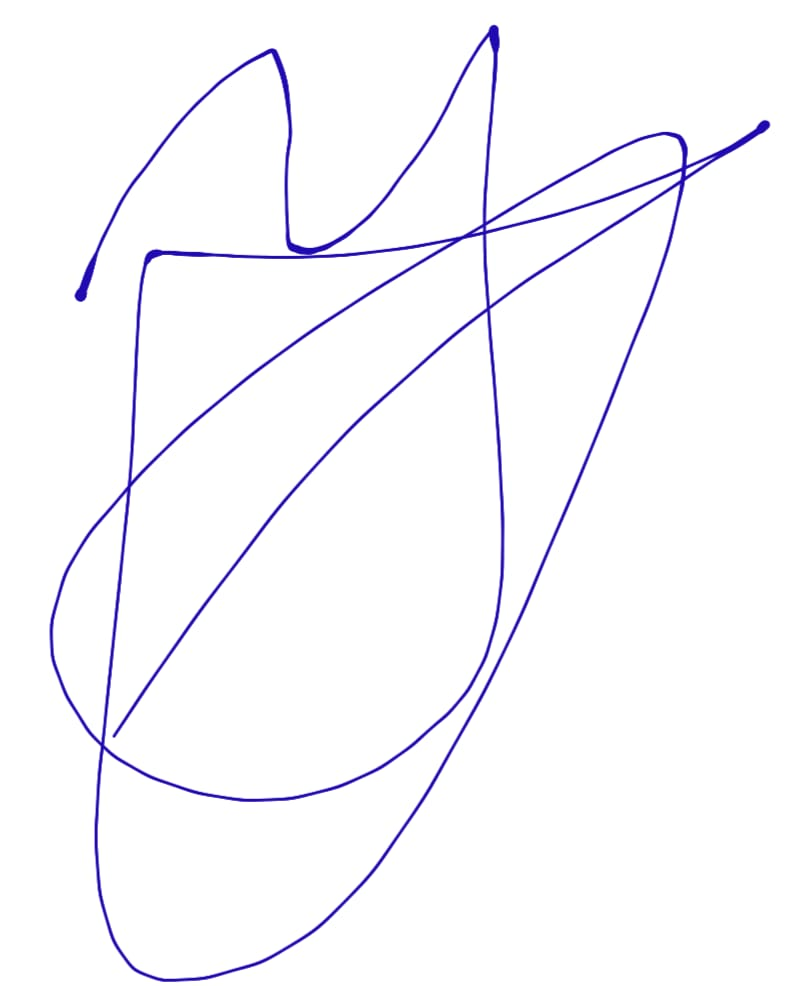
\includegraphics[height=3cm]{img/Firma Marcelo Tapia.jpg} \\
        & Marcelo Tapia R.
    \end{tabular}

    \vspace{1cm}

    \begin{tabular}{@{}l l}
        Fecha: 22/12/2023 \hspace{3cm} & Firma: 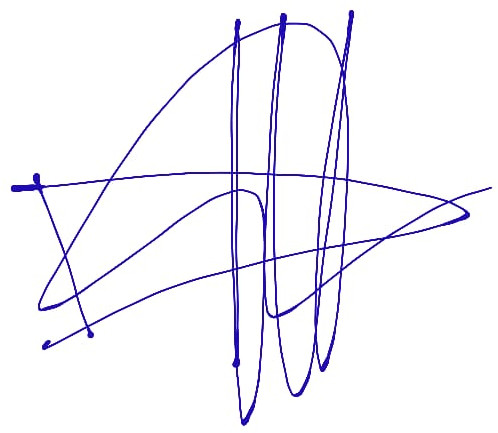
\includegraphics[height=3cm]{img/firma-diego1.jpeg} \\
        & Diego Oyarce T.
    \end{tabular}
\end{enumerate}

Esta autorización se otorga en el marco de la ley N°17.336 sobre Propiedad Intelectual, con carácter gratuito y no exclusivo para la Institución.


\newpage

\tableofcontents

\newpage

\begin{singlespace}
  \listoffigures
\end{singlespace}

\renewcommand{\listtablename}{Índice de tablas}
\begin{singlespace}
  \listoftables
\end{singlespace}

\chapter*{Resumen}
\addcontentsline{toc}{chapter}{Resumen}
El presente documento de Trabajo de Titulación resume exhaustivamente el proceso completo llevado a cabo para desarrollar un modelo de aprendizaje automático capaz de predecir el comportamiento de los usuarios en la nueva plataforma virtual de AFP Capital. Además de detallar la creación de este modelo, se enfoca en la relevancia de la predicción del comportamiento de los clientes y su valor estratégico para las empresas en la actualidad, destacando la importancia de obtener y manejar datos precisos sobre sus comportamientos.

El documento explora varios modelos de aprendizaje considerados como opciones viables, profundizando en la implementación detallada de tres modelos específicos y presentando los resultados obtenidos. Se destaca el proceso de selección del modelo más eficiente entre los evaluados, describiendo minuciosamente este modelo elegido y documentando las pruebas realizadas para demostrar su eficacia final.

Además del desarrollo del modelo, se aborda la creación de un servicio consumible que genera predicciones utilizando el modelo mencionado. Se describe la implementación de una API que facilita la generación de predicciones basadas en los datos de entrada necesarios para el modelo.

El proyecto concluye con la dockerización de todo el trabajo realizado, lo que permite su despliegue simplificado en la plataforma virtual de la empresa. Este enfoque busca garantizar la accesibilidad y la facilidad de implementación del servicio.

Finalmente, se incluyen recomendaciones para mejorar y continuar con el proyecto en caso de que la empresa desee seguir utilizando este modelo. Además, se presentan conclusiones y reflexiones del grupo de trabajo sobre el desarrollo y los hallazgos alcanzados durante el proyecto.

\textbf{Palabras clave:}  Afiliado, Administradora de Fondos de Pensiones, API (Application Programming Interfaces), EDA (Exploratory Data Analysis), Algoritmos de predicción, Algoritmos de clasificación, Modelos de predicción, ETL (Extract, Transform and Load), ARIMA (Modelo de Autorregresión integrada de media móvil), SARIMA (Modelo Estacional de Autorregresión integrada de media móvil), Redes Neuronales Artificiales (ANN), Redes LSTM (Long Short-Term Memory), Redes Neuronales Recurrentes (RNN).

\newpage

\chapter*{Abstract}
\addcontentsline{toc}{chapter}{Abstract}
The purpose of this thesis is to show the form and the work plan used throughout the development process of the proposed project. In addition, the results of the research process that has been carried out to date are presented, including studies on customer behavior in web channels, predictive models and algorithms, and how to develop an ETL process.

The main objective of this project is to analyze AFP Capital's customer behavior and usage preferences over a period of up to 6 months, in order to predict future personalized browsing.

The project consists of four phases for its development. The first phase covers the planning and general background for the realization of the project. The second phase focuses on the investigation of the problem under study, based on the current situation. The third phase covers the modeling and development of the project, including the data modeling and ETL process approach. This phase also involves the development of the code that will support and execute the predictive model, through the construction of databases, APIs and testing to mitigate possible errors found. The fourth and last phase concludes the development of the project and focuses on conclusions and recommendations, where the conclusions obtained throughout the process will be presented, and a ...

\textbf{Keywords:} Affiliate, Pension Fund Administrator, API (Application Programming Interfaces), EDA (Exploratory Data Analysis), Predictive Algorithms, Classification Algorithms, Predictive Models, ETL (Extract, Transform and Load).

\clearpage
\pagenumbering{arabic}
\setcounter{page}{1}
\fancyfoot[R]{\thepage}

\chapter{Presentación del proyecto}
\section{Descripción del trabajo de título}
El trabajo de título se basa en un proyecto que requiere el procesamiento de la data de logs pasados de navegación del sitio web privado de AFP Capital, para detección de comportamientos de clientes y sus preferencias de uso, permitiendo navegaciones futuras customizadas. La lectura de logs será posible gracias a la extracción de dicha información desde Kibana (ElasticSearch), la cual es registrada por APIs variadas que se consumen en el sitio web. Elementos fundamentales del proyecto es el análisis exploratorio de datos, extracciones, transformaciones, cargas, modelo de predicción y detección de preferencias. 

\section{Objetivos}
\subsubsection{Objetivo general}
Analizar el comportamiento de los clientes y sus preferencias de uso en un período igual o inferior a 6 meses, para predecir navegaciones futuras personalizadas. 

\subsubsection{Objetivos específicos }
\begin{itemize}
    \item Realizar una investigación de las herramientas utilizadas para la predicción de comportamiento de usuarios en un canal web.
    \item Llevar a cabo un análisis y estudio de los datos entregados por la empresa. 
    \item Realizar un proceso ETL con la información de navegación web de los clientes de AFP Capital, para analizar su comportamiento dentro del sitio web privado. 
    \item Desarrollar un modelo capaz de predecir el comportamiento de los clientes de AFP Capital, para entregar navegaciones personalizadas futuras.
    \item Establecer recomendaciones de personalización en función de los hallazgos del modelo de predicción para futuras navegaciones dentro del sitio web de AFP Capital.
\end{itemize}

\section{Alcances y Limitaciones}
\subsubsection{Alcances}

El proyecto contempla los siguientes alcances:

\begin{itemize}
\item Se analizará el comportamiento de los clientes de AFP Capital en su nuevo sitio web privado.
\item El proyecto entregará un modelo capaz de predecir el comportamiento de los clientes de AFP Capital en el sitio web, así como una API que permita obtener recomendaciones de comportamiento personalizadas para un afiliado específico.
\end{itemize}

\subsubsection{Limitaciones}

El proyecto tiene las siguientes limitaciones:

\begin{itemize}
\item No se contará con acceso directo a las bases de datos de AFP Capital, por lo tanto, se trabajará con una muestra de datos.
\item No se podrá acceder a información sensible de los clientes de AFP Capital, como los RUTs (Rol Único Tributario) u otra información personal identificable.
\item El análisis se basará únicamente en datos cualitativos de la navegación web de los usuarios.
\end{itemize}

\chapter{La empresa}
AFP Capital se erige como un actor destacado en su industria, con una trayectoria consolidada y un enfoque constante en la innovación y la excelencia operativa. Este capítulo del informe proporcionará una visión detallada de su historia, una descripción general, misión, visión y su papel en el mercado actual. A lo largo de estas páginas, exploraremos los aspectos clave que definen a esta empresa y su relevancia en el panorama empresarial actual.




\section{Historia}
La historia de AFP Capital se remonta a noviembre de 1980, cuando se implementó en Chile el sistema de pensiones de capitalización individual. El 16 de enero de 1981, se constituyó la sociedad Administradora de Fondos de Pensiones Santa María, que más tarde se transformaría en AFP Capital S.A. Desde sus inicios, la empresa se destacó por su filosofía de servicio, enfocada en satisfacer las necesidades y expectativas de sus afiliados. 
En 1995, AFP Capital estableció la filial Santa María Internacional S.A., con el propósito de expandir su alcance y ofrecer servicios a personas naturales o jurídicas del extranjero, así como invertir en AFP o sociedades relacionadas con materias previsionales en otros países. Esta iniciativa consolidó la presencia de AFP Capital en el ámbito internacional y fortaleció su posición como una administradora de fondos de pensiones líder en la región. 
En el año 2000, se produjo una relevante transacción en la historia de AFP Capital. ING Group adquirió Aetna Inc., incluyendo el 96,56\% de las acciones de AFP Capital S.A. Esta adquisición tuvo como objetivo reforzar la posición de liderazgo de AFP Capital en el mercado previsional chileno y contribuir a su crecimiento y desarrollo. 
Posteriormente, en 2008, AFP Capital llevó a cabo una fusión con AFP Bansander, otra reconocida administradora de fondos de pensiones en Chile. Esta fusión permitió consolidar aún más las operaciones de AFP Capital y fortalecer su presencia en el país. A fines de 2011, Grupo SURA, una empresa líder en el negocio de pensiones en Latinoamérica, adquirió las operaciones de ING en la región. Esta adquisición llevó a AFP Capital a formar parte de Grupo SURA y a beneficiarse de su amplia experiencia y recursos, consolidándose como una compañía destacada en el mercado previsional latinoamericano. En resumen, la historia de AFP Capital está marcada por su constante evolución, consolidación y liderazgo en el mercado de administración de fondos de pensiones en Chile. A lo largo de los años, ha demostrado su compromiso con la excelencia en la prestación de servicios previsionales y su capacidad de adaptación a los cambios y desafíos del entorno económico y regulatorio.

\begin{figure}[H]
    \begin{minipage}[t]{0.9\textwidth}
        \caption{Historia AFP Capital}
        \label{historia-afp}        
    \end{minipage}

    \vspace{10pt}

    \begin{minipage}[b]{1.1\textwidth}
        \centering
        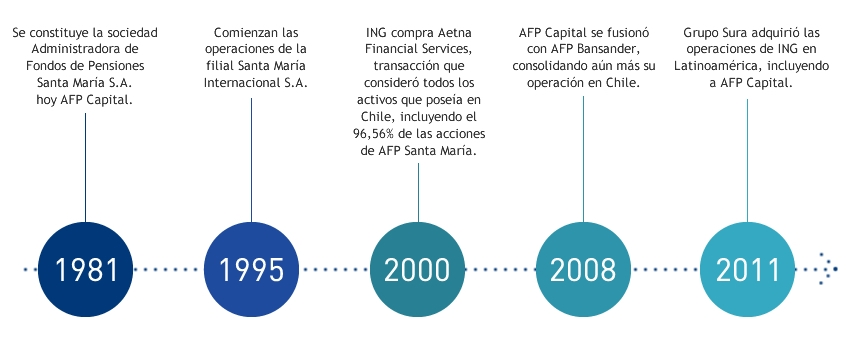
\includegraphics[width=\textwidth]{img/historia-afp-capital.jpg}        
    \end{minipage}

    \begin{minipage}[t]{0.9\textwidth}
        Fuente: AFP Capital. Recuperado de \url{https://www.afpcapital.cl/Quienes-Somos/Paginas/Historia.aspx}
    \end{minipage}
\end{figure}
%agregar la imágen de la historia%

\section{Descripción general}
\input{La empresa/Descripción general}

\section{Misión y visión}
\subsection{Misión}
\input{La empresa/Misión.tex}
\subsection{Visión}
\input{La empresa/Visión.tex}

\chapter{Marco teórico}
En el ámbito empresarial actual, la capacidad de predecir y comprender el comportamiento del cliente en un sitio web es esencial para el éxito. Este capítulo del informe se adentrará en la importancia estratégica de estas predicciones, analizará el comportamiento de los clientes y afiliados en el canal web y presentará las herramientas clave utilizadas para anticipar y optimizar la experiencia del usuario en línea.
\section{Importancia de predecir el comportamiento del cliente en un sitio web}
La predicción del comportamiento del cliente dentro de un entorno web se considera a la aplicación de técnicas y modelos analíticos para lograr predecir en cierta manera las posibles necesidades, acciones, preferencias y decisiones que un cliente pueda tomar mientras interactúa en alguna plataforma en línea o sitio web. En los últimos años, ha sido de gran importancia la predicción del comportamiento de los clientes para las empresas, gracias a esto buscan anticipar las necesidades y preferencias de sus clientes, pudiendo adaptar los productos y servicios para entregar una mayor satisfacción al cliente (Zheng, Thompson, Lam, Yoon y Gnanasambandam, 2013). La lealtad de los clientes representa un valor clave para las empresas, ya que un cliente leal seguirá consumiendo los productos y servicios de la empresa, por lo que si se mejora la experiencia del usuario, la satisfacción del cliente aumenta y esto genera un aumento en la ganancia de la empresa. 
Según Zheng, Thompson, Lam, Yoon y Gnanasambandam (2013), la predicción del comportamiento del cliente ayuda a las empresas a identificar oportunidades de mejora y mercado, además de ayudar a tomar decisiones informadas sobre estrategias de publicidad y marketing. El objetivo fundamental de predecir el comportamiento del cliente en un entorno web es lograr comprender y anticipar las acciones de los clientes con la meta de personalizar, mejorar la experiencia de usuario y poder aumentar la satisfacción y fidelidad de los clientes. 
Las predicciones pueden abarcar distintos aspectos del comportamiento de un cliente dentro de un canal web, a grandes rasgos existen 4 tipos de predicciones que se pueden realizar, están las predicciones de compras, donde mediante el análisis de patrones de navegación, su historial de compras, preferencias y características demográficas, gracias a esto se busca predecir las compras futuras de un cliente, se encuentra la predicción de clics, esta busca anticipar los enlaces o elementos con los cuales un cliente va a interactuar dentro de un sitio web, lo que busca mejorar la calidad de contenido que se encuentra desplegado y lograr mejorar la usabilidad del sitio web, también está presente la predicción de abandono de carrito, esta permite tomar acciones de recuperación o retención del cliente, se concentra en identificar aquellos clientes que agregan productos a un carrito de compra pero no finalizan el proceso de compra y por ultimo, esta la predicción de retención de clientes, esta busca predecir qué clientes están más cercanos a abandonar o terminar la relación existente con el sitio web, para poder generar e implementar estrategias para aumentar la fidelización y retención de estos clientes. 



\section{Comportamiento del cliente/afiliado en el canal web}
\subsection{Definición y relevancia del comportamiento del cliente para el negocio}
Considerando los modelos de negocios establecidos por las Administradoras de Fondos de Pensiones [AFP], de ahí radica la importancia de la figura del cliente. Según lo que indica la Real Academia Española, el cliente es la persona que realiza una compra o utiliza los servicios que un profesional o empresa pueda ofrecer (Real Academia Española, s.f), no obstante en base al sistema establecido por las Administradoras de Fondos de Pensiones, el cliente obtiene el nombre de afiliado pues estos contribuyen o se encuentran inscritos en un plan de pensiones (Rasekhi, Fard y Kim, 2016). 
El afiliado es el centro del negocio, cuya gran importancia radica principalmente en la rentabilidad que brinda. Cada trabajador que decida afiliarse se traduce en una ganancia, mientras que cada afiliado que decida desafiliarse genera perdida. Considerando esto es que se puede apreciar la segunda importancia del afiliado, debido a que este promueve la marca si es que la experiencia del servicio de cara al usuario es buena. En tercer lugar, el afiliado, al ser un ganancia para el modelo, este a su vez que obtiene el servicio es capaz de posibilitar el crecimiento de la empresa al tener su preferencia. Por otro lado, la experiencia del cliente y su feedback es valiosa ya que puede brindar conocimiento de los puntos débiles y con posibilidad de mejora que tiene el sistema (Rodriguez, 2023). 
Dentro de las distintas funciones que el cliente tiene, en primer lugar se puede mencionar al cliente como consumidor. Consiste en unas de las funcionalidades más tradicionales puesto que el objetivo intrínseco del cliente es consumir o contratar servicios. Como consumidor es quien adquiere un producto o servicio y lo aprovecha para un fin o necesidad, por lo que la empresa obtiene su principal fuente de ingresos.
En segundo lugar, se tiene al cliente como prosumidor, en otras palabras, consume y produce a la vez (Toffler, 1980). Al momento del consumo, el cliente también deja reseñas o realiza comentarios en lugares especializados, información que resulta de utilidad para generar insights que mejoren la experiencia en el servicio. 
En tercer lugar, se entiende al cliente como crítico, puesto que si la experiencia del cliente es negativa, el feedback y reseñas negativas que este brinde pueden ser de índole constructiva como destructiva. 
En cuarto lugar, se encuentra el cliente como pieza fundamental en el desarrollo de los productos y servicios. Los comentarios de los clientes pueden conducir al desarrollo de servicios innovadores apegados a las necesidades que los clientes indican. Para poder lograr perfeccionar el servicio y productos ofrecidos, es crucial el aporte de los clientes recurrentes o suscriptores del servicio, en el caso específico de las Administradoras de Fondos de Pensiones se refiere a los afiliados. 
En quinto lugar, el cliente como evaluador de la experiencia. Relacionado con los puntos anteriores, la mejor forma de mejorar la experiencia del cliente es tomando en consideración los comentarios de los clientes en esta materia, así se puede generar una diferencia de las otras empresas que constituyen la competencia existente en el mercado. 
Por último, se considera que el cliente puede ser un eventual embajador de la marca, en otras palabras promotores de la misma pudiendo generar recomendaciones, comentarios y reseñas positivas que promuevan el negocio. 


\subsection{Características del comportamiento del cliente en el canal web}
Para comprender la experiencia y el comportamiento del cliente en un canal web, es importante reconocer la existencia del customer journey, el cual describe las distintas etapas por las que un cliente pasa al consumir un producto o servicio. Según \cite{lemon2016customer}, estas etapas incluyen la conciencia, investigación, consideración, compra, uso y evaluación. La etapa de conciencia refiere a la identificación de una necesidad o problema que debe ser resuelto, mientras que la investigación implica la búsqueda de información por parte del cliente para encontrar posibles soluciones y comparar entre diferentes opciones disponibles. Luego, en la etapa de consideración, el cliente evalúa las alternativas y elige la que mejor se adapte a sus necesidades, lo que lleva a la etapa de compra, donde se realiza la contratación o adquisición del servicio seleccionado. Posteriormente, viene la etapa de uso, en la cual el cliente experimenta y evalúa la calidad, funcionalidad y experiencia del servicio. Por último, se encuentra la etapa de evaluación, en la cual el cliente emite un feedback voluntario, tanto positivo como negativo, sobre su experiencia satisfactoria o insatisfactoria. En resumen, las opciones disponibles en el canal web buscan hacer del customer journey una experiencia eficiente y agradable.

En cuanto al segundo párrafo, parece contener información específica sobre el canal web de AFP Capital y las opciones disponibles para los afiliados. Sin embargo, la estructura y organización del texto pueden mejorarse para una mayor claridad. Aquí está el párrafo revisado:

Para acceder al canal web de AFP Capital, es necesario ser afiliado y contar con una cuenta privada personal que incluya el RUT y contraseña. Una vez ingresado al canal web privado, los afiliados tienen a su disposición diversas opciones para satisfacer sus necesidades. Estas incluyen revisión del pago o no de la cotización mensual, la obtención de certificados de cotizaciones, afiliación, antecedentes previsionales y traspaso de fondos, así como certificados tributarios. Además, se pueden obtener certificados generales, como de residencia, suscripción de ahorro previsional voluntario (APV), cuenta 2, remuneraciones imponibles, periodos no cotizados y trabajo pesado. En el caso de afiliados pensionados, también se pueden obtener certificados de asignación familiar, calidad de pensionado, pensiones pagadas, pensión en trámite, ingreso base y comprobante de pago de pensión. Además, es posible acceder a la cartola en línea. El canal web privado permite realizar el ahorro obligatorio y voluntario, inversiones, depósitos directos, consultar planillas de pagos y ver las comisiones cobradas como afiliado. También ofrece la opción de verificar el fondo de pensiones, los tipos de fondos disponibles (A, B, C, D, E) y sus porcentajes de rentabilidad, así como realizar cambios de fondo de pensiones y acceder a educación previsional. Además, se brinda la posibilidad de realizar giros en cuentas personales, acceder a rescates financieros y tramitar la pensión.

\subsection{Factores que afectan el comportamiento del cliente}
%Factores que influyen en el comportamiento del cliente en el canal web, tales como la usabilidad y el diseño del sitio web.
Lemon y Verhoef (2016) proponen que los principales factores que influyen en el comportamiento del usuario y su experiencia son sensoriales, afectivos, cognitivos, puntos de contacto y externos. Dentro de la experiencia sensorial se encuentra lo apreciable con alguno de los sentidos del cuerpo, tanto vista, olor, tacto, entre otros. Respecto de la experiencia afectiva, hay que tener en consideración la emocionalidad del cliente producto de la experiencia del producto o del servicio. Al hablar del aspecto cognitivo, este refiere de los pensamientos, creencias y/o actitudes que el cliente pueda tener respecto de la compañía, el producto o el servicio entregado. Sobre los puntos de contacto, estos hacen mención a las distintas maneras en las que el cliente y la compañía entran en contacto, tales como la publicidad, servicio al cliente, redes sociales o interacciones de tipo transaccional (Lemon y Verhoef, 2016). Por último, el factor externo cuya definición hace referencia a considerar el contexto actual, las condiciones socioeconómicas y otros factores que puedan afectar la experiencia del usuario que se encuentren fuera de control de la compañía. 
Dentro de los factores que pueden influir en el comportamiento de un cliente en el canal web están principalmente, la usabilidad y el diseño. Respecto a la usabilidad, esta depende de 7 características las que garantizan una buena experiencia del usuario. Según Sanchez (2011) la accesibilidad, legibilidad, navegabilidad, facilidad de aprendizaje, velocidad de utilización, eficiencia del usuario y tasas de error del canal web, influyen en la experiencia y posterior feedback que el usuario pueda brindar sobre el uso de los servicios. 
Por otro lado, el diseño del sitio web depende de 5 características para garantizar un buen contenido y estética para lograr que el usuario encuentre lo que busca en el menor tiempo posible, en otras palabras, eficiencia. El autor Walter Sanchez (2011) indica que el diseño debe de ser entendible, novedoso, comprensible, inteligente y atractivo, consiguiendo acercar los contenidos de mejor manera al usuario y logrando conseguir una navegación más intuitiva. Estos factores son de gran importancia para que el usuario pueda encontrar el contenido que busca en el menor tiempo posible y que la experiencia sea positiva al interactuar con la interfaz del sitio web. 


\section{Herramientas para la predicción del comportamiento del cliente en el canal web}

\subsection{Introducción a las herramientas de análisis de datos}
En el entorno empresarial actual, la capacidad de tomar decisiones informadas y basadas en datos se ha vuelto fundamental para el éxito y la competitividad de las organizaciones. El análisis de datos desempeña un papel crucial en este proceso, permitiendo a las empresas obtener información valiosa a partir de grandes volúmenes de datos y utilizarla para comprender el comportamiento del cliente de manera más profunda y precisa. Esto resulta de suma importancia, ya que la calidad de las decisiones tomadas marca la diferencia entre el éxito y el fracaso \cite{analitica-predictiva}.

Dentro de las herramientas de análisis de datos, se destacan cuatro conceptos clave que han revolucionado la forma en que se procesan y se obtiene información de los datos: Business Intelligence, Big Data, Machine Learning y Data Mining. Estas herramientas proporcionan a las empresas la capacidad de extraer conocimientos y patrones significativos de los datos, lo que a su vez les permite tomar decisiones estratégicas más acertadas y personalizar sus estrategias de marketing y atención al cliente.

El Business Intelligence (BI) se refiere a la recopilación, análisis y presentación de datos empresariales para facilitar la toma de decisiones. Mediante el uso de diversas técnicas y herramientas, el BI permite a las empresas visualizar y comprender mejor los datos de sus operaciones y clientes. Esto incluye la generación de informes, el análisis de tendencias, la monitorización de indicadores clave de rendimiento (KPI) y la creación de tableros de control interactivos. El BI ayuda a las organizaciones a identificar oportunidades, detectar áreas de mejora y optimizar su rendimiento en función de datos históricos y en tiempo real. Sobre la inteligencia de negocios, se ha determinado que cada implementación es única para cada proceso empresarial \cite{analitica-empresarial}.

El Big Data se refiere a la gestión y análisis de grandes volúmenes de datos, tanto estructurados como no estructurados, que superan la capacidad de las herramientas tradicionales de almacenamiento y procesamiento. El Big Data se caracteriza por las tres V's: Volumen (gran cantidad de datos), Velocidad (alta velocidad de generación y procesamiento de datos) y Variedad (diversidad de fuentes y formatos de datos). Para aprovechar el potencial del Big Data, las empresas emplean técnicas de procesamiento distribuido y herramientas específicas para el almacenamiento, procesamiento y análisis de estos datos masivos. El análisis de Big Data permite identificar patrones, tendencias y correlaciones ocultas en los datos, lo que brinda información valiosa para entender y anticipar el comportamiento del cliente.

El Machine Learning (aprendizaje automático) es una rama de la inteligencia artificial que permite a los sistemas informáticos aprender y mejorar automáticamente a partir de la experiencia sin ser programados explícitamente. En lugar de basarse en una analítica descriptiva, el Machine Learning ofrece una analítica predictiva \cite{inteligencia-negocios}. Mediante algoritmos y modelos, el Machine Learning permite a las empresas analizar grandes conjuntos de datos y detectar patrones complejos en el comportamiento del cliente. Esto permite realizar predicciones y recomendaciones personalizadas, así como automatizar tareas y procesos, lo que mejora la eficiencia operativa y la experiencia del cliente.

El Data Mining (minería de datos) se refiere al proceso de descubrir información valiosa, patrones y relaciones desconocidas en grandes conjuntos de datos. Utilizando técnicas estadísticas y algoritmos avanzados, el Data Mining permite identificar correlaciones y tendencias ocultas en los datos, lo que ayuda a las empresas a comprender mejor el comportamiento del cliente y tomar decisiones más acertadas. Esta herramienta es especialmente útil para la segmentación de clientes, la detección de fraudes, la recomendación de productos y la personalización de ofertas.


\subsection{Métodos, técnicas y tecnologías de análisis de datos}
En el análisis de datos para predecir el comportamiento del cliente, se utilizan una variedad de métodos, técnicas y tecnologías que permiten procesar y analizar grandes volúmenes de información con el fin de obtener información valiosa. Estas herramientas proporcionan a las empresas y organizaciones la capacidad de comprender mejor a sus clientes, identificar patrones y tendencias, y tomar decisiones estratégicas más acertadas.

Entre los métodos y modelos más utilizados se encuentran la regresión logística, que permite predecir la probabilidad de que un cliente realice una determinada acción o tome una decisión; el clustering, que agrupa a los clientes en segmentos o categorías similares con características y comportamientos comunes; los árboles de decisión, que representan un conjunto de reglas lógicas para clasificar a los clientes en diferentes grupos; el Random Forest, que combina múltiples árboles de decisión para mejorar la precisión de las predicciones; y el Gradient Boosting Machine, que utiliza múltiples modelos de aprendizaje débiles para construir un modelo más robusto y preciso.

Además de los métodos y modelos, existen diversas técnicas que se aplican en el análisis de datos para predecir el comportamiento del cliente. Entre ellas se encuentran las redes neuronales artificiales (ANN), que son modelos inspirados en el funcionamiento del cerebro humano y se utilizan para reconocer patrones y realizar predicciones complejas; y el Support Vector Machine (SVM), que es un algoritmo de aprendizaje automático utilizado para clasificar y predecir datos.

En cuanto a las tecnologías utilizadas en el análisis de datos, se destacan diversas herramientas y lenguajes de programación. Algunas de las más populares son Tableau, que permite visualizar y explorar los datos de manera interactiva; Python, con bibliotecas como Pandas, NumPy y Scikit-learn, que ofrecen una amplia gama de funciones y algoritmos para el análisis de datos; R, con paquetes como dplyr, caret y randomForest, que brindan herramientas estadísticas y de aprendizaje automático; Apache Spark, que permite procesar y analizar grandes volúmenes de datos de manera distribuida; KNIME y RapidMiner, que son plataformas de análisis de datos visuales; y QlikView y Power BI, que son herramientas de visualización de datos y creación de tableros de control.

\subsection{Modelos de predicción de comportamiento del cliente}
En la era digital, los modelos de predicción de comportamiento del cliente son un recurso fundamental para las empresas que buscan tomar decisiones informadas y personalizar sus estrategias. Este subcapítulo del informe se adentrará en los diversos modelos utilizados para anticipar las acciones y preferencias de los clientes, destacando su relevancia en la toma de decisiones estratégicas y la mejora de la experiencia del usuario en el entorno online.


\subsubsection{Modelos de regresión logística}
\subsubsection{Modelos de regresión}
\noindent
La regresión logística corresponde a un algoritmo de aprendizaje automático supervisado que es empleado para resolver problemas de clasificación. Si bien, su nombre contiene “regresión”, en realidad corresponde a un método de clasificación.

Se da uso a la regresión logística cuando la variable de respuesta o variable objetivo es categórica. En lugar de predecir un valor numérico como en la regresión lineal, la regresión logística estima la probabilidad de que una observación pertenezca a una categoría específica.

Los modelos de regresión logística se basan en la función logística, también conocida como función sigmoide, que mapea cualquier valor real a un rango entre 0 y 1. La función sigmoide tiene la siguiente forma matemática:

\begin{equation*}
    f(z) = \frac{1}{(1 + e^{-z})}
\end{equation*}

En la regresión logística, se ajusta un modelo lineal a los datos de entrada y se aplica la función sigmoide al resultado para obtener la probabilidad de pertenencia a una clase. La ecuación del modelo se expresa como:

\begin{equation*}
    p(y=1|x) = \frac{1}{(1 + e^{(-(b0 + b1x1 + b2x2 + ... + bn*xn))})}
\end{equation*}

Donde:

p(y=1|x) es la probabilidad condicional de que la variable de respuesta sea igual a 1 dada la entrada x.

b0, b1, b2, ..., bn son los coeficientes del modelo que se ajustan durante el proceso de entrenamiento.

x1, x2, ..., xn son los valores de las variables de entrada.

El proceso de ajuste de la regresión logística implica encontrar los mejores valores para los coeficientes del modelo con la finalidad de maximizar la verosimilitud de los datos observados. Esto se puede hacer mediante métodos numéricos como la maximización de la función de verosimilitud o mediante algoritmos de optimización como el gradiente descendente.

Una vez entrenado el modelo, se puede utilizar para hacer predicciones clasificando nuevas observaciones según la probabilidad estimada. Por ejemplo, si la probabilidad estimada de pertenencia a una clase es superior a un umbral (generalmente 0.5), se clasificará como perteneciente a esa clase.

Para nuestro caso en particular, puede ser utilizado el modelo de regresión logística para predecir el comportamiento de usuarios en un canal web, para ello se necesitaría tener datos históricos que contengan información relevante sobre el comportamiento pasado de los usuarios y las variables predictoras asociadas. Estas variables predictoras pueden incluir características demográficas, patrones de uso del sitio web o aplicación, historial de compras, interacciones anteriores, entre otros.

Una vez que se tienen los datos y las variables predictoras, se puede entrenar un modelo de regresión logística utilizando técnicas de ajuste como la maximización de la verosimilitud o el gradiente descendente. Una vez entrenado el modelo, puede ser utilizado para predecir el comportamiento futuro de los usuarios en función de nuevas observaciones o datos entrantes.

Es importante tener en consideración que la calidad de las predicciones dependerá de la calidad de los datos utilizados para entrenar el modelo y de la selección adecuada de las variables predictoras. Además, es fundamental realizar una validación adecuada del modelo utilizando técnicas como la validación cruzada o la separación de conjuntos de entrenamiento y prueba para evaluar su rendimiento y generalización en datos no vistos.

\textbf{Ventajas de los modelos de regresión logística}

\begin{itemize}
    \item Interpretación de resultados: La regresión logística proporciona coeficientes que indican la dirección y la magnitud de la relación entre las variables predictoras y la variable de respuesta. Esto permite interpretar el efecto relativo de cada variable en la probabilidad de pertenecer a una clase específica.
    \item Manejo de variables independientes categóricas: La regresión logística puede manejar tanto variables independientes continuas como categóricas. Incluso puede manejar variables categóricas con más de dos categorías mediante técnicas como la codificación de variables ficticias.
    \item Estimación de probabilidades: La regresión logística estima la probabilidad de pertenencia a una clase específica en lugar de simplemente clasificar observaciones en categorías. Esto es útil cuando se necesita una medida de certeza o riesgo asociado con la clasificación.
    \item Buena capacidad de generalización: La regresión logística puede funcionar bien con conjuntos de datos pequeños o moderados, y es menos propensa al sobreajuste en comparación con otros algoritmos más complejos. Esto la hace adecuada para aplicaciones con muestras limitadas.    
\end{itemize}

\textbf{Desventajas de los modelos de regresión logística}

\begin{itemize}
    \item Linealidad de la relación: La regresión logística asume una relación lineal entre las variables predictoras y la probabilidad logarítmica de la variable de respuesta. Si existe una relación no lineal, la regresión logística puede no ajustarse adecuadamente o requerir transformaciones adicionales de las variables.
    \item Sensible a valores atípicos y datos faltantes: Los valores atípicos o datos faltantes pueden afectar negativamente el rendimiento de la regresión logística. Es necesario manejarlos adecuadamente para evitar sesgos o imprecisiones en los resultados.
    \item Suposición de independencia: La regresión logística asume que las observaciones son independientes entre sí. Si hay dependencias o correlaciones entre las observaciones, la precisión de los resultados puede verse comprometida.
    \item No apto para problemas no lineales: Si existe una relación compleja y no lineal entre las variables predictoras y la variable de respuesta, la regresión logística puede no ser el modelo más adecuado. En tales casos, se pueden requerir técnicas más avanzadas, como modelos no lineales o de aprendizaje profundo.
\end{itemize}


\subsubsection{Modelos de recomendación}
\input{Marco teórico/Herramientas para la predicción del comportamiento del cliente en el canal web/Modelos de predicción/Modelos de recomendación}


\subsubsection{Modelos de series temporales}
\\
Los modelos de series temporales son técnicas utilizadas para analizar y predecir datos secuenciales que están organizados en función del tiempo. En una serie temporal, los datos se registran en intervalos regulares (como horas, días, meses, etc.) y cada punto de datos está asociado con una marca de tiempo.

El objetivo principal de los modelos de series temporales es comprender y capturar los patrones, tendencias y estacionalidad en los datos a lo largo del tiempo, y utilizar esta información para hacer predicciones futuras. Estos modelos son ampliamente utilizados en diversos campos, como la economía, las finanzas, la meteorología, la demanda de productos, la planificación de inventario y más.

Los modelos de series temporales se basan en la suposición de que los datos pasados pueden proporcionar información útil para predecir el futuro. Algunos de los modelos más comunes utilizados en el análisis de series temporales son:
\begin{itemize}
    \item \textbf{Media móvil (MA):} Este modelo estima el valor futuro de la serie temporal en función de un promedio de los errores pasados. Se utiliza para capturar patrones aleatorios o no sistemáticos en los datos.
    \item \textbf{Autoregresión (AR):} Este modelo estima el valor futuro de la serie temporal en función de valores pasados de la propia serie. Se utiliza para capturar la dependencia de la serie en sí misma a lo largo del tiempo.
    \item \textbf{Autoregresión de media móvil (ARMA):} Este modelo combina los enfoques AR y MA para capturar tanto la dependencia de la serie en sí misma como los patrones aleatorios.
    \item \textbf{Autoregresión integrada de media móvil (ARIMA):} Este modelo amplía el modelo ARMA al considerar también las diferencias entre los valores de la serie temporal. Se utiliza para capturar tendencias y estacionalidad en los datos.
\end{itemize}

Además de estos modelos clásicos, también se utilizan enfoques más avanzados, como los modelos de espacio de estados, los modelos de suavizado exponencial y los modelos de redes neuronales recurrentes (RNN), que pueden capturar relaciones más complejas y no lineales en los datos de series temporales.

Es importante destacar que el análisis de series temporales requiere un enfoque cuidadoso para la selección del modelo, la identificación de patrones y la evaluación de la precisión de las predicciones. Además, se deben tener en cuenta factores como la estacionalidad, la estacionariedad de la serie y la presencia de datos faltantes o valores atípicos para obtener resultados confiables.

\begin{itemize}
    \item \textbf{Ventajas de los modelos de series temporales}
    \begin{itemize}
        \item \textbf{Captura de patrones temporales:} Los modelos de series temporales pueden capturar patrones, tendencias y estacionalidad en los datos a lo largo del tiempo. Esto permite comprender mejor la dinámica de los datos y hacer predicciones más precisas.
        \item \textbf{Predicciones a corto plazo:} Los modelos de series temporales son adecuados para hacer predicciones a corto plazo, ya que utilizan la información histórica para predecir los valores futuros. Esto es especialmente útil en aplicaciones donde se necesita anticipar eventos próximos, como demanda de productos o pronóstico del clima.
        \item \textbf{Utilización de datos secuenciales:} Los modelos de series temporales aprovechan la estructura secuencial de los datos y utilizan la información de los puntos anteriores para hacer predicciones en el siguiente punto. Esto permite tener en cuenta la dependencia temporal en los datos y obtener resultados más precisos.
        \item \textbf{Flexibilidad en la elección del modelo:} Existen diferentes tipos de modelos de series temporales que se pueden utilizar según la naturaleza de los datos y los patrones presentes. Esto proporciona flexibilidad para seleccionar el modelo más adecuado para el problema específico.
    \end{itemize}
    \item \textbf{Desventajas de los modelos de series temporales}
    \begin{itemize}
        \item \textbf{Sensibilidad a datos faltantes o valores atípicos:} Los modelos de series temporales pueden verse afectados negativamente por la presencia de datos faltantes o valores atípicos. Estos pueden distorsionar los patrones y afectar la precisión de las predicciones.
        \item \textbf{Dificultad con tendencias no lineales:} Los modelos de series temporales asumen a menudo que las relaciones son lineales o pueden ser capturadas por modelos lineales. Si hay tendencias no lineales en los datos, los modelos lineales pueden no ajustarse adecuadamente y se pueden requerir enfoques más avanzados.
        \item \textbf{Necesidad de datos históricos adecuados:} Los modelos de series temporales requieren una cantidad suficiente de datos históricos para hacer predicciones precisas. En ausencia de datos suficientes, los modelos pueden tener dificultades para capturar patrones y generar resultados confiables.
        \item \textbf{Problemas con cambios estructurales:} Si hay cambios estructurales significativos en los datos de series temporales (por ejemplo, cambios en la estacionalidad o en los patrones), los modelos de series temporales pueden tener dificultades para adaptarse y pueden requerir ajustes manuales.
    \end{itemize}
\end{itemize}

\subsubsection{Modelos de atribución}
\input{Marco teórico/Herramientas para la predicción del comportamiento del cliente en el canal web/Modelos de predicción/Modelos de atribución}

\subsubsection{Modelos de arboles de decisión}
\\
Los árboles de decisión son modelos de aprendizaje supervisado que se utilizan para predecir a qué clase o categoría pertenece un caso conocido mediante uno o más atributos. Estos modelos se construyen utilizando un algoritmo llamado \emph{partición binaria recursiva}. Durante el entrenamiento, el algoritmo realiza divisiones en un subconjunto de los datos basadas en decisiones asociadas a variables conocidas, generando así dos nuevos subconjuntos. Este proceso se repite de manera recursiva hasta alcanzar un punto de terminación predefinido, lo que resulta en la creación del clasificador basado en árbol de decisión. Luego, cada nuevo dato, que posee atributos conocidos, sigue las ramificaciones del árbol siguiendo las reglas y decisiones generadas durante el proceso de entrenamiento.

En la actualidad, los árboles de decisión son unos de los modelos de aprendizaje más utilizados debido a su buen rendimiento \cite{arboles-decision}. Estos algoritmos pueden generar modelos predictivos tanto para variables cuantitativas (regresión) como para variables cualitativas o categóricas (clasificación).

Como se mencionó anteriormente, un árbol de decisión realiza tareas de clasificación. Un clasificador es un algoritmo que nos permite asignar sistemáticamente una clase a cada uno de los casos presentados.

\begin{figure}[H]
    \begin{minipage}[t]{0.9\textwidth}
        \caption{Estructura de un árbol de decisión}
        \label{arbol-de-decision}        
    \end{minipage}

    \vspace{10pt}

    \begin{minipage}[b]{1.1\textwidth}
        \centering
        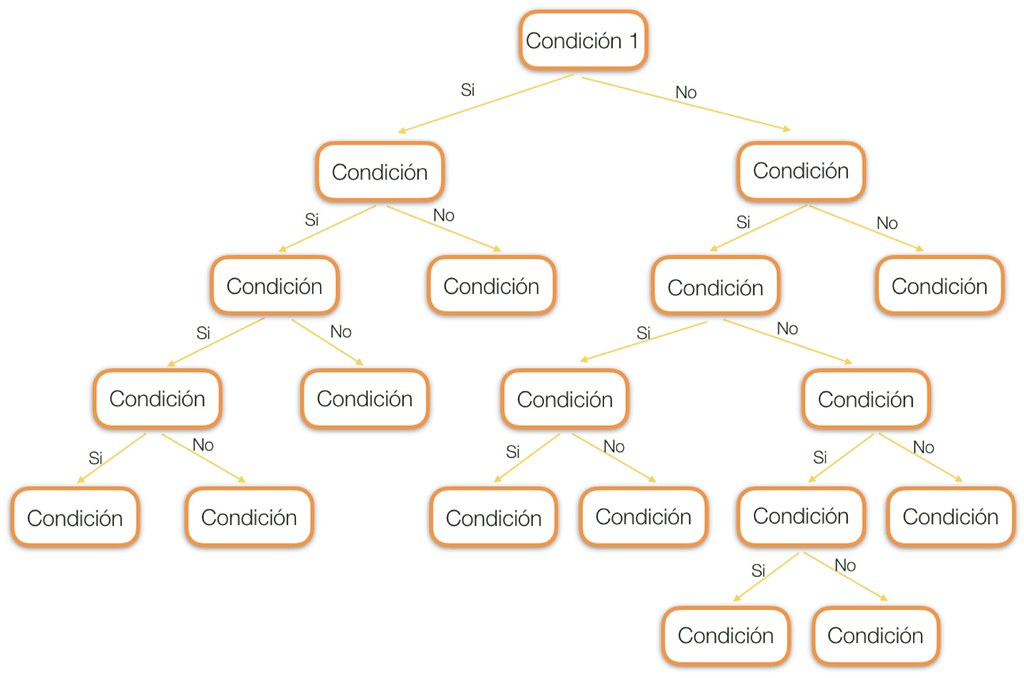
\includegraphics[width=\textwidth]{img/estructura-arbol-de-decision.jpg}        
    \end{minipage}

    \begin{minipage}[t]{0.9\textwidth}
        Fuente: Aprende IA. Recuperado de \url{https://aprendeia.com/arboles-de-decision-clasificacion-teoria-machine-learning/}
    \end{minipage}
\end{figure}

En la figura anterior se puede visualizar la estructura que posee un árbol de decisión, en este se aprecia como actua el algoritmo de partición binaria mencionado al comienzo, tomando un conjunto y separandolo en subconjuntos hasta llegar a un final previamente establecido.

Para estimar la precisión de un clasificador, se calcula la tasa de error de clasificación verdadera. Esta tasa se obtiene evaluando un conjunto de valores X a los que el clasificador asigna una clase incorrecta, y se divide por el total de valores en X. Idealmente, se debería conocer la clase de todos los casos en el universo antes del entrenamiento, o en su defecto, de una muestra de tamaño similar al universo. Sin embargo, en la mayoría de los casos reales, no se dispone de todos los datos del universo, por lo que se trabaja con una muestra y se estima la tasa de error mencionada anteriormente utilizando \emph{estimadores internos}.

\begin{itemize}
    \item \textbf{Ventajas de los árboles de decisión}
    \begin{itemize}
        \item \textbf{Interpretabilidad:} Los árboles de decisión son fácilmente interpretables y comprensibles para los humanos. La estructura del árbol se puede visualizar de manera intuitiva, lo que permite comprender cómo se toman las decisiones y qué atributos son más relevantes para la clasificación.
        \item \textbf{Facilidad de uso:} La construcción y el uso de un árbol de decisión son relativamente sencillos en comparación con otros algoritmos de aprendizaje automático más complejos. No requieren una preparación exhaustiva de los datos ni un procesamiento previo complicado. Además, los árboles de decisión pueden manejar datos numéricos y categóricos sin requerir transformaciones adicionales, lo que simplifica el flujo de trabajo de modelado.
        \item \textbf{Capacidad para manejar datos faltantes y variables irrelevantes:} Los árboles de decisión tienen la capacidad de manejar datos faltantes en los atributos de forma natural. Durante la construcción del árbol, si un atributo tiene valores faltantes, el modelo puede utilizar otros atributos para tomar decisiones sin requerir imputación de datos. Además, los árboles de decisión son resistentes a variables irrelevantes, lo que significa que pueden ignorar atributos que no aportan información útil para la clasificación.
        \item \textbf{Flexibilidad y robustez:} Los árboles de decisión pueden manejar tanto problemas de clasificación como de regresión. Además, son capaces de capturar relaciones no lineales entre los atributos y la variable objetivo. Aunque cada árbol individual puede ser susceptible al sobreajuste, se pueden aplicar técnicas de regularización, como la poda, para mejorar la generalización y evitar el sobreajuste.
        \item \textbf{Eficiencia en tiempo de entrenamiento y predicción:} Los árboles de decisión tienen tiempos de entrenamiento y predicción rápidos, ya que solo implican la evaluación de una serie de reglas de decisión. Aunque el tiempo de construcción puede ser mayor para conjuntos de datos grandes, una vez construido, el árbol puede ser utilizado eficientemente para hacer predicciones en tiempo real.
    \end{itemize}
    \item \textbf{Desventajas de los árboles de decisión}
    \begin{itemize}
        \item \textbf{Sensibilidad a cambios pequeños en los datos:} Los árboles de decisión son muy sensibles a cambios pequeños en los datos de entrenamiento. Una modificación mínima en los datos de entrada puede dar lugar a un árbol de decisión completamente diferente. Esto puede hacer que el modelo sea inestable y su rendimiento pueda variar significativamente.
        \item \textbf{Tendencia al sobreajuste:} Los árboles de decisión tienen la capacidad de adaptarse demasiado a los datos de entrenamiento. Si no se controla adecuadamente, el árbol puede memorizar el ruido o las fluctuaciones aleatorias en los datos de entrenamiento, lo que puede resultar en un mal rendimiento en datos nuevos y no vistos. La poda y otras técnicas de regularización se utilizan para mitigar este problema.
        \item \textbf{Limitaciones en la representación de relaciones complejas:} Aunque los árboles de decisión pueden capturar relaciones no lineales entre atributos y la variable objetivo, pueden tener dificultades para representar relaciones complejas que requieren una combinación de múltiples atributos. Las decisiones tomadas en cada nodo se basan en un solo atributo, lo que puede limitar su capacidad para modelar interacciones más sofisticadas.
        \item \textbf{Propensión a sesgos en los datos de entrenamiento:} Los árboles de decisión pueden verse afectados por sesgos en los datos de entrenamiento, especialmente cuando hay desequilibrios en las clases o falta representación de ciertas categorías. Esto puede resultar en una clasificación desigual o inexacta en casos minoritarios o poco representados.
    \end{itemize}
\end{itemize}

\subsubsection{Modelo Random Forest}
\\
El algoritmo random forest corresponde a un algoritmo empleado en machine learning registrado por Leo Breiman y Adele Cutler \cite{random-forest}, este combina la salida de múltiples árboles de decisión para llegar a un resultado. El uso de random forest se ha hecho popular a causa de su facilidad de uso y flexibilidad, ya que puede ser empleado para problemas de clasificación y regresión.

El random forest se encuentra formado por varios árboles de decisión, los cuales son propensos a tener problemas como sesgos o sobreajuste, pero cuando se trata con una gran cantidad de árboles se logra llegar a resultados más precisos. ''Mientras que los árboles de decisión consideran todas las posibles divisiones de características, los bosques aleatorios solo seleccionan un subconjunto de esas características.'' \cite{random-forest}

Random forest cuenta con tres hiperparámetros principales que se deben de configurar antes de iniciar el entrenamiento \cite{random-forest}:

\begin{itemize}
    \item Tamaño del nodo.
    \item Cantidad de árboles de decisión.
    \item Cantidad de características muestreadas. 
\end{itemize}

El algoritmo se encuentra compuesto de un conjunto de árboles de decisión, cada árbol del conjunto se encuentra compuesto de una muestra de datos, la cual proviene de un conjunto de entrenamiento con reemplazo, llamada muestra de arranque \cite{random-forest}.

A partir de la muestra de entrenamiento, se extrae un porcentaje para reservarlos como datos de prueba, los cuales se conocen como muestra fuera de la bolsa (oob). Luego, se inyecta otra instancia de aleatoriedad mediante el agrupamiento de características, lo que agrega más diversidad al conjunto de datos y reduce la correlación entre los árboles de decisión \cite{random-forest}.

En un Random Forest, el proceso de predicción puede variar según el tipo de problema que se esté abordando \cite{random-forest}. En el caso de tareas de regresión, se utiliza un enfoque de promediado, donde las predicciones de los árboles de decisión individuales se promedian para obtener el valor final de la predicción. Esto proporciona una estimación más precisa y estable del resultado deseado. Por otro lado, en tareas de clasificación, se utiliza un enfoque de votación mayoritaria. Cada árbol de decisión emite su propia predicción y la clase que obtiene la mayoría de votos se selecciona como la clase predicha. Esto permite tomar una decisión conjunta basada en las opiniones de múltiples árboles, lo que puede mejorar la precisión en la clasificación de las muestras.

Finalmente, la muestra extraída en un comienzo, la muestra fuera de la bolsa (oob) será utilizada para realizar una validación cruzada, finalizando la predicción.

\begin{figure}[H]
    \begin{minipage}[t]{0.9\textwidth}
        \caption{Estructura de un random forest}
        \label{random-forest}        
    \end{minipage}

    \vspace{10pt}

    \begin{minipage}[b]{1.1\textwidth}
        \centering
        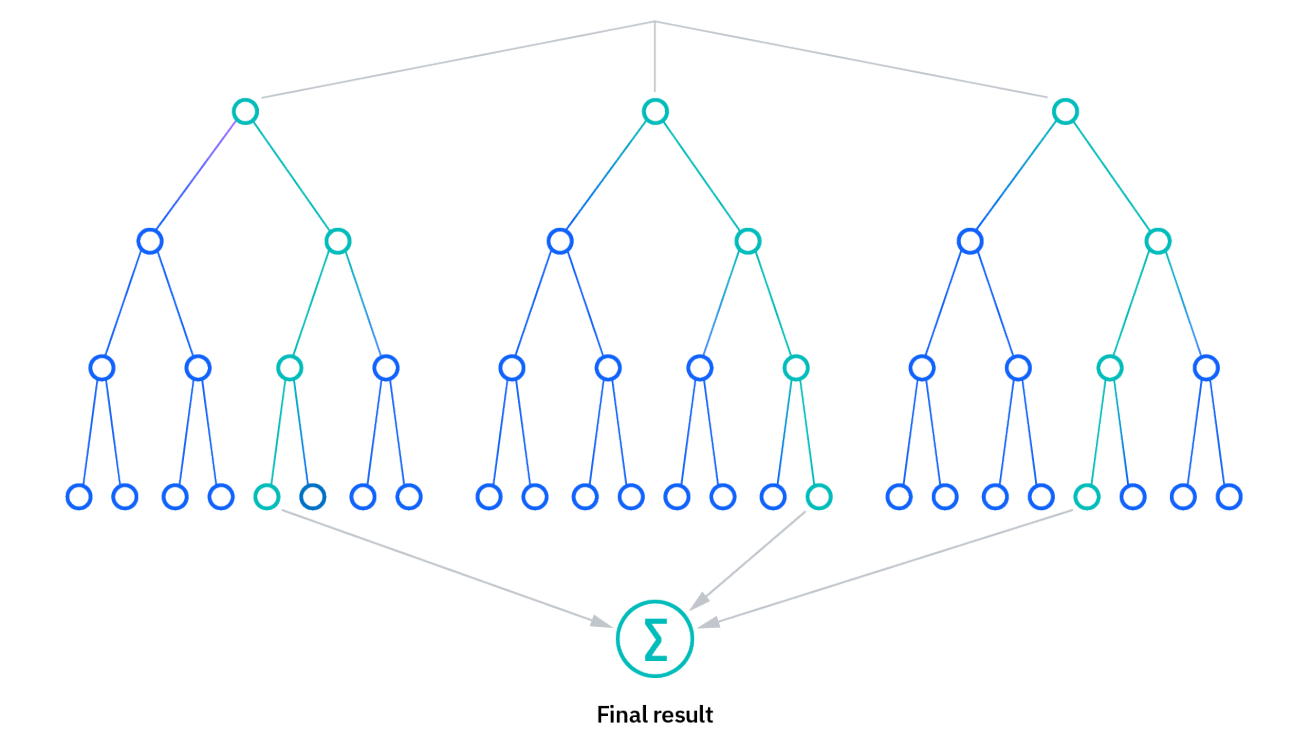
\includegraphics[width=\textwidth]{img/estructura-random-forest.png}        
    \end{minipage}

    \begin{minipage}[t]{0.9\textwidth}
        Fuente: IBM. Recuperado de \url{https://www.ibm.com/mx-es/topics/random-forest}
    \end{minipage}
\end{figure}

\begin{itemize}
    \item \textbf{Ventajas de random forest}
    \begin{itemize}
        \item \textbf{Riesgo reducido de sobreajuste:} Los árboles de decisión corren el riesgo de sobre ajustarse, ya que tienden a ajustar todas las muestras que se encuentran dentro de los datos de entrenamiento. Sin embargo, cuando hay una gran cantidad de árboles de decisión dentro del random forest, el clasificador no será capaz de ajustarse demasiado al modelo, ya que el promedio de los árboles no correlacionados logra reducir la varianza general y el error de predicción.
        \item \textbf{Aporta Flexibilidad:} Debido a su capacidad para abordar con gran precisión tanto tareas de regresión como de clasificación, el método conocido como random forest es ampliamente utilizado por los científicos de datos. Además, su capacidad de agrupar características lo convierte en una herramienta eficaz para estimar valores faltantes, manteniendo la precisión incluso cuando falta parte de los datos.
        \item \textbf{Importancia de la característica fácil de determinar:} El random forest ofrece una forma conveniente de evaluar la importancia o contribución de las variables en un modelo. Existen varias formas de medir la importancia de las características. Por lo general, se utilizan el índice de Gini y la disminución media de impurezas (MDI) para evaluar cuánto afecta la exclusión de una variable específica a la precisión del modelo.
        Sin embargo, otra medida de importancia es la importancia de permutación, también conocida como precisión de disminución media (MDA). La MDA determina la disminución promedio en la precisión al permutar de forma aleatoria los valores de las características en las muestras out-of-bag (muestras que no se utilizan en el proceso de entrenamiento).
    \end{itemize}
    \item \textbf{Desventajas de random forest}
    \begin{itemize}
        \item \textbf{Proceso que requiere mucho tiempo:} Debido a que los algoritmos de random forest son capaces de manejar conjuntos de datos extensos, suelen ofrecer predicciones más precisas. Sin embargo, es importante tener en cuenta que el procesamiento de datos puede volverse lento, ya que se deben calcular los datos para cada árbol de decisión de forma individual.  
        \item \textbf{Requiere más recursos:} Debido a que los random forest procesan conjuntos de datos más grandes, es cierto que se requieren más recursos para almacenar dichos datos. El aumento en el tamaño del conjunto de datos implica una mayor necesidad de memoria y capacidad de almacenamiento para garantizar un funcionamiento eficiente del algoritmo.    
        \item \textbf{Más Complejo:} La interpretación de la predicción de un solo árbol de decisiones resulta más sencilla en comparación con la interpretación de un conjunto de árboles de decisión.
    \end{itemize}
\end{itemize}

\subsubsection{Autoencoders de Redes LSTM para Predicción de Comportamiento de Usuario}
Los autoencoders de redes LSTM son una fusión de dos conceptos poderosos en el aprendizaje profundo: autoencoders y redes neuronales LSTM. Los autoencoders son una clase de redes neuronales utilizadas para la codificación de características; esencialmente, aprenden una representación comprimida de los datos de entrada, que luego pueden ser utilizados para reconstruir la entrada original. Esto es especialmente útil para reducir la dimensionalidad de los datos y descubrir relaciones latentes.

Las redes LSTM son una variante de las redes neuronales recurrentes (RNN) diseñadas para recordar información durante periodos extensos y son particularmente eficientes en el manejo de secuencias de datos con dependencias a largo plazo. Las RNN tradicionales luchan con el aprendizaje de estas dependencias debido al problema del desvanecimiento del gradiente, donde la información se pierde en cada paso a través del tiempo. Las LSTM abordan este problema con una estructura de celdas que incluye compuertas para regular el flujo de información, permitiendo que la red retenga o descarte datos a través de secuencias largas.

Al combinar ambos, los autoencoders LSTM pueden aprender a comprimir secuencias de datos temporales y, a la vez, capturar las complejidades de las secuencias temporales. Esto los hace idóneos para tareas como la predicción del comportamiento del usuario en canales web, donde es crucial comprender y actuar sobre patrones a lo largo del tiempo. Por ejemplo, pueden identificar secuencias de clics que conducen a una compra o predecir cuándo un usuario está a punto de abandonar una sesión, permitiendo intervenir en tiempo real para mejorar la experiencia del usuario y aumentar la conversión.

En un canal web, donde cada acción del usuario es parte de una secuencia más grande de interacciones, los autoencoders LSTM pueden procesar esta secuencia como un todo cohesivo, identificando patrones en la forma en que los usuarios interactúan con el sitio. Esto va más allá de mirar eventos individuales aislados y permite a los sistemas de recomendación anticipar necesidades o intereses futuros basándose en el comportamiento previo del usuario.

\subsubsection{Ventajas de los Autoencoders de Redes LSTM}
\begin{itemize}
        \item \textbf{Aprendizaje de secuencias temporales:} Los autoencoders LSTM son inherentemente buenos en aprender dependencias a largo plazo en datos secuenciales, lo que los hace ideales para rastrear y predecir el comportamiento del usuario en un sitio web a lo largo del tiempo.
        \item \textbf{Reducción de dimensionalidad:}  Los autoencoders son eficaces para comprimir la información y resaltar características latentes, facilitando el manejo de grandes volúmenes de datos de usuario y su posterior análisis.
        \item \textbf{Capacidad de generalización:} Pueden generalizar aprendizajes a partir de datos históricos para predecir acciones futuras, lo que puede mejorar la personalización de contenidos y ofertas en un canal web.
        \item \textbf{Robustez frente al ruido:} Los LSTM pueden manejar el ruido en los datos de entrada, como sesiones de navegación erráticas o inusuales, identificando patrones consistentes y relevantes.
\end{itemize}

\subsubsection{Desventajas de los Autoencoders de Redes LSTM}
\begin{itemize}
        \item \textbf{Complejidad computacional:} Los LSTM son modelos complejos que requieren una mayor capacidad de cómputo, lo que puede traducirse en un procesamiento más lento y costos más elevados.
        \item \textbf{Dificultad en el ajuste de parámetros:} La configuración de estos modelos es a menudo menos intuitiva que otros métodos más simples, lo que puede llevar a un proceso de ajuste laborioso.
        \item \textbf{Riesgo de sobreajuste:} A pesar de su capacidad para generalizar, los LSTM pueden sobreajustarse a los datos de entrenamiento si no se implementan adecuadamente técnicas de regularización.
        \item \textbf{Sensibilidad a los datos de entrenamiento:} Los autoencoders LSTM aprenden de los datos disponibles, lo que significa que cualquier sesgo en estos puede llevar a recomendaciones sesgadas o irrelevantes.
\end{itemize}

\subsection{Tabla comparativa de los modelos de predicción}
La tabla comparativa proporciona información sobre los modelos planteados anteriormente, presentando de forma resumida sus Ventajas, Desventajas y Aplicaciones comunes de los modelos. Permitiendo tener una visión general de las características y consideraciones clave de cada modelo.

\begin{table}[ht]
\captionsetup{font=small} % Ajusta el tamaño de fuente de la leyenda de la tabla
\small % Ajusta el tamaño de fuente de la tabla
\begin{tabular}{|p{0.2\linewidth}|p{0.27\linewidth}|p{0.27\linewidth}|p{0.26\linewidth}|}
\hline
\textbf{Modelo} & \textbf{Ventajas} & \textbf{Desventajas} & \textbf{Aplicaciones} \\
\hline
Modelos de Regresión & 
Proporciona una relación cuantitativa entre variables independientes y la variable de respuesta. & 
Supone una relación lineal entre variables, lo que puede no ser válido en todos los casos. & 
Predicción de valores numéricos continuos. \\
\hline
Modelos de Recomendación & 
Personalización de sugerencias para los usuarios. & 
Puede requerir una gran cantidad de datos y tener problemas con datos faltantes o sesgos inherentes. & 
Recomendaciones de productos en comercio electrónico. \\
\hline
Modelos de Series Temporales & 
Captura patrones temporales y estacionales en los datos a lo largo del tiempo. & 
Sensibilidad a valores atípicos y datos faltantes, y dificultad para capturar tendencias no lineales. & 
Predicción de la demanda de productos. Pronóstico del clima. \\
\hline
Modelos de Atribución & 
Permite cuantificar la contribución relativa de diferentes variables a un resultado o impacto. & 
Puede ser difícil determinar la verdadera relación causal entre las variables. & 
Evaluación del retorno de inversión (ROI) de una campaña publicitaria. \\
\hline
Modelos de Árboles de Decisión & 
Proporciona una estructura de decisiones fácilmente interpretable. & 
Pueden ser propensos al sobreajuste si no se controla adecuadamente. & 
Clasificación y predicción en diversos campos, como medicina, marketing y finanzas. \\
\hline
Modelo Random Forest & 
Combina múltiples árboles de decisión para mejorar la precisión y evitar el sobreajuste. & 
Puede ser computacionalmente costoso y más difícil de interpretar que un solo árbol de decisión. & 
Clasificación y predicción en una amplia gama de aplicaciones, como análisis de datos médicos y detección de fraudes. \\
\hline
\end{tabular}
\end{table}


\subsection{Series Temporales}
Luego de realizar distintas investigaciones, hemos llegado a la certeza de que serán necesarios los modelos basados en series temporales. Se llego a esta decisión debido que se busca predecir el comportamiento futuro de los clientes, en base a su ruta de navegación pasada. A continuación se abarcaran las distintas propiedades de series temporales y sus graficos, además, se presentaran 3 modelos ampliamente aplicados en series temporales, los cuales son, el modelo ARIMA, SARIMA y redes LSTM:
\subsubsection{Graficos de series temporales}
Uno de los primeros pasos para poder realizar cualquier tipo de análisis de datos es necesario graficar los datos, los gráficos permiten ver las distintas propiedades que los datos puedan tener, como lo son patrones, observaciones inusuales (outliers), cambios producidos por el tiempo y las relaciones que se encuentran entre las distintas variables que los datos puedan tener \cite{forecast-time-series-arima}. Por lo que, la selección de un buen grafico para representar los datos resulta ser de gran importancia para poder seleccionar el modelo predictivo más adecuado.

Dentro de esta sección revisaremos los gráficos más relevantes para nuestro estudio:


\begin{itemize}
    \item \textbf{Trama de tiempo (Time plot):} Una de las maneras más practicas y usada para poder entender las series de tiempo es graficar los datos y una de las primeras opciones es una trama de tiempo. Esto quiere decir graficar la datos contra el tiempo de obtención de los datos.
    
    La siguiente figura muestra la cantidad semanal de pasajeros que volaron en la clase económica de Ansett Airlines entre las dos ciudades más grandes de Australia \cite{forecast-time-series-arima}:

    \begin{figure}[H]
        \begin{minipage}[t]{0.9\textwidth}
            \caption{Cantidad semanal de pasajeros que volaron en la clase económica de Ansett Airlines}
            \label{timeplot}        
        \end{minipage}
    
        \vspace{10pt}
    
        \begin{minipage}[b]{1.1\textwidth}
            \centering
            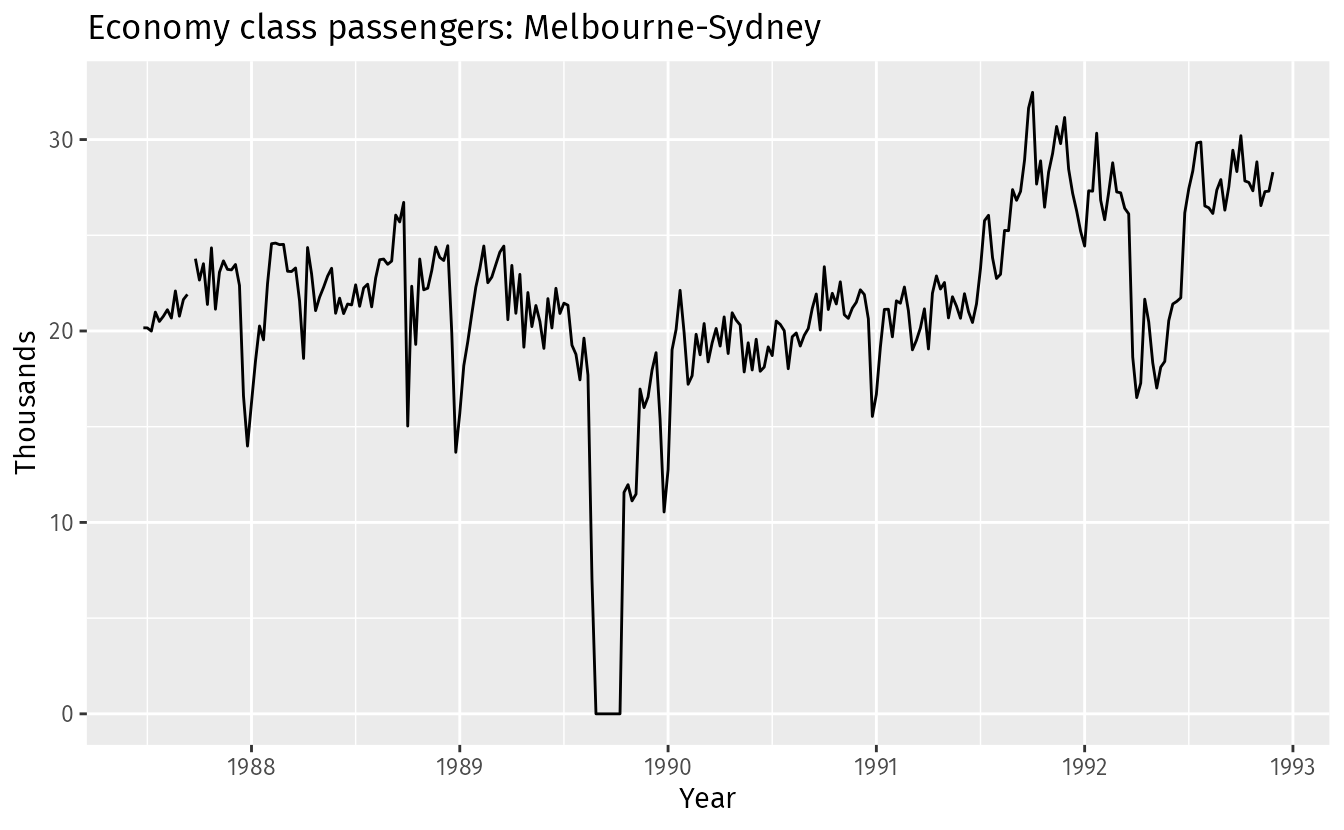
\includegraphics[width=\textwidth]{img/pasajeros-clase-econ-timeplot.png}        
        \end{minipage}
    
        \begin{minipage}[t]{0.9\textwidth}
            Fuente: Forecasting: Principles and Practice (Hyndman y Athanasopoulos, 2023). Recuperado de \url{https://otexts.com/fpp2/time-plots.html}
        \end{minipage}
    \end{figure}
    
    \item \textbf{Patrónes:} Una serie de tiempo puede presentar distintos tipos de patrones a lo largo del tiempo de la observación, y estos patrones son:
        \begin{itemize}
            \item Tendencia (Trend):
            \item Estacional (Seasonal):
            \item Cíclico (Cyclic):
        \end{itemize}

        Muchas veces nos encontraremos con series de tiempo que contienen uno o más de estos patrones, por lo que para poder elegir un método predictivo resulta imperativo identificar los patrones presentes en los datos \cite{forecast-time-series-arima}.

    \item \textbf{Tramas de tiempo estacionales (Seasonal plots):} Esta grafica es similar a la trama de tiempo antes mencionada, la diferencia reside en el hecho de que los datos u observaciones están graficadas en contra de cada “estación individual” de tiempo donde se realizó la observación \cite{forecast-time-series-arima}.
    
        En la siguiente figura se representa el valor monetario de las ventas mensuales de medicamentos antidiabéticos en Australia:
        
        \begin{figure}[H]
            \begin{minipage}[t]{0.9\textwidth}
                \caption{Ventas mensuales de medicamentos antidiabéticos en Australia}
                \label{seasonalplot}        
            \end{minipage}
        
            \vspace{10pt}
        
            \begin{minipage}[b]{1.1\textwidth}
                \centering
                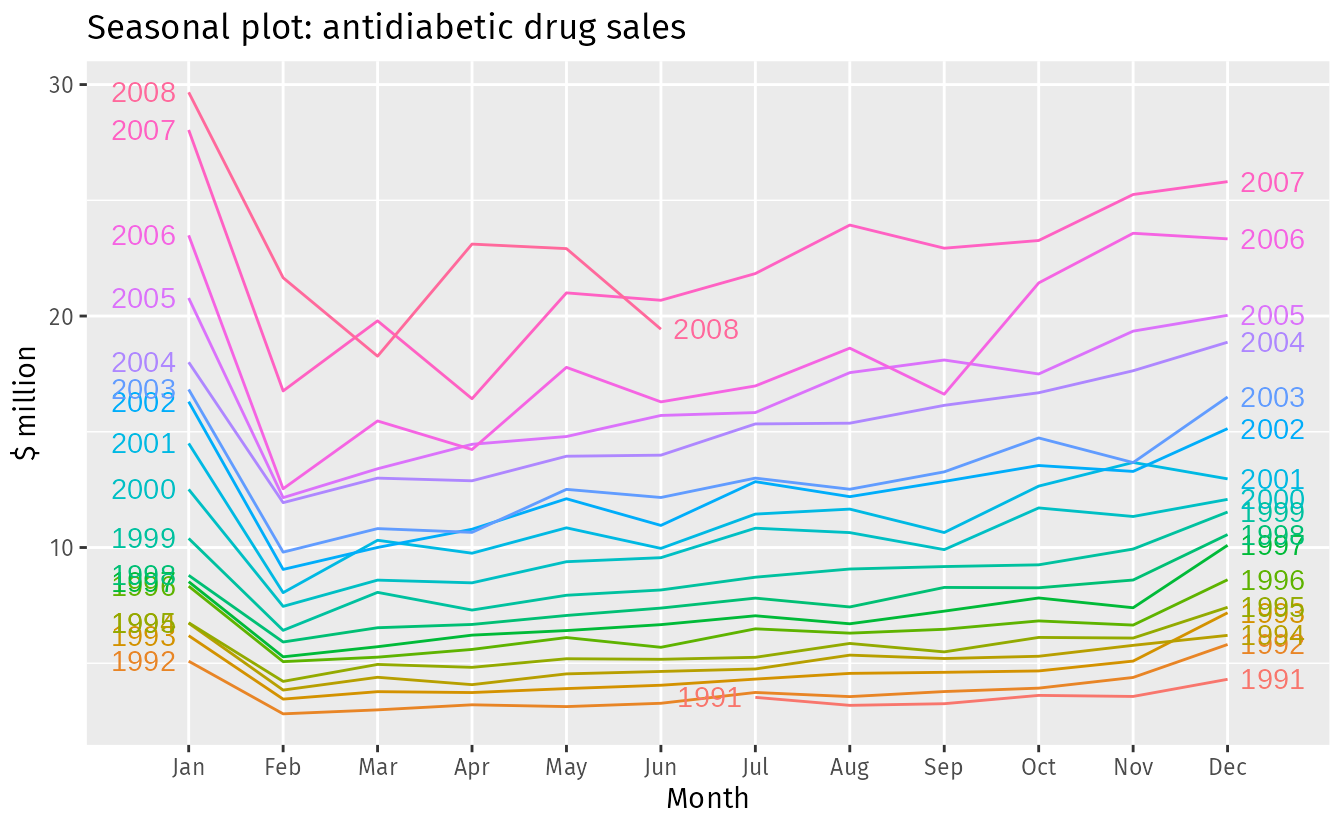
\includegraphics[width=\textwidth]{img/ventas-medicamentos-diab-seasonplot.png}        
            \end{minipage}
        
            \begin{minipage}[t]{0.9\textwidth}
                Fuente: Forecasting: Principles and Practice (Hyndman y Athanasopoulos, 2023). Recuperado de \url{https://otexts.com/fpp2/time-plots.html}
            \end{minipage}
        \end{figure}

        Este tipo de gráficos permite identificar de mejor manera los patrones que no se pudieron apreciar anteriormente en la trama de tiempo, ayuda especialmente para poder observar en que años el patrón de los datos cambia.

    \item \textbf{Gráficos de dispersión (Scatterplots):} Este tipo de grafico permite explorar las relaciones que existen entre series de tiempo, sus distintas variables y como esto afecta a la hora de predecir una serie de tiempo.

        La siguiente figura muestra dos series de tiempo: demanda de electricidad (en GW y temperatura (Celsius)), para 2014 en Victoria, Australia. Las temperaturas son para Melbourne, la ciudad más grande de Victoria, mientras que los valores de demanda son para todo el estado \cite{forecast-time-series-arima}.

        \begin{figure}[H]
            \begin{minipage}[t]{0.9\textwidth}
                \caption{Demanda electrica debido a las temperaturas en 2 ciudades en Australia}
                \label{scatteroplot}        
            \end{minipage}
        
            \vspace{10pt}
        
            \begin{minipage}[b]{1.1\textwidth}
                \centering
                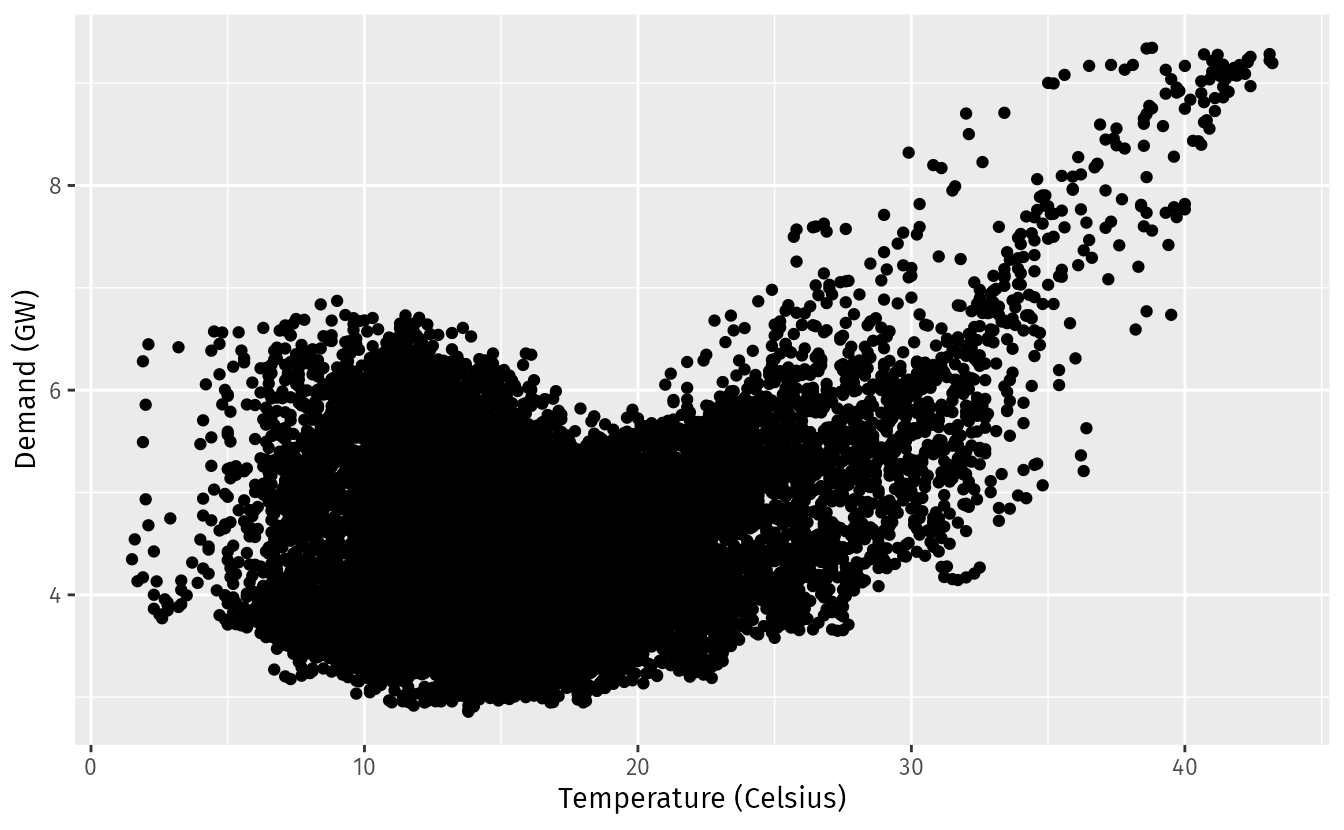
\includegraphics[width=\textwidth]{img/Demanda electrica debido a las temperaturas en 2 ciudades en Australia.png}        
            \end{minipage}
        
            \begin{minipage}[t]{0.9\textwidth}
                Fuente: Forecasting: Principles and Practice (Hyndman y Athanasopoulos, 2023). Recuperado de \url{https://otexts.com/fpp2/time-plots.html}
            \end{minipage}
        \end{figure}

        Este grafico de dispersión es de gran ayuda para visualizar la relación que tienen las variables, y poder entender los datos de mejor manera.

    \item \textbf{Gráficos de desfase (Lag plots):} Este tipo de gráfico representa la observación Y(t) graficada contra la observación Y(t-k) para cada valor de k. Donde en el eje horizontal se muestran valores desfasados de la serie de tiempo \cite{forecast-time-series-arima}. La siguiente figura muestra diagramas de dispersión de la producción trimestral de cerveza australiana:
    
    \begin{figure}[H]
        \begin{minipage}[t]{0.9\textwidth}
            \caption{Producción trimestral de cerveza australiana}
            \label{lagplot}        
        \end{minipage}
    
        \vspace{10pt}
    
        \begin{minipage}[b]{1.1\textwidth}
            \centering
            \includegraphics[width=\textwidth]{img/producción trimestral de cerveza australiana-lagplot.png}        
        \end{minipage}
    
        \begin{minipage}[t]{0.9\textwidth}
            Fuente: Forecasting: Principles and Practice (Hyndman y Athanasopoulos, 2023). Recuperado de \url{https://otexts.com/fpp2/time-plots.html}
        \end{minipage}
    \end{figure}
    
    Los colores representan el cuatrimestre de la variable en el eje vertical. Se puede apreciar que en los desfases 4 y 8 se presenta una fuerte relación de las variables, lo que muestra un patrón estacional fuerte. 

    \item \textbf{Correlación:} El estudio de la correlación explora la relación lineal entre dos variables, resulta de importancia calcularla, esto debido a que entrega que tan intrínsecamente relacionadas se encuentran las variables a analizar \cite{forecast-time-series-arima}. 
    
    A continuación, se presenta la fórmula para conocer el coeficiente de correlación entre dos variables, x e y:

    \begin{equation*}
        r = \frac{\sum{(x_t - \bar{x})(y_t - \bar{y})}}{{\sqrt{\sum{(x_t - \bar{x})}}\sqrt{\sum{(y_t - \bar{y})}}}}
    \end{equation*}    
    
    El valor de r variara entre -1 y 1, dependiendo de que tan fuerte sea la correlación de las variables, mientras más cercano al -1, r representa una correlación negativa, por lo que, si r se encuentra más cercano a 1, esto quiere decir que las variables tienen una correlación positiva \cite{forecast-time-series-arima}.

    \item \textbf{Autocorrelación:} La autocorrelación mide la relación lineal entre valores rezagados de una serie de tiempo. Hay variados coeficientes de autocorrelación, dependiendo de cada panel del Lag plot, por ejemplo, r1 mide la relación entre las variables Y(t) y Y(t-1) y r2 mide la relación entre las variables Y(t) y Y(t-2) y así hasta considerar todos los datos \cite{forecast-time-series-arima}.
    
    Para calcular el valor de r(k), donde T corresponde al largo de la serie de tiempo., se ocupa la siguiente formula:

    \begin{equation*}
        r_k = \frac{\sum_{t=k+1}^{T}{(y_t - \bar{y})(y_t-k - \bar{y})}}{\sum_{t=1}^{T}(y_t - \bar{y})^2}
    \end{equation*}  

    De ejemplo, se calcularon los primeros 9 coeficientes de autocorrelación de la producción de cerveza en Australia estudiado en la sección pasada, obteniendo los siguientes valores:

    \begin{figure}[H]
        \begin{minipage}[t]{0.9\textwidth}
            \caption{Coeficientes de autocorrelación de la producción de cerveza en Australia}
            \label{autocorrelaciones1}        
        \end{minipage}
    
        \vspace{10pt}
    
        \begin{minipage}[b]{1.1\textwidth}
            \centering
            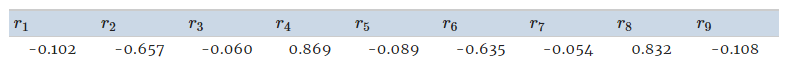
\includegraphics[width=\textwidth]{img/ejemplo_autocorrelaciones.png}        
        \end{minipage}
    
        \begin{minipage}[t]{0.9\textwidth}
            Fuente: Forecasting: Principles and Practice (Hyndman y Athanasopoulos, 2023). Recuperado de \url{https://otexts.com/fpp2/time-plots.html}
        \end{minipage}
    \end{figure}

    Estos coeficientes de autocorrelación son graficados para representar la \textbf{función de autocorrelación (ACF)}, que se muestra a continuación:

    \begin{figure}[H]
        \begin{minipage}[t]{0.9\textwidth}
            \caption{ACF de la produccion trimestral de cerveza}
            \label{autocorrelaciones2}        
        \end{minipage}
    
        \vspace{10pt}
    
        \begin{minipage}[b]{1.1\textwidth}
            \centering
            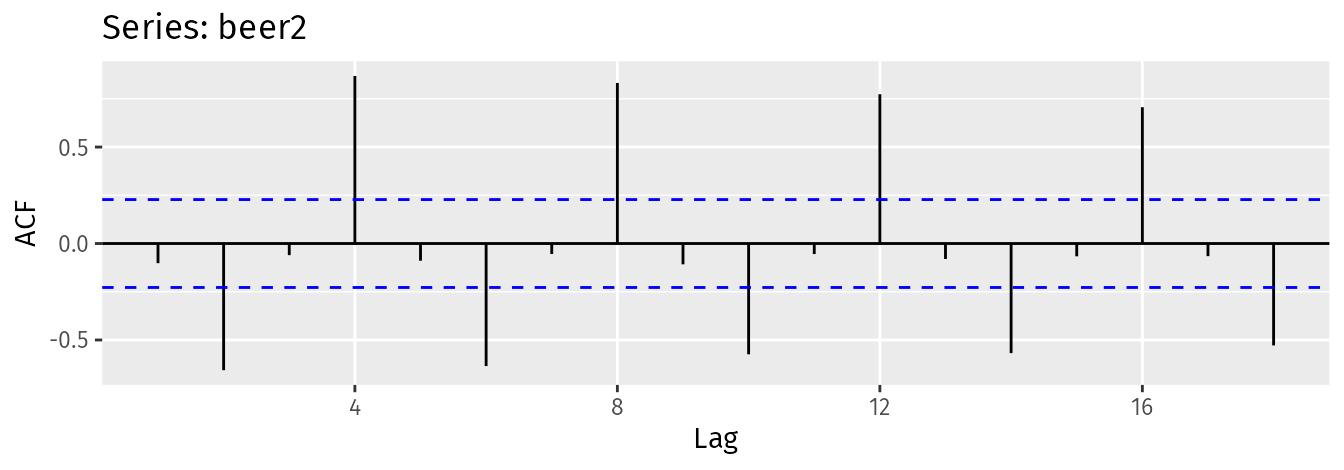
\includegraphics[width=\textwidth]{img/produccion-cerveza-aust-ACF.png}        
        \end{minipage}
    
        \begin{minipage}[t]{0.9\textwidth}
            Fuente: Forecasting: Principles and Practice (Hyndman y Athanasopoulos, 2023). Recuperado de \url{https://otexts.com/fpp2/time-plots.html}
        \end{minipage}
    \end{figure}

    Las líneas azules indican que tan lejos de 0 pueden estar las correlaciones para que estas sean significativas. 
    
    Cuando los datos tienen alguna tendencia, el ACF tiene valores positivos que lentamente van disminuyendo, si los datos presentan un patrón estacional, el ACF mostrara valores más grandes para los desfases estacionales, por lo general siguiendo alguna frecuencia estacional.
    
    Cuando los datos presentan una tendencia y además un patrón estacional, se pueden apreciar ambos efectos \cite{forecast-time-series-arima}. En las siguientes figuras se muestra la demanda mensual de electricidad de Australia, la cual presenta una tendencia y patrón estacional:

    \begin{figure}[H]
        \begin{minipage}[t]{0.9\textwidth}
            \caption{Demanda mensual de electricidad de Australia}
            \label{autocorrelaciones3}        
        \end{minipage}
    
        \vspace{10pt}
    
        \begin{minipage}[b]{1.1\textwidth}
            \centering
            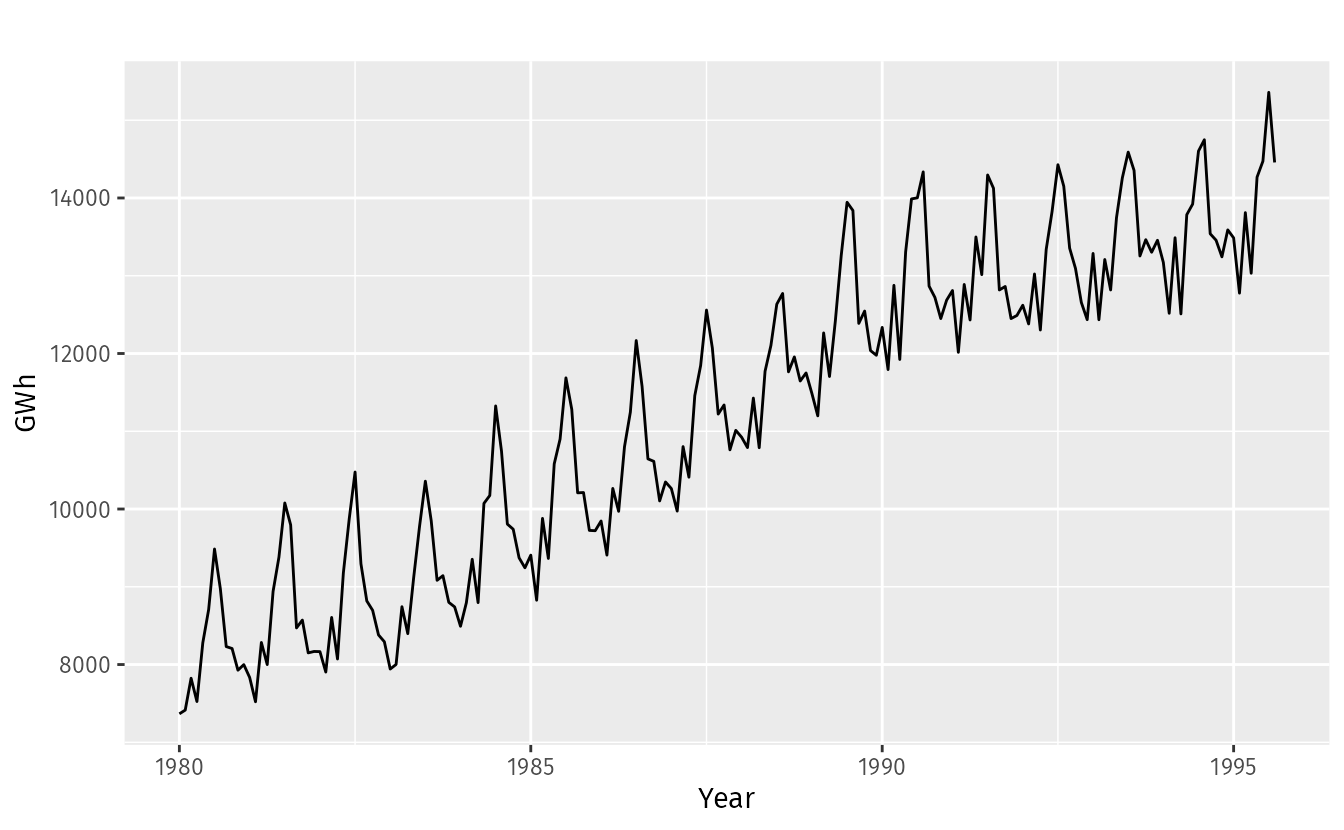
\includegraphics[width=\textwidth]{img/aelec-1-ejemplo.png}        
        \end{minipage}
    
        \begin{minipage}[t]{0.9\textwidth}
            Fuente: Forecasting: Principles and Practice (Hyndman y Athanasopoulos, 2023). Recuperado de \url{https://otexts.com/fpp2/time-plots.html}
        \end{minipage}
    \end{figure}

    \begin{figure}[H]
        \begin{minipage}[t]{0.9\textwidth}
            \caption{ACF demanda mensual de electricidad de Australia}
            \label{autocorrelaciones4}        
        \end{minipage}
    
        \vspace{10pt}
    
        \begin{minipage}[b]{1.1\textwidth}
            \centering
            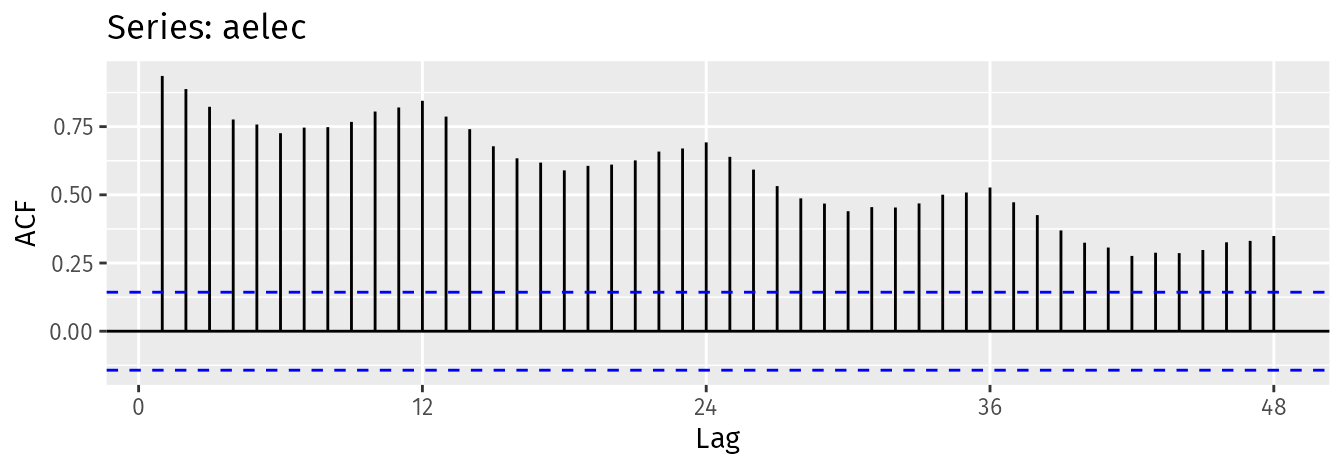
\includegraphics[width=\textwidth]{img/acfelec-1-ejemplo.png}        
        \end{minipage}
    
        \begin{minipage}[t]{0.9\textwidth}
            Fuente: Forecasting: Principles and Practice (Hyndman y Athanasopoulos, 2023). Recuperado de \url{https://otexts.com/fpp2/time-plots.html}
        \end{minipage}
    \end{figure}

    En el ACF se puede apreciar una tendencia, esto debido a que los valores van disminuyendo lentamente, mientras que la forma de ondas es debido a la estacionalidad que se presenta cada año.

    \item \textbf{Ruido Blanco (White Noise):} Las series de tiempo que no tienen autocorrelación son llamadas ruido blanco, para esto se espera que cada autocorrelación sea lo más cercana a 0. Debido a la variación que estos valores pueden tener, por lo que para que una serie de tiempo sea considerada ruido blanco, se espera que el 95\% de sus valores representados en el ACF estén unos limites demarcados por $\pm{2}/\sqrt{T}$, donde T corresponde al largo de la serie de tiempo, estos limites se encuentran representados comúnmente por líneas azules en el ACF. Por consiguiente, si un valor o más se encuentra fuera de los limites o el más del 5\% de los valores estén fuera de los límites, la serie de tiempo en cuestión probablemente no sea ruido blanco.

    \begin{figure}[H]
        \begin{minipage}[t]{0.9\textwidth}
            \caption{Ruido blanco}
            \label{whitenoise1}        
        \end{minipage}
    
        \vspace{10pt}
    
        \begin{minipage}[b]{1.1\textwidth}
            \centering
            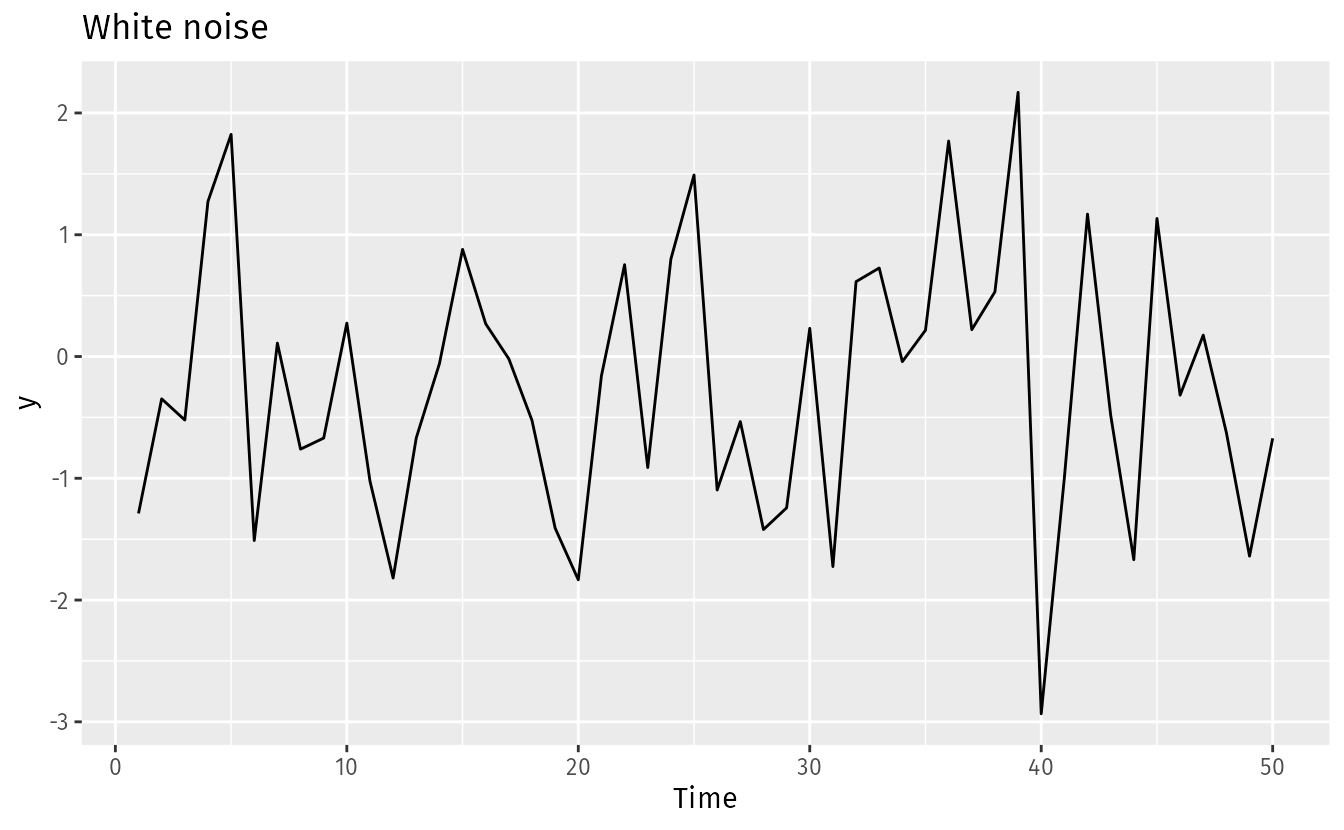
\includegraphics[width=\textwidth]{img/wnoise-1.png}        
        \end{minipage}
    
        \begin{minipage}[t]{0.9\textwidth}
            Fuente: Forecasting: Principles and Practice (Hyndman y Athanasopoulos, 2023). Recuperado de \url{https://otexts.com/fpp2/time-plots.html}
        \end{minipage}
    \end{figure}

    \begin{figure}[H]
        \begin{minipage}[t]{0.9\textwidth}
            \caption{ACF Ruido blanco}
            \label{whitenoise2}        
        \end{minipage}
    
        \vspace{10pt}
    
        \begin{minipage}[b]{1.1\textwidth}
            \centering
            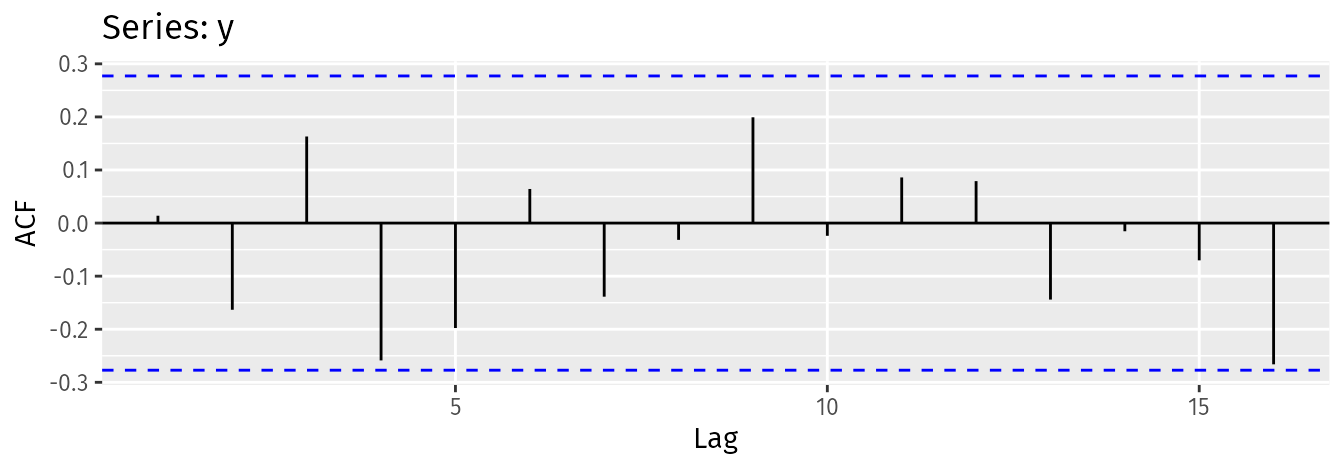
\includegraphics[width=\textwidth]{img/wnoiseacf-1.png}        
        \end{minipage}
    
        \begin{minipage}[t]{0.9\textwidth}
            Fuente: Forecasting: Principles and Practice (Hyndman y Athanasopoulos, 2023). Recuperado de \url{https://otexts.com/fpp2/time-plots.html}
        \end{minipage}
    \end{figure}

    Teniendo en cuenta que T = 50, por lo tanto, los limites están calculados como $\pm{2}/\sqrt{50}  = \pm{0.28}$. En el ACF se puede apreciar que todos los coeficientes de autocorrelación se encuentran dentro estos límites, concluyendo que los datos son ruido blanco.

\end{itemize}


\subsubsection{Modelo ARIMA}
El modelo ARIMA o modelo autorregresivo de media móvil integrado, por sobre otros modelos de series temporales, se centra en describir las autocorrelaciones que existen entre los datos \cite{forecast-time-series-arima}.

\begin{itemize}
    \item \textbf{Estacionariedad:} Una serie de tiempo estacionaria, se presenta cuando sus propiedades no dependen del momento en el que fue registrada la observación. Por lo que, las series de tiempo que presentan tendencias o patrones estacionales son series de tiempo no estacionarias, ya que las tendencias y las distintas estaciones de tiempo pueden afectar la serie de tiempo en varias ocasiones \cite{forecast-time-series-arima}. 
    
    Las series de tiempo estacionarias por lo general son series de ruido blanco, ya que no muestran autocorrelación entre los datos y tampoco presentan patrones predecibles a lo largo del tiempo. 

    \item \textbf{Diferenciación:} Una manera de poder cambiar una seria de tiempo no estacionaria en una estacionaria, es aplicar la diferenciación, esto se refiera a calcular la diferencia entre observaciones consecutivas \cite{forecast-time-series-arima}.
    
    Una de las transformaciones más ocupada para estabilizar la varianza de los datos son los logaritmos. Por otro lado, la diferenciación estabiliza el promedio de la seria de tiempo debido a que es capaz de reducir o remover los distintos cambios que se puedan presentar en la serie de tiempo, tales como las tendencias y patrones estacionales.
    
    \item \textbf{Modelo Random walk:} La serie diferenciada es el cambio que se presenta entre las observaciones consecutivas de la serie original, esta se denota por:
    \begin{equation*}
        y'_t = y_t - y_t-1
    \end{equation*}

    Ya que es imposible conseguir la diferenciada de la primera observación $y'_1$, la serie diferenciada solo tendrá valores T-1. Si la serie diferenciada es un ruido blanco, la fórmula se puede escribir de la siguiente manera, donde $\varepsilon_t$ representa el ruido blanco \cite{forecast-time-series-arima}:
    \begin{equation*}
        y_t-y_t-1= \varepsilon_t
    \end{equation*}

    El \textbf{Modelo Random walk} se obtiene luego de despejar $y_t$:
    \begin{equation*}
        y_t=y_t-1+\varepsilon_t
    \end{equation*}

    Debido a que los movimientos futuros en los datos son impredecibles, las predicciones del modelo son iguales a la ultima observación, por lo que este tipo de modelos es ampliamente ocupado por datos no estacionarios. Pudiendo concluir que el modelo random walk sustenta los pronósticos naïve \cite{forecast-time-series-arima}.

    \begin{equation*} y_t-y_t-1 = C+\varepsilon_t \leftrightarrow y_t=C+y_t-1+\varepsilon_t \end{equation*}

    El valor de C representa el promedio de los cambios entre observaciones consecutivas \cite{forecast-time-series-arima}, dependiendo del signo de C la seria se verá derivada positivamente si es positivo o negativamente en el caso contrario.

    \item \textbf{Diferenciación estacional:} Esta diferenciación se realiza para calcuar el cambio entre una observación y la observación previa de la misma estación de tiempo \cite{forecast-time-series-arima}, obteniendo la siguiente fórmula:
    \begin{equation*}
        y'=y_t-y_t-m
    \end{equation*}

    Donde $m= \text{cantidad de estaciones}$, tambien son llamadas "diferencias $m$-desfazadas", ya que realizamos la resta con una observación luego de $m$ periodos \cite{forecast-time-series-arima}.

    Si luego de realizar una diferenciación estacional a una serie de tiempo, esta parece haberse transformado a ruido blanco, se modelaran los datos originales de la siguiente manera:
    \begin{equation*}
        y_t=y_t-m+\varepsilon_t
    \end{equation*}

    Como este tipo de modelo entrega predicciones iguales a la ultima observación de la estacion seleccionada, en otras palabras, este modelo entrega pronósticos naïve \cite{forecast-time-series-arima}.

    En la siguiente figura se muestra como las diferenciaciones estacionales y la aplicacion de logaritmos a una serie de tiempo, en este caso la venta de medicamentos antidiabéticos, lograr cambiar la forma de la serie a una de ruido \cite{forecast-time-series-arima}:

    \begin{figure}[H]
        \begin{minipage}[t]{0.9\textwidth}
            \caption{Aplicación de logartimos y diferenciación estacional a ventas de medicamentos antidiabéticos}
            \label{seasonaldiff}        
        \end{minipage}
    
        \vspace{10pt}
    
        \begin{minipage}[b]{1.1\textwidth}
            \centering
            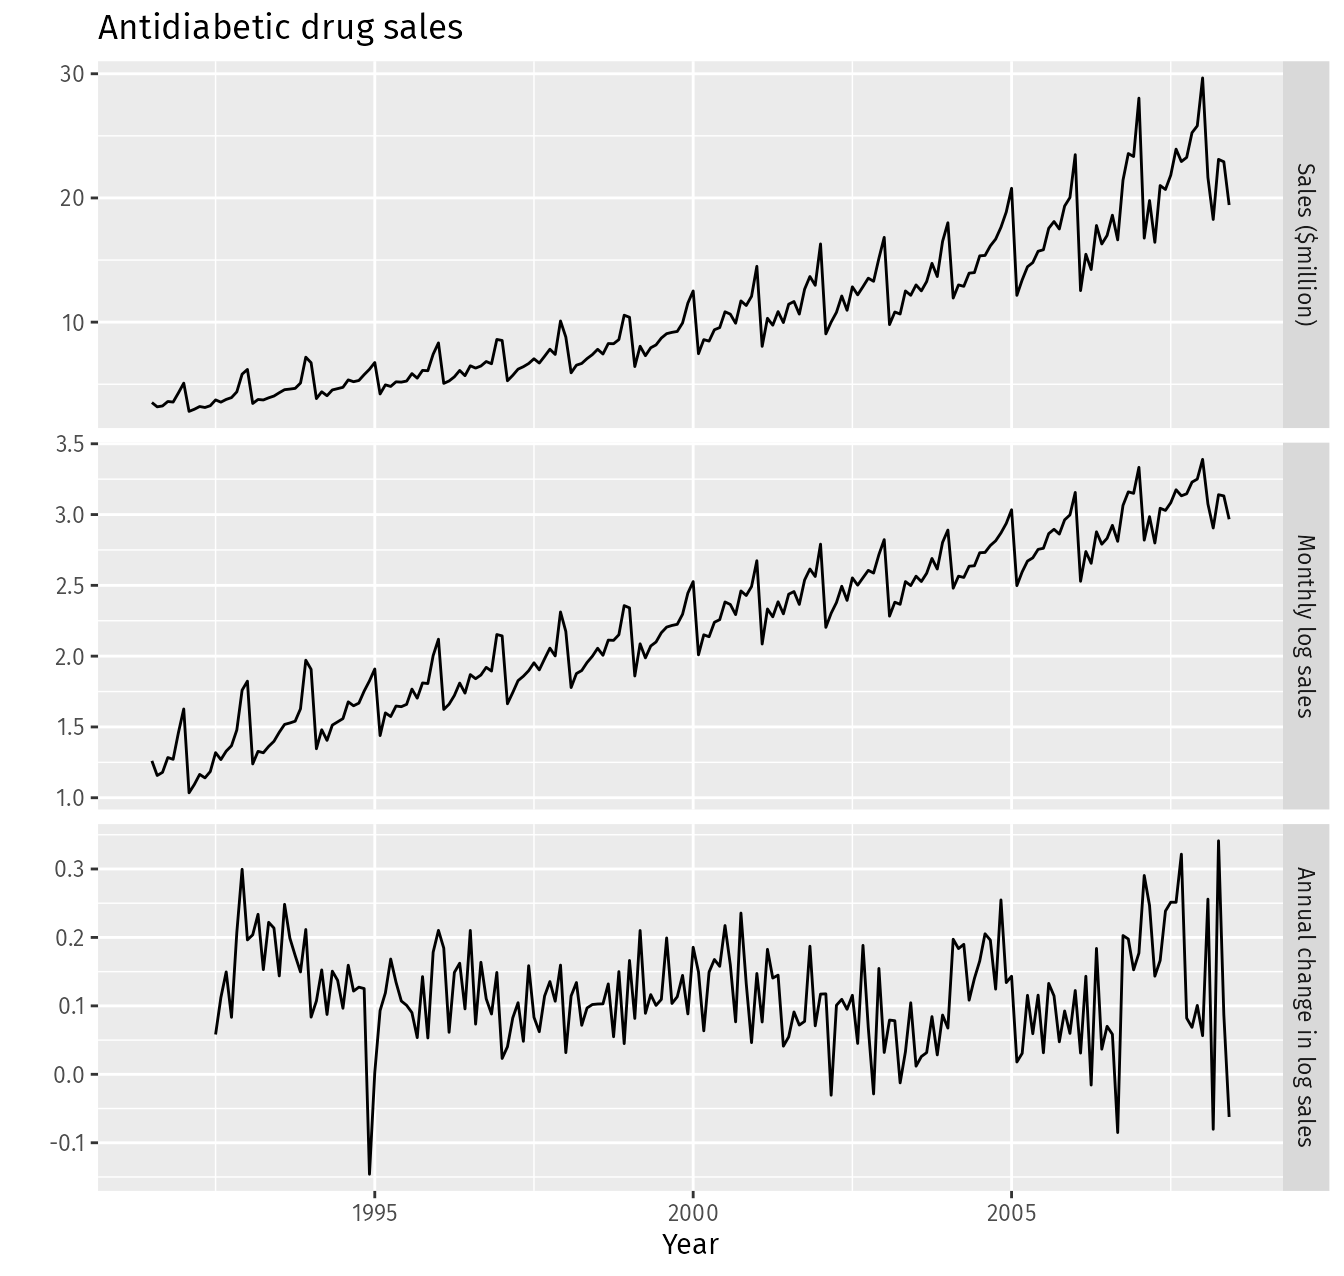
\includegraphics[width=\textwidth]{img/a10diff-1-seasonaldiff-example.png}        
        \end{minipage}
    
        \begin{minipage}[t]{0.9\textwidth}
            Fuente: Forecasting: Principles and Practice (Hyndman y Athanasopoulos, 2023). Recuperado de \url{https://otexts.com/fpp2/time-plots.html}
        \end{minipage}
    \end{figure}

    Por lo general, a la diferenciación ordinaria se le llama "primera diferenciación", refiriendose a las diferenciación en el desfase 1. 
    
    Para poder obtener una serie de tiempo que parezca ruido blanco, muchas veces se tendra que aplicar ambas diferenciaciones, la primera diferenciación y diferenciación estacional, el orden de aplicación no afecta el resultado \cite{forecast-time-series-arima}.
    
    Tambien existe la segunda diferenciada estacional, por lo que el modelo de la serie doblemente diferenciado se escribe de la siguiente manera:
    \begin{equation*}
        y''_t=y'_t-y'_t-1 \leftrightarrow (y_t-y_t-m)-(y_t-1-y_t-m-1) \leftrightarrow y_t-y_t-1-y_t-m+y_t-m-1
    \end{equation*}

    Si la serie de tiempo, presenta un patrón estacional, es recomendable realizar la diferenciación estacional como primer paso para obtener una serie de tiempo estacionaria, pero si se ocupa la primera diferenciación puede que todavia hayan patrones estacionales en la serie de tiempo, teniendo que aplicar más diferenciaciones para obtener la estacionariedad \cite{forecast-time-series-arima}.

    \item \textbf{Modelo de autorregresión:} Como se menciono anteriormente, los modelos autorregresivos predicen la variable de interes utilizando una combinación lineal de valores pasados de la variable. El término autorregresión indica que se trata de una regresión de la variable contra sí misma.
    
    Por lo que un modelo autorregresivo de orden $p$, donde $\varepsilon_t$ corresponde a ruido blanco, se escribe de la siguiente manera:
    \begin{equation*}
        y_t=c+\phi_1y_t-1+\phi_2y_t-2+...+\phi_py_t-p+\varepsilon_t
    \end{equation*}

    Este tipo de modelo es llamado \textbf{AR($p$)}, gracias a la flexibilidad de los modelos autorregresivos, estos pueden ser aplicados en series de tiempo que presenten distintos patrones \cite{forecast-time-series-arima}. A continuación, se presenta una figura que muestran dos modelos AR, AR(1) y AR(2).

    \begin{figure}[H]
        \begin{minipage}[t]{0.9\textwidth}
            \caption{Modelos autorregresivos con diferentes parámetros}
            \label{ARmodel}        
        \end{minipage}
    
        \vspace{10pt}
    
        \begin{minipage}[b]{1.1\textwidth}
            \centering
            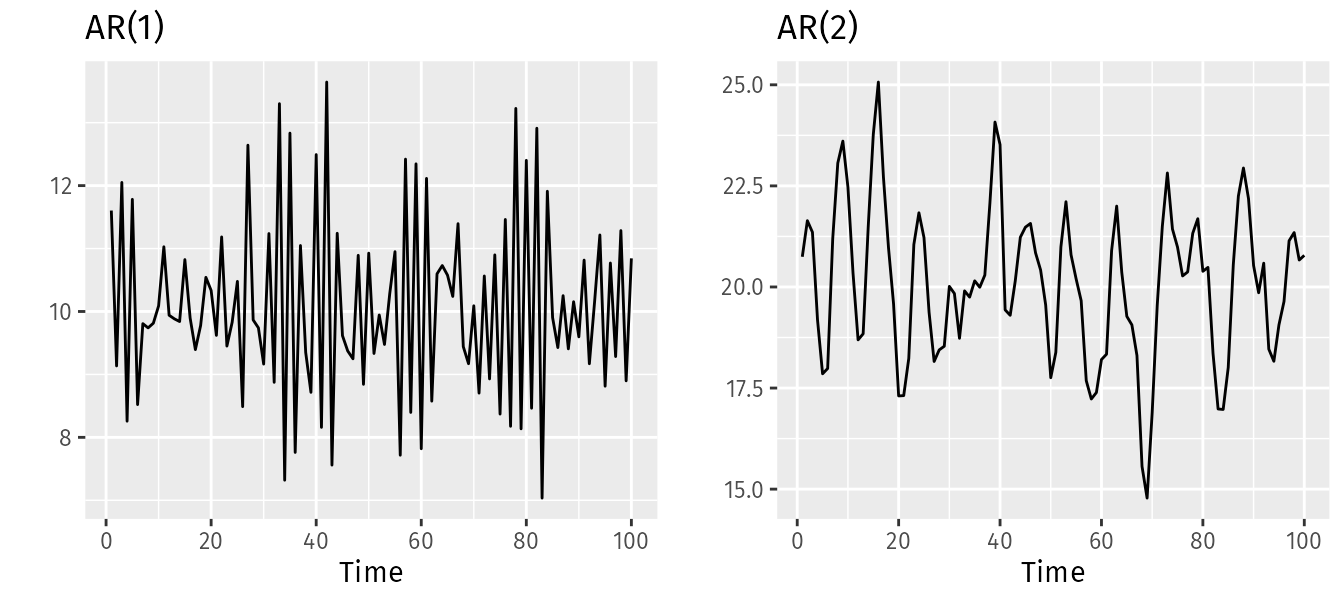
\includegraphics[width=\textwidth]{img/arp-1-example.png}        
        \end{minipage}
    
        \begin{minipage}[t]{0.9\textwidth}
            Fuente: Forecasting: Principles and Practice (Hyndman y Athanasopoulos, 2023). Recuperado de \url{https://otexts.com/fpp2/time-plots.html}
        \end{minipage}
    \end{figure}

    El modelo AR(1) tiene como fórmula: $y_t=18-0.8y_t-1+\varepsilon_t$ y el modelo AR(2) tiene como fórmula: $y_t=8+1.3y_t-1 - 0.7y_t-2+\varepsilon_t$, en ambos casos $\varepsilon_t$ (ruido blanco) tiene una distribución normal, con promedio igual a 0 y varianza igual a 1 \cite{forecast-time-series-arima}.

    \item \textbf{Modelo de media móvil:} Este tipo de modelo ocupa el error de los pronósticos como si fuera un modelo de regresión, con la diferencia en una regresión se ocupan los valores pasados. 

    Teniendo $\varepsilon_t$ como ruido blanco, el modelo de media móvil de orden $q$ o \textbf{MA($q$)} se escribe de la siguiente manera \cite{forecast-time-series-arima}:
    \begin{equation*}
        y_t=c+\varepsilon_t+\theta_1\varepsilon_t-1+\theta_2\varepsilon_t-2+...+\theta_q\varepsilon_t-q+\varepsilon_t
    \end{equation*}

    A continuación, se presenta una figura que muestran dos modelos MA, MA(1) y MA(2).

    \begin{figure}[H]
        \begin{minipage}[t]{0.9\textwidth}
            \caption{Modelos de media móvil con diferentes parámetros}
            \label{MAmodel}        
        \end{minipage}
    
        \vspace{10pt}
    
        \begin{minipage}[b]{1.1\textwidth}
            \centering
            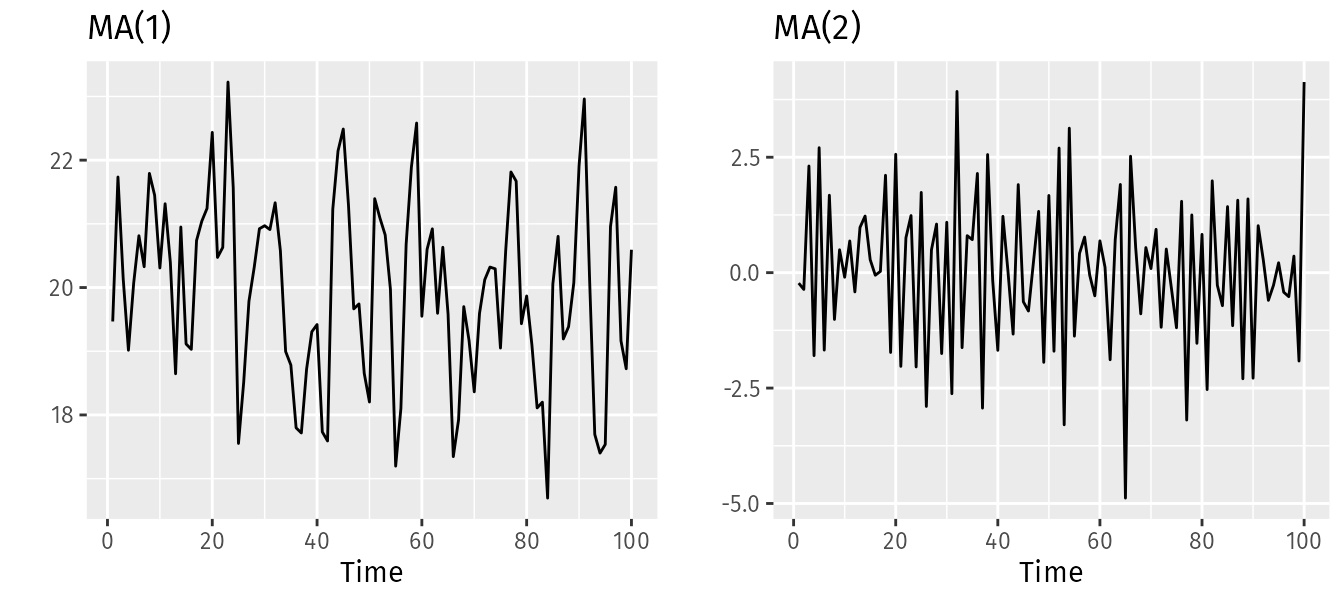
\includegraphics[width=\textwidth]{img/maq-1-example.png}        
        \end{minipage}
    
        \begin{minipage}[t]{0.9\textwidth}
            Fuente: Forecasting: Principles and Practice (Hyndman y Athanasopoulos, 2023). Recuperado de \url{https://otexts.com/fpp2/time-plots.html}
        \end{minipage}
    \end{figure}

    El modelo MA(1) tiene como fórmula: $y_t=20+\varepsilon_t+0.8\varepsilon_t-1$ y el modelo MA(2) tiene como fórmula: $y_t=\varepsilon_t - \varepsilon_t-1 + 0.8\varepsilon_t-2$, en ambos casos $\varepsilon_t$ (ruido blanco) tiene una distribución normal, con promedio igual a 0 y varianza igual a 1 \cite{forecast-time-series-arima}.

    Un modelo AR($p$) estacionario es capaz de ser escrito como un modelo MA($\infty$), esto se puede demostrar para un modelo AR(1)luego de realizar repetidas sustituciones:
    \begin{equation*}
    \begin{split}
    y_t &=\phi_1y_t-1+\varepsilon_t\\  &=\phi_1(\phi_1y_t-2+\varepsilon_t-1)+\varepsilon_t\\ &=\phi^2_1y_t-2+\phi_1\varepsilon_t-1+\varepsilon_t\\ &=\phi^3_1y_t-3+\phi^2_1\varepsilon_t-2+\phi_1\varepsilon_t-1+\varepsilon_t
    \end{split}
    \end{equation*}

    Teniendo $-1>\phi_1<1$, el valor de $\phi^k_1$ irá disminuyendo a medida que $k$ siga creciendo, obteniendo un proceso MA($\infty$) \cite{forecast-time-series-arima}, este tipo de modelo se escribe de la siguiente manera:
    \begin{equation*}
        y_t=\varepsilon_t+\phi_1\varepsilon_t-1+\phi^2_1\varepsilon_t-2+\phi^3_1\varepsilon_t-3+...
    \end{equation*}

    También se puede realizar el proceso inverso, para obtener un modelo AR($\infty$) desde un modelo MA, si es que se definen ciertos limites. Este tipo de modelos que se pueden transcribir de MA a AR($\infty$) y AR a MA($\infty$), son llamados modelos \textbf{invertibles} \cite{forecast-time-series-arima}.
\end{itemize}

Combinando los modelos de diferenciación, autorregresivo y de media móvil obtenemos el modelo \textbf{ARIMA} \cite{forecast-time-series-arima}, este queda modelado de la siguiente manera:
\begin{equation*}
    y'_t=c+\phi_1y'_t-1+...+\phi_py'_t-p+\theta_1\varepsilon_t-1+...+\theta_q\varepsilon_t-q+\varepsilon_t
\end{equation*}

Teniendo en cuenta que $y'_t$ corresponde a la serie diferenciada, a la derecha de la igualdad se encuentran las variables que permiten realizar las predicciones, entre estas se encuentran valores desfasados de $y_t$ y errores desfasados.
El modelo \textbf{ARIMA($p,d,q$)} tiene 3 variables, donde cada una de estas variables esta relacionada a \cite{forecast-time-series-arima}:
\begin{itemize}
    \item $p$ = orden de la parte autorregresiva del modelo.
    \item $d$ = grado de la primera diferenciación.
    \item $q$ = orden de la parte de media móvil.
\end{itemize}

De la misma manera que la estacionariedad e invertibilidad se aplican a los modelos de autorregresión y de media móvil, también se aplican para los modelos ARIMA. Este modelo presenta casos especiales, los cuales representan modelos anteriormente mencionados, los cuales son:
\begin{itemize}
    \item White noise: ARIMA(0,0,0)
    \item Random walk: ARIMA(0,1,0) sin constante
    \item Random walk con desfase: ARIMA(0,1,0) con constante
    \item Autorregresión: ARIMA($p$,0,0)
    \item Media móvil: ARIMA(0,0,$q$)
\end{itemize}

\subsubsection{Modelo SARIMA}
El modelo SARIMA es una extensión del ARIMA, diseñado específicamente para series temporales que presentan estacionalidad. Mientras que ARIMA es eficaz para modelar series no estacionarias sin componentes estacionales, SARIMA incorpora parámetros adicionales para capturar y predecir patrones que se repiten a intervalos regulares en el tiempo.

La estacionalidad en una serie temporal refleja un patrón regular que se repite cada 
\( S \) períodos. Aquí, \( S \) indica el número de períodos requeridos para que el patrón complete un ciclo y comience a repetirse \cite{series-de-tiempo-sarima}.

\begin{itemize}
\item \textbf{Diferenciación no estacional:} Si en los datos se detecta una tendencia, es probable que sea necesario aplicar una diferenciación no estacional. A menudo, al realizar una primera diferenciación no estacional, se logra eliminar la tendencia de la serie temporal. Para este propósito, utilizamos la fórmula:
    \begin{equation*}
        (1 - B) x_t = x_t - x_{t-1}
    \end{equation*}
\end{itemize}

\begin{itemize}
    \item \textbf{Diferenciación para tendencia:} Cuando tanto la tendencia como la estacionalidad están presentes en una serie temporal, es posible que necesitemos aplicar tanto una diferenciación no estacional como una estacional.

    Por lo tanto, es esencial examinar tanto el ACF (Función de Autocorrelación) como el PACF (Función de Autocorrelación Parcial) de la expresión:
    
        \begin{equation*}
            (1 - B^{12})(1 - B) x_t = (x_t - x_{t-1}) - (x_{t-12} - x_{t-13})
        \end{equation*}
    
        Es importante destacar que eliminar la tendencia no necesariamente implica que se haya eliminado toda la dependencia en la serie. Mientras que la tendencia (o el componente de la media) puede haber sido eliminada, aún puede persistir un comportamiento periódico. Al aplicar la diferenciación, descomponemos la dependencia en eventos recientes y eventos a largo plazo \cite{series-de-tiempo-sarima}.    
\end{itemize}

\begin{itemize}
    \item \textbf{Diferenciación para estacionalidad:} Cuando se tienen datos con componentes estacionales, es posible que los componentes no estacionales a corto plazo sigan influyendo en el modelo. Por ejemplo, en el caso de las ventas de componentes electrónicos, las ventas de los últimos uno o dos meses, junto con las ventas del mismo mes del año anterior, pueden ser relevantes para predecir las ventas del mes actual.

    Por lo tanto, es crucial examinar el comportamiento del ACF (Función de Autocorrelación) y PACF (Función de Autocorrelación Parcial) en los primeros rezagos para determinar qué términos no estacionales pueden ser significativos en el modelo.
        
\end{itemize}

Siendo expresado de manera abreviada: 
\begin{equation*}
    (p,d,q) \times (P, D, Q, S)
\end{equation*}

\( P \): Es el número de términos autorregresivos estacionales.

\( D \): Es el grado de diferenciación estacional.

\( Q \): Es el número de términos de promedio móvil estacional.

\( S \): Es el número de periodos en una temporada (por ejemplo, 12 para datos mensuales si se observa una periodicidad anual).



\subsection{Redes LSTM Long Short-Term Memory}
\subsubsection{¿Qué son las redes Long Short-Term Memory?}

La LSTM es un tipo de red neuronal recurrente (RNN) diseñada para resolver el problema del gradiente evanescente mediante la introducción de una célula de memoria que puede almacenar información durante periodos de tiempo más largos \cite{redes-lstm-long-short-term-memory}.

\subsubsection{Arquitectura de una Long Short-Term Memory}

\begin{itemize}
    \item \textbf{Puerta de entrada:} La puerta de entrada en una LSTM utiliza una función de activación sigmoidea para decidir qué valores pasar a la célula de memoria. La función sigmoidea genera valores entre 0 y 1, lo que permite que la puerta de entrada \( decida \) en qué grado un valor debe ser almacenado en la célula de memoria. Un valor cercano a 1 indica que casi toda la información debe ser conservada, mientras que un valor cercano a 0 sugiere que la información debe ser mayormente descartada \cite{redes-lstm-long-short-term-memory}.
\end{itemize}

\begin{itemize}
    \item \textbf{Puerta del Olvido:} Controla qué información de la célula de memoria del paso temporal anterior debe ser conservada y cuál debe ser descartada. Utiliza una función de activación sigmoidea para determinar esto. Un valor cercano a 1 de la sigmoidea indica que la información debe ser conservada, mientras que un valor cercano a 0 indica que debe ser olvidada. \cite{redes-lstm-long-short-term-memory}.
\end{itemize}

\begin{itemize}
    \item \textbf{Puerta de Salida:} Controla qué información de la célula de memoria debe ser enviada como salida. Utiliza una función de activación sigmoidea para decidir qué partes de la memoria se deben considerar y luego aplica una función de tangente hiperbólica para escalar los valores entre -1 y 1, determinando así la salida final de la célula LSTM \cite{redes-lstm-long-short-term-memory}.
\end{itemize}

\begin{itemize}
    \item \textbf{Célula de memoria:} Es el componente central de la arquitectura LSTM. Esta célula almacena información a través del tiempo, pudiendo olvidar selectivamente información no relevante y añadir nueva información a su estado interno.

    En cada paso temporal, el modelo LSTM recibe un vector de entrada junto con un vector de estado oculto proveniente del paso temporal anterior. A partir de estos, la puerta de entrada decide qué nueva información se debe almacenar en la célula de memoria, mientras que la puerta de olvido decide qué información previamente almacenada debe descartarse.
    
    Después, se genera un estado candidato utilizando la función de activación tangente hiperbólica. Este estado candidato se combina con el estado actual de la célula de memoria mediante una operación de suma elemento a elemento, actualizando así la información almacenada.
    
    Finalmente, la puerta de salida determina cuál de esta información actualizada se emitirá como salida de la LSTM. Este output, junto con el estado actualizado de la célula de memoria, se pasa al siguiente paso temporal \cite{redes-lstm-long-short-term-memory}.
    
\end{itemize}



\subsection{Metodología del proyecto}
Para llevar a cabo el desarrollo del proyecto, se definieron cuatro fases que corresponden a la totalidad del proyecto, las cuales corresponden a:

\subsubsection{Fase 1: Planteamiento y planificación}

Para la primera fase del proyecto, se llevará a cabo una planificación de la manera en la que será abordada la problemática, para desarrollar un anteproyecto que será utilizado para evaluar y planificar las actividades correspondientes al desarrollo del proyecto. Entre ellas se encuentran:

\begin{itemize}
    \item Planteamiento del proyecto y sus objetivos.
    \item Definición de alcances y limitaciones.
    \item Creación de un cronograma de actividades.
\end{itemize}

\subsubsection{Fase 2: Investigación}

Para la segunda fase, se realizará una investigación de herramientas y recursos necesarios para llevar a cabo un diseño de la solución para la problemática del proyecto planteado, sumado a un análisis de las bases de datos brindadas por la empresa AFP Capital. Una vez realizado lo anterior, se llevará a cabo una propuesta de diseño para la problemática, siendo entregada y analizada por la empresa, con la finalidad de pasar a desarrollo. Algunas de las actividades de esta fase corresponden a:

\begin{itemize}
    \item Investigación del problema.
    \item Toma de requerimientos.
    \item Investigación de tecnologías de análisis de datos.
\end{itemize}

\subsubsection{Fase 3: Modelamiento y desarrollo}
Para la tercera fase, se llevará a cabo el diseño y desarrollo del sistema propuesto, además de realizar pruebas para verificar el correcto funcionamiento. Algunas de las actividades de esta fase corresponden a:

\begin{itemize}
    \item Modelado del sistema ETL.
    \item Modelado de la API.
    \item Implementación del modelo propuesto.
    \item Pruebas y validaciones.
    \item Correcciones de errores.
\end{itemize}

\subsubsection{Fase 4: Conclusiones y recomendaciones}
Para la última fase, se dará fin al desarrollo del proyecto, elaborando un manual de usuario el cual indicaría algunas funcionalidades del sistema. Algunas de las actividades de esta fase corresponden a:

\begin{itemize}
    \item Desarrollo de manual de usuario.
    \item Redacción de conclusiones y recomendaciones.
    \item Cierre del proyecto.
\end{itemize}


\subsection{Metodología del sistema}
\subsubsection{CRISP-DM}
La metodología CRISP-DM (Cross-Industry Standard Process for Data Mining) es un proceso estándar utilizado para realizar proyectos de minería de datos. La metodología CRISP-DM se divide en seis fases distintas que se describen a continuación:

\begin{enumerate}
    \item \textbf{Comprensión del problema:} En esta fase se define el problema a resolver y se establecen los objetivos del proyecto. También se recopilan los datos necesarios para el proyecto.
    \item \textbf{Comprensión de los datos:} En esta fase se realiza una exploración de los datos para comprender su calidad, estructura y relevancia para el problema en cuestión.
    \item \textbf{Preparación de los datos:} En esta fase se limpian y procesan los datos para que puedan ser utilizados en la etapa de modelado.
    \item \textbf{Modelado:} En esta fase se aplican técnicas de modelado para desarrollar un modelo predictivo. Se prueban diferentes modelos y se selecciona el que mejor se ajuste a los datos.
    \item \textbf{Evaluación:} En esta fase se evalúa el modelo desarrollado en la fase anterior. Se verifica que el modelo funcione correctamente y se ajuste adecuadamente a los datos.
    \item \textbf{Implementación:} En esta fase se implementa el modelo desarrollado en la fase de modelado en un entorno de producción. También se establecen planes para monitorear el rendimiento del modelo y actualizarlo según sea necesario.
\end{enumerate}

Las fases de la metodología CRISP-DM son iterativas, lo que significa que es posible volver a una fase anterior si es necesario.

\subsubsection{OSEMN}

La metodología OSEMN (acrónimo de las palabras en inglés: Obtain, Scrub, Explore, Model, Interpret) es un proceso utilizado en la minería de datos y el análisis de datos para trabajar con grandes conjuntos de datos de manera efectiva. 

\begin{enumerate}
    \item \textbf{Obtener (Obtain):} En esta etapa, se recopilan los datos necesarios para el análisis. Los datos pueden provenir de diferentes fuentes, como bases de datos, archivos en línea o registros de sensores. La calidad y la cantidad de los datos obtenidos son cruciales para el éxito del análisis.
    \item \textbf{Limpieza (Scrub):} Una vez que se han obtenido los datos, es necesario realizar una limpieza para eliminar datos innecesarios o incorrectos. Esta etapa puede implicar la eliminación de duplicados, la corrección de errores y la eliminación de valores atípicos. El objetivo de esta etapa es obtener datos limpios y coherentes para el análisis.
    \item \textbf{Exploración (Explore):} En esta etapa, se utilizan técnicas de visualización y estadísticas para explorar los datos y obtener información sobre ellos. Se pueden identificar patrones, tendencias y relaciones entre diferentes variables. El objetivo es obtener una comprensión más profunda de los datos y de cómo se relacionan entre sí.
    \item \textbf{Modelado (Model):} En esta etapa, se utilizan técnicas de modelado estadístico o de aprendizaje automático para crear modelos que puedan predecir resultados futuros o identificar patrones en los datos. El objetivo es utilizar los datos para crear un modelo que pueda utilizarse para tomar decisiones informadas.
    \item \textbf{Interpretación (Interpret):} En esta etapa, se interpretan los resultados obtenidos en la etapa de modelado. Los resultados pueden ser utilizados para tomar decisiones o para generar nuevas hipótesis que puedan ser exploradas en futuros análisis.
\end{enumerate}

Se propone el uso de la metodología OSEMN, ya que se enfoca en el análisis de datos y la creación de modelos predictivos. OSEMN también es una metodología más flexible que CRISP-DM, lo que puede ser útil en un proyecto de SCRUM donde se busca una mayor adaptabilidad.

Por otro lado, también se propone el uso de la metodología CRISP-DM, ya que el proyecto incluye una etapa de exploración y análisis de datos, seguida por una fase de construcción de modelos. CRISP-DM se enfoca en el proceso completo de minería de datos, desde la comprensión del problema hasta la implementación del modelo, lo que puede servir para realizar un trabajo más estructurado.

Ya que este proyecto se encuentra bajo el marco de trabajo SCRUM, ambas metodologías pueden ser utilizadas de manera complementaria, utilizando OSEMN para las fases de creación de modelos y CRISP-DM para la etapa de exploración y análisis de datos.


\chapter{Proceso ETL}

El proceso ETL (Extract, Transform, Load) representa el núcleo de la gestión de datos en numerosas organizaciones, desempeñando un papel esencial en la recopilación, transformación y carga de información crítica. En este capítulo del informe, exploraremos en detalle el funcionamiento de un proceso ETL, así como su diseño estratégico. Analizaremos cómo esta metodología se convierte en una piedra angular para la toma de decisiones basadas en datos y la mejora de la eficiencia operativa.
\section{Diseño Proceso ETL}
\input{Proceso ETL/Diseño Proceso ETL.tex}

\subsection{Requisitos ETL}
En esta etapa se definen los requisitos del proyecto, las fuentes de datos, los objetivos comerciales y del proceso ETL, las necesidades de análisis y los plazos para realizar el proceso. Estableciendo una base solida para el diseño y buen funcionamiento del proceso ETL.
\begin{itemize}
    \item Fuente de datos: La fuente de datos corresponde a un archivo .CSV que contiene información de la navegación web de los clientes en forma de Web Logs.
    \item Objetivos comerciales: Analizar el comportamiento de los clientes y sus preferencias de uso en un período igual o inferior a 6 meses, para poder predecir navegaciones futuras personalizadas
    \item Objetivos proceso ETL: Realizar las transformaciones necesarias para asegurar que el flujo de datos sea eficiente y preciso, a través de la limpieza de los daotsm normalización, agregación, filtrado, enriquecimiento de datos, cálculos y derivaciones necesarias.
    \item Necesidades de análisis: Realizar un análisis exploratorio de los datos entregados.
\end{itemize}


\subsection{Identificicación fuente de datos}
En esta etapa se determinan las fuentes de datos a ser usadas para el proyecto, incluyendo bases de datos y archivos .CSV y API´s. Esto además comprende la estructura la definición de la estructura, el formato y ubicación de cada fuente de datos dentro del proyecto.


\subsection{Diseño del modelo de datos objetivo}
En esta etapa, se lleva a cabo el diseño del modelo de datos objetivo. Dado el tipo de proyecto, no será necesario crear un modelo multidimensional u algo similar para su implementación. Esto se debe a que los datos de entrada para los algoritmos predictivos consistirán en datos planos, en forma de Dataframes de pandas.

\subsection{Planificación de las transformaciones}
Dentro de esta etapa se realiza la planificación detallada de las transformaciones necesarias para construir una base sólida y consistente para el desarrollo del proyecto. Estas transformaciones implican una serie de pasos que permiten limpiar, filtrar, combinar y enriquecer los datos de manera adecuada.

La planificación de las transformaciones es fundamental para garantizar la calidad y la integridad de los datos que serán utilizados en el proyecto. Durante esta etapa, se identifican las tareas específicas que deben llevarse a cabo para lograr los objetivos establecidos, teniendo en cuenta los requisitos del proyecto y las necesidades del negocio.

Algunas de las transformaciones comunes incluyen \cite{etl-toolkit}:

\begin{itemize}
    \item \textbf{Limpieza de datos:} Se realizan tareas de limpieza para corregir errores, eliminar valores duplicados o inconsistentes, y garantizar la coherencia de los datos. Esto puede incluir la corrección de formatos incorrectos, la normalización de datos, el manejo de valores faltantes o la estandarización de la información. La limpieza se realizo para solo tomar el cuenta los valores no nulos y se establecío el formato 'YYYY;MM;DD;HH;MM;SS.ss' de la columna 'fecha evento'.

    \item \textbf{Filtrado de datos:} Se aplican filtros para seleccionar y extraer los datos relevantes para el proyecto, descartando aquellos que no cumplen con ciertos criterios o condiciones específicas, \textbf{no permitiendo registros sin métodos asociados}. Esto ayuda a reducir el volumen de datos y a enfocarse en la información más relevante y útil.

    \item \textbf{Combinación de datos:} Se integran datos provenientes de diferentes fuentes o fuentes de datos diversas. Esto implica fusionar conjuntos de datos relacionados, realizar uniones o cruces de tablas, y establecer relaciones entre los datos para generar una visión global y coherente.

    \item \textbf{Enriquecimiento de datos:} Se agregan atributos o información adicional a los datos existentes para enriquecer su contexto y mejorar su valor. Esto puede implicar la incorporación de datos externos, la realización de cálculos derivados, la normalización de datos o la aplicación de reglas específicas.
\end{itemize}


Es importante tener en cuenta que la planificación de las transformaciones considera el orden y la secuencia adecuada de ejecución, así como la documentación de cada paso y los criterios de validación y verificación para garantizar la calidad de los datos transformados.
% Por esto es que se diseño el siguiente plan detallado con las transformaciones a aplicar.


\subsection{Selección de herramientas}
En esta etapa, se realiza la selección de herramientas de software que se ajusten a las necesidades y requisitos del proyecto para llevar a cabo el proceso ETL de manera eficiente. Se evalúan diferentes opciones disponibles en función de su capacidad, compatibilidad y facilidad de uso, para garantizar una elección adecuada, es por esto que se seleccionaron las siguientes herramientas:
\begin{itemize}
    \item \textbf{Colab}: También conocido como "Colaboratory", permite programar y ejecutar Python en el navegador con las siguientes ventajas \cite{colab}:
    \begin{itemize}
        \item No requiere configuración
        \item Acceso a GPUs sin coste adicional
        \item Permite compartir contenido fácilmente
    \end{itemize}
    Una de las desventajas de usar Colab es que tiene una cantidad de memoria limitada, es decir, si se utiliza el total de memoria disponible no se podrá seguir ejecutando código.
    \item \textbf{Visual Studio Code:} Es un editor de código fuente desarrollado por Microsoft. Es conocido por su enfoque en la simplicidad, la personalización y la eficiencia. Este editor se utilizará en caso de no poder seguir utilizando Colab.
    \item \textbf{Python:} Es un lenguaje de programación interpretado, de alto nivel y de propósito general, conocido por su sintaxis clara y legible. Es utilizado en una amplia gama de aplicaciones, desde desarrollo web hasta ciencia de datos y aprendizaje automático. Python se destaca por su facilidad de aprendizaje y su amplia biblioteca estándar, que ofrece numerosas funcionalidades predefinidas para diversas tareas \cite{python}.
    \begin{itemize}
        \item \textbf{Numpy:} Es una biblioteca fundamental para la computación científica en Python. Proporciona estructuras de datos eficientes y funciones para realizar operaciones numéricas y de manipulación de arrays \cite{numpy}.
        \item \textbf{Pandas:} Es una biblioteca poderosa para el análisis de datos basada en Numpy, que proporciona estructuras de datos flexibles y eficientes, como DataFrames, y un conjunto completo de funciones para la manipulación y transformación de datos \cite{pandas}.
        \item \textbf{Dask:} Es una biblioteca de paralelización flexible que permite escalar el procesamiento de datos en Python. Proporciona estructuras de datos paralelas y operaciones distribuidas que facilitan el procesamiento de grandes volúmenes de datos \cite{dask}.
    \end{itemize}
\end{itemize}


\subsection{Construcción y prueba proceso ETL}
En esta etapa, se lleva a cabo la implementación del diseño del proceso ETL previamente definido, utilizando las herramientas seleccionadas. Se desarrollan los flujos de extracción, transformación y carga de los datos según lo establecido en el diseño.

Una vez implementado, se procede a realizar pruebas exhaustivas para garantizar el correcto funcionamiento del proceso. Estas pruebas incluyen la verificación de la extracción de datos de las fuentes, la correcta aplicación de las transformaciones definidas y la carga exitosa de los datos en el destino final.

El objetivo de las pruebas es asegurar que el proceso ETL cumpla con los requisitos establecidos y que los resultados obtenidos sean los esperados. Esto implica validar la integridad y coherencia de los datos transformados, así como verificar el rendimiento y la escalabilidad del proceso.

En caso de encontrar inconvenientes o desviaciones durante las pruebas, se realizan los ajustes necesarios en el diseño o en la configuración de las herramientas utilizadas. Es fundamental realizar iteraciones y pruebas adicionales hasta obtener resultados consistentes y satisfactorios.

Como primer paso en la construcción del proceso ETL, se importan las bibliotecas pandas y numpy. Luego se le da nombre a las columnas, ya que el contenido del archivo csv solo trae los datos. Una vez nombradas las columnas se ordenan para un entendimiento más facil del conjunto de datos, quedando de la siguiente manera respectivamente: rut, fecha, metodo, canal.

Ahora se comprueba la existencia de valores nulos en el dataframe, resultando lo siguiente:

\begin{figure}[H]
    \begin{minipage}[t]{0.8\textwidth}
        \caption{Valores nulos en el conjunto de datos.}
        \label{valoresNulos}        
    \end{minipage}

    \vspace{10pt}

    \centering
    \begin{minipage}[b]{0.4\textwidth}
        \centering
        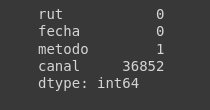
\includegraphics[width=\textwidth]{img/valores-nulos.png}        
    \end{minipage}

    \begin{minipage}[t]{0.9\textwidth}
        Fuente: Elaboración propia.
    \end{minipage}
\end{figure}

Como se puede ver en la imagen anterior solamente los campos 'metodo' y 'canal' poseen valores nulos, de hecho, el primero solo cuenta con un valor nulo. La columna 'canal' cuenta con 36852 valores nulos. Luego de eliminar los valores nulos se pasa a eliminar las filas que contengan métodos inconsistentes, que son:
\begin{itemize}
    \item clientes/surveys
    \item clientes/cuentas/validar-cuenta-corriente
    \item clientes/cuentas/cuentas-bancarias
    \item clientes/cuentas/cuentas-bancarias?rut=81550425
    \item clientes/cuentas/cuentas-bancarias?rut=81691037
    \item clientes/cuentas/cuentas-bancarias?rut=243990041
    \item clientes/cuentas/cuentas-bancarias?rut=12501979K
    \item clientes/cuentas/cuentas-bancarias?rut=169262780
    \item clientes/cuentas/cuentas-bancarias?rut=55022526
    \item clientes/cuentas/cuentas-bancarias?rut=134382953
    \item clientes/cuentas/cuentas-bancarias?rut=126599692
    \item clientes/cuentas/APV/solicitud/giros?rut=151980287\&account=APV
    \item clientes/cuentas/cuentas-bancarias?rut=172165532
\end{itemize}

Al eliminar todas las filas que contengan los métodos antes mencionados se borran un total de 1447 registros. Finalmente, se eliman un total de 38299 filas del dataset original.

\subsection{Monitoreo proceso ETL}
Se establece un sistema de monitoreo para poder supervisar el rendimiento del proceso ETL, logrando identificar posibles problemas y garantizar la calidad de los datos. Es en esta etapa donde se hace un mantenimiento del proceso, pudiendo tener actualizaciones de las transformaciones, resolución de problemas y optimizar el proceso.

\chapter{\nohyphens{Exploratory Data Analysis (EDA)}}

El análisis exploratorio de datos (EDA) es una etapa crucial en el proyecto de predicción del comportamiento en un entorno web. En este capítulo, adentraremos en el proceso de EDA, que nos permitirá desvelar patrones, tendencias y relaciones ocultas en los datos recopilados. A través de este análisis, obtendremos una visión profunda y enriquecedora que sentará las bases para un mejor entendimiento del comportamiento del usuario en el entorno web y facilitará la toma de decisiones estratégicas.

\section{Introducción al EDA}
%Breve descripción del objetivo del análisis exploratorio de datos.
%Explicación de la importancia de comprender los datos antes de construir el modelo de predicción de comportamiento de los clientes.
El análisis exploratorio de datos (EDA, por sus siglas en inglés, Exploratory Data Analysis) es una fase fundamental en la investigación y comprensión de un conjunto de datos. Como su nombre lo indica, el EDA tiene como objetivo explorar y examinar los datos de manera detallada, utilizando resúmenes numéricos y visuales, con el fin de descubrir patrones, tendencias y características no anticipadas. Es considerado uno de los primeros pasos en el proceso de análisis, ya que proporciona una visión general de los datos antes de realizar un análisis más profundo \cite{ruiz2022exploratorio}.

El enfoque principal del EDA radica en el uso de herramientas y técnicas visuales y gráficas para revelar información clave sobre los datos en estudio \cite{parra2002exploratorio}. Estas técnicas incluyen el diagrama de tallo y hoja, el diagrama de caja y bigotes, y el diagrama de dispersión, entre otros. Al aplicar estas técnicas de análisis gráfico, podemos obtener una comprensión más profunda de la distribución y estructura de los datos, así como identificar relaciones entre las variables de interés. Además, el EDA nos brinda la capacidad de detectar posibles errores o puntos extremos, como anomalías, que podrían afectar la calidad de los resultados del análisis.

Los beneficios clave del análisis exploratorio de datos son los siguientes:
\begin{itemize}
    \item \textbf{Conocer la distribución y estructura de los datos:} El EDA nos permite examinar la distribución de las variables y comprender cómo se organizan y dispersan los datos en el conjunto. Esto es fundamental para seleccionar las técnicas adecuadas de análisis estadístico y modelado.
    \item \textbf{Estudiar la relación entre variables:} Mediante el análisis de correlación y la visualización de patrones en los diagramas de dispersión, podemos explorar las relaciones entre las variables y comprender cómo interactúan entre sí. Esto nos brinda información valiosa para identificar posibles dependencias y tendencias en los datos.
    \item \textbf{Encontrar posibles errores y anomalías:} El EDA nos ayuda a identificar valores atípicos, datos faltantes u otros errores en los datos. Estas anomalías pueden tener un impacto significativo en los resultados del análisis, por lo que es importante detectarlas y tratarlas de manera adecuada.
\end{itemize}

\section{Recopilación de datos}
Los datos recopilados de los registros de navegación de los afiliados de AFP Capital constituyen una valiosa fuente de información para comprender el comportamiento y las preferencias de los usuarios en la plataforma web. Estos registros nos permiten analizar cómo interactúan los afiliados con los diferentes canales y métodos disponibles, así como realizar un seguimiento detallado de las fechas y horarios en que se llevan a cabo estas interacciones.

El dataset inicial entregado para este proyecto cuenta con 58,252 registros de navegación de usuarios, lo cual proporciona una cantidad significativa de información para su análisis. Antes de utilizar estos datos, se realizó un proceso de anonimización para proteger la privacidad de los usuarios, específicamente modificando el campo del rut para no mostrar el dato original. De esta manera, se garantiza que los registros sean tratados de forma confidencial y segura.

Los cuatro campos principales que conforman el conjunto de datos son el rut, la fecha del evento, el método y el canal. El rut, que ha sido modificado, actúa como un identificador único para cada usuario y permite realizar análisis individuales sin revelar su identidad. La fecha del evento registra el momento exacto en que se llevó a cabo cada navegación, lo cual es crucial para identificar patrones y tendencias a lo largo del tiempo. El campo del método describe la interacción específica realizada por el usuario en el canal correspondiente, proporcionando información detallada sobre las acciones que realizan. Por último, el campo del canal indica el sitio o ambiente particular en el cual tuvo lugar cada interacción, lo que puede ser útil para comprender las preferencias de los usuarios en relación con los diferentes entornos disponibles.

Con respecto al preprocesamiento de datos realizado hasta la fecha, se ha seguido el proceso ETL (Extracción, Transformación y Carga) que se describe en detalle en el capítulo anterior. Este proceso implica extraer los datos de las fuentes de origen, transformarlos en un formato adecuado y cargarlos en un sistema de almacenamiento para su posterior análisis. Se utilizaron diversas herramientas especializadas para llevar a cabo estas tareas, asegurando la calidad y coherencia de los datos procesados.

Es importante destacar que, si bien los datos recopilados ofrecen una valiosa perspectiva sobre el comportamiento de los usuarios en la plataforma web, es necesario tener en cuenta que existe un sesgo en la muestra de datos. En particular, los registros de navegación corresponden principalmente a afiliados con rentas altas. Esto implica que los usuarios con ingresos más altos, aquellos que cotizan por un valor elevado o el valor máximo, están sobrerrepresentados en la muestra. Por lo tanto, al interpretar y generalizar los resultados obtenidos, es fundamental tener en cuenta esta limitación y considerar posibles variaciones en el comportamiento de otros segmentos de usuarios.

\section{Descripción de los datos}
Resumen de las principales estadísticas descriptivas de las variables relevantes en los logs de navegación.
Análisis de la distribución de los datos, incluyendo medidas de centralidad y dispersión.
Haciendo uso de la librería pandas podemos obtener informacion respecto al dataframe, cantidad de valores únicos y calcular estadísticas descriptivas:

Podemos obtener informacion respecto a la cantidad de valores faltantes de cada dataframe que se está utilizando, los cuales son \textbf{36853}:

\begin{figure}[H]
    \begin{minipage}[t]{0.9\textwidth}
        \caption{Datos faltantes dataframes.}
        \label{descripcion_dataframe}        
    \end{minipage}

    \vspace{10pt}

    \begin{minipage}[b]{0.85\textwidth}
        \centering
        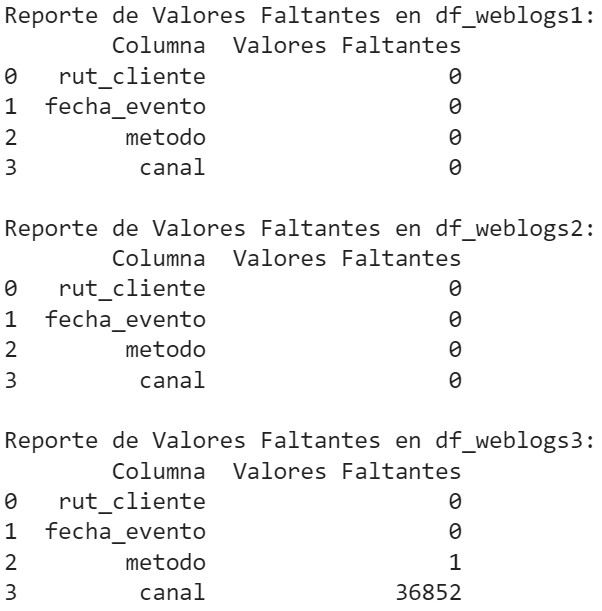
\includegraphics[width=\textwidth]{img/valores faltantes datasets.jpg}        
    \end{minipage}

    \begin{minipage}[t]{0.9\textwidth}
        Fuente: Elaboración propia.
    \end{minipage}
\end{figure}

\begin{itemize}
    \item \textbf{rut cliente:} Contiene datos de tipo int64.
    \item \textbf{fecha evento:} Contiene datos de tipo object.
    \item \textbf{metodo:} Contiene datos de tipo object.
    \item \textbf{canal:} Contiene datos de tipo object.
\end{itemize}

Además se puede conocer la cantidad de valores únicos que posee cada una de las columnas de los 2 datasets:

Dataset 1:

\begin{itemize}
    \item \textbf{rut cliente:} Contiene 40125 valores únicos.
    \item \textbf{fecha evento:} Contiene 80181 valores únicos.
    \item \textbf{metodo:} Contiene 81254 valores únicos.
    \item \textbf{canal:} Contiene 81254 valores únicos.
\end{itemize}

Dataset 2:

\begin{itemize}
    \item \textbf{rut cliente:} Contiene 40224 valores únicos.
    \item \textbf{fecha evento:} Contiene 80470 valores únicos.
    \item \textbf{metodo:} Contiene 81546 valores únicos.
    \item \textbf{canal:} Contiene 81546 valores únicos.
\end{itemize}

La librería pandas ofrece una buena cantidad de estadísticas descriptivas gracias a su función .describe, las cuales se muestran a continuación:
\begin{itemize}
    \item \textbf{Recuento (count):} Calcula el número de valores no nulos en cada columna. \textbf{count: 58009.000000} valores no nulos.
    \item \textbf{Media (mean):} Calcula la media de las columnas numéricas. \textbf{mean: 504.854902} 
    \item \textbf{Desviación estándar (std):} Calcula la desviación estándar de las columnas numéricas. \textbf{std: 553.964179}
    \item \textbf{Mínimo (min):} Calcula el valor mínimo de las columnas numéricas. \textbf{min: 1.000000}
    \item \textbf{Cuartiles:} Calcula los cuartiles de las columnas numéricas 
    \begin{itemize}
        \item \textbf{25\%: 8.000000}
        \item \textbf{50\%: 303.000000}
        \item \textbf{75\%: 884.000000}
    \end{itemize}
    \item \textbf{Máximo (max):} Calcula el valor máximo de las columnas numéricas. \textbf{max: 1815.000000}
\end{itemize}
%Identificación de cualquier valor atípico o dato faltante en los registros y discusión sobre cómo se manejarán estos casos.

% \subsection{Visualizaión de datos}
% Utilización de gráficos y visualizaciones para explorar los datos.
Representación visual de las características relevantes de los clientes y su comportamiento en el canal web.



%Análisis de patrones, tendencias o relaciones identificadas a través de las visualizaciones.

%\subsection{Análisis de correlación}
%%Exploración de la relación entre las variables relevantes en los logs de navegación.
%Cálculo de coeficientes de correlación u otras medidas para evaluar la fuerza y dirección de las relaciones.
%Interpretación de los resultados obtenidos y discusión sobre cómo pueden influir en el modelo de predicción.

%\subsection{Análisis de variables importantes}
%%Identificación de las variables más relevantes o influyentes en el comportamiento de los clientes.
%Uso de técnicas estadísticas o algoritmos de selección de características para determinar la importancia relativa de las variables.
%Discusión de los hallazgos y cómo se utilizarán en el modelo de predicción.

%\subsection{Resultados}
%%Resumen de los principales hallazgos del análisis exploratorio de datos.
%Discusión de las implicaciones de estos hallazgos en el proyecto de %empresa y el modelo de predicción de comportamiento de los clientes.
%Posibles limitaciones del análisis exploratorio y propuestas de futuras investigaciones.

\chapter[Modelos de predicción aplicados]{Modelos de\\ predicción aplicados}

\section{Modelo de series de tiempo}
Se implementó un modelo de series de tiempo ARIMA o modelo autorregresivo de media móvil integrado, un modelo centrado en describir las autocorrelaciones que existen entre los datos e intentar predecir y comprender el comportamiento del usuario.

\subsection{Preprocesamiento y Preparación de Datos}

Comenzamos con la carga de los datos desde un archivo CSV, seguida de un proceso de limpieza para asegurar la integridad de la información. En esta etapa, se filtraron registros específicos en la columna “metodo” y se descartaron aquellos casos donde la columna “canal” estaba vacía. Adicionalmente, la columna "fecha\_evento" fue convertida al formato UTC para poder garantizar una estandarización completa a lo largo del conjunto de datos.

\subsection{Codificación y Transformación One-Hot}

Se transformaron las variables categóricas 'método' y 'canal' en representaciones numéricas que son adecuadas para el procesamiento del modelo.

\begin{itemize}
    \item \textbf{Normalización de Fechas:} La columna 'fecha\_evento', que contenía información de fecha y hora, se dividió y estandarizó para asegurar un formato uniforme y utilizable.
    \item \textbf{Eliminación de columnas innecesarias:} Las columnas originales de 'método' y 'canal' se eliminaron después de la codificación, manteniendo el dataset conciso y enfocado en las características relevantes.
    \item \textbf{Transformación Temporal Adicional:} Se llevaron a cabo codificaciones one-hot para las columnas de 'fecha', 'hora' y 'día del mes', ampliando la representatividad de los aspectos temporales de los datos.
    \item \textbf{Transformación y normalización de columna 'metodo':} Se llevo a cabo una transformación de la columna 'metodo' para tener valores numéricos de 0 a $n-1$ y luego se normalizaron estos valores para obtener datos entre 0 y 1. 
\end{itemize}

\subsection{Construcción y Entrenamiento del Modelo}

El dataset fue sometido al test estadístico Dicker-Fuller Aumentada (ADF) para saber si corresponde a una serie de tiempo estacionaria o no, la variable que nos dira si la serie de tiempo es estacionaria o no, es $P\_value$, si $p<0.05$ quiere decir que la serie de tiempo es estacionaria, en el caso de que $p>0.05$ quiere decir que la serie de tiempo no es estacionaria.
Luego, debido a incidencias que se mencionaran más adelante, se decide aplicar el modelo ARIMA sobre un cliente, con el fin de probar el funcionamiento del modelo a la hora de predecir el comporatmiento de un cliente. Ocupando el modulo 'auto\_arima' buscamos un modelo ARIMA$(p,d,q)$ más optimo, el que minimice el valor AIC (Akaike information criterion). 
El dataset es dividido en conjuntos de entrenamiento y validación, luego se implementó el modelo en el set de datos de entrenamiento y el orden $(p,d,q)$ obtenido anteriormente con el modulo 'auto\_arima'.

\subsection{Conclusión del Modelo de series de tiempo ARIMA}

Debido a la naturaleza de los datos, el modelo ARIMA no puede entregar resultados significativos, esto gracias a que la variable objetivo 'metodo' contiene eventos categóricos y el modelo ARIMA esta pensado para predecir numéricos en series de tiempo. También, para poder predecir el comportamiento de cada cliente se tendría que implementar un modelo ARIMA por cliente, haciendo el proceso a gran escala lento y poco eficaz.


\section{Modelo de autoencoders}
Se implementó un modelo de autoencoder como parte de una estrategia de aprendizaje no supervisado para predecir y entender el comportamiento del usuario a partir de un conjunto de datos complejo.

\subsection{Preprocesamiento y Preparación de Datos}

Iniciamos con la carga del dataset desde un archivo CSV, seguido por una fase de limpieza de datos para garantizar la calidad del entrenamiento. Se realizaron las siguientes operaciones de preprocesamiento en los datos.

\subsection{Codificación One-Hot}

Para las variables categóricas \textquotedblleft método\textquotedblright y \textquotedblleft canal\textquotedblright, se aplicó una técnica de codificación One-Hot. Esta transformación es crucial para convertir datos categóricos en un formato que pueda ser procesado efectivamente por el modelo de aprendizaje automático. En esta técnica, cada categoría se convierte en una nueva columna, donde la presencia de una categoría específica se marca con un \textquotedblleft 1\textquotedblright, mientras que las demás se marcan con un \textquotedblleft 0\textquotedblright.

\begin{itemize}
    \item \textbf{Normalización de Fechas:} La columna \textquotedblleft fecha\_evento\textquotedblright, que contenía información de fecha y hora, se dividió y estandarizó para asegurar un formato uniforme y utilizable.
    \item \textbf{Eliminación de columnas innecesarias:} Las columnas originales de \textquotedblleft método\textquotedblright y \textquotedblleft canal\textquotedblright se eliminaron después de la codificación, manteniendo el dataset conciso y enfocado en las características relevantes.
    \item \textbf{Transformación Temporal Adicional:} Se llevaron a cabo codificaciones one-hot para las columnas de \textquotedblleft fecha\textquotedblright, \textquotedblleft hora\textquotedblright y \textquotedblleft día de la semana\textquotedblright, ampliando la representatividad de los aspectos temporales de los datos.
\end{itemize}

\begin{figure}[H]
    \begin{minipage}[t]{0.9\textwidth}
        \caption{Preparación y codificación one-hot de los datos}
        \label{codificación_autoencoder}        
    \end{minipage}

    \vspace{10pt}

    \begin{minipage}[b]{0.9\textwidth}
        \centering
        \includegraphics[width=\textwidth]{img/codificación one-hhot.jpg}        
    \end{minipage}

    \begin{minipage}[t]{0.9\textwidth}
        Fuente: Elaboración propia.
    \end{minipage}
\end{figure}


\subsection{Construcción y Entrenamiento del Modelo}

El dataset fue dividido en conjuntos de entrenamiento y validación. Luego, se construyó la arquitectura del autoencoder con capas densas y normalización por lotes, utilizando una función de activación \textquotedblleft tanh\textquotedblright para las capas codificadoras y \textquotedblleft relu\textquotedblright para las decodificadoras. Se implementó un mecanismo de EarlyStopping para prevenir el sobreentrenamiento y mejorar la generalización del modelo.

Un autoencoder es un tipo de red neuronal utilizada en el aprendizaje no supervisado, que tiene como objetivo aprender una representación (codificación) de un conjunto de datos, típicamente para reducción de dimensionalidad, aprendizaje de características, o descompresión de datos. La particularidad de los autoencoders reside en que están diseñados para reconstruir su entrada en la salida, pasando la información a través de una serie de capas que primero comprimen los datos (codificador) y luego los reconstruyen (decodificador).

En el caso de un autoencoder con \textquotedblleft capas densas" (también conocidas como \textquotedblleft capas completamente conectadas"), cada neurona en una capa está conectada a todas las neuronas en la capa siguiente. Este tipo de arquitectura es una de las más comunes en las redes neuronales y es particularmente útil para aprender patrones complejos y no lineales en los datos.

\textbf{Construcción del Codificador:} En la parte del codificador, los datos de entrada pasan a través de capas densas, donde se reduce gradualmente la dimensionalidad. Este proceso se logra reduciendo el número de neuronas en capas sucesivas, obligando así a la red a aprender una representación comprimida de los datos de entrada. Las funciones de activación como \textquotedblleft tanh" (tangente hiperbólica) pueden ser usadas aquí para introducir no linealidades en el modelo, permitiendo que el codificador aprenda representaciones más complejas.

\textbf{Construcción del Decodificador:} La segunda parte del autoencoder es el decodificador, donde la representación comprimida se procesa a través de otras capas densas para reconstruir los datos de entrada. El objetivo es que la salida sea lo más cercana posible a la entrada original. Las funciones de activación como \textquotedblleft relu" (Rectified Linear Unit) son comunes en esta etapa, proporcionando una manera eficiente y efectiva de realizar operaciones no lineales.

\begin{figure}[H]
    \begin{minipage}[t]{0.9\textwidth}
        \caption{Arquitectura del modelo autoencoder}
        \label{arquitectura_autoencoder}        
    \end{minipage}

    \vspace{10pt}

    \begin{minipage}[b]{0.99\textwidth}
        \centering
        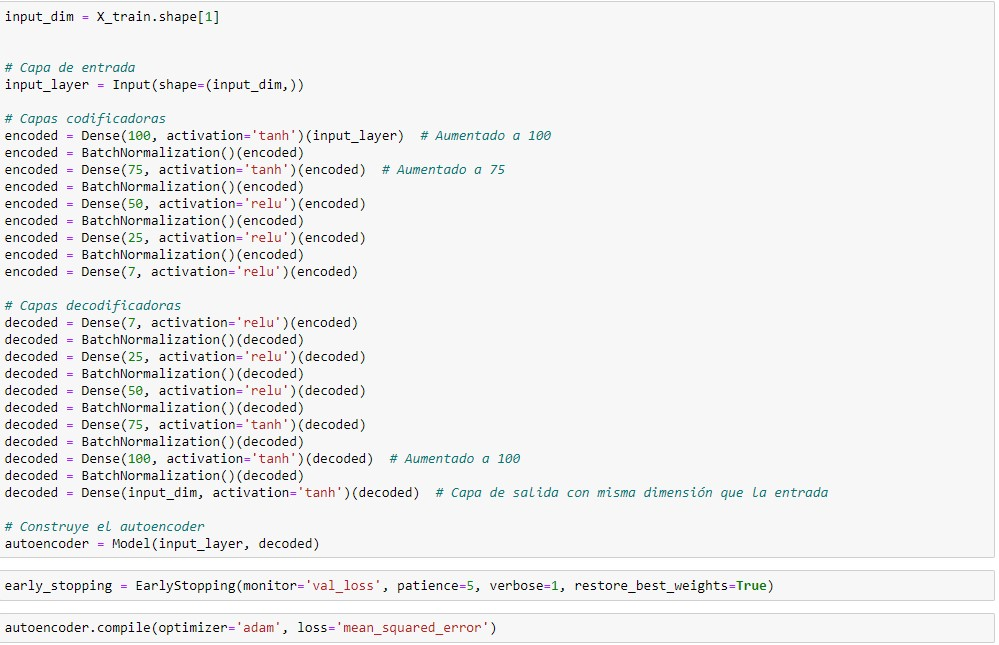
\includegraphics[width=\textwidth]{img/Arquitectura modelo autoencoder.jpg}        
    \end{minipage}

    \begin{minipage}[t]{0.9\textwidth}
        Fuente: Elaboración propia.
    \end{minipage}
\end{figure}

El entrenamiento del autoencoder se realizó adoptando un enfoque iterativo y dinámico, donde uno de los aspectos clave fue el monitoreo de la pérdida de validación a lo largo de las iteraciones del entrenamiento, conocidas como "épocas". En el contexto del aprendizaje automático y especialmente en el entrenamiento de redes neuronales, una "época" se refiere a un ciclo completo de pase de todos los datos de entrenamiento a través del modelo.

Una época representa una iteración completa sobre el conjunto de datos de entrenamiento. Durante una época, el modelo procesa cada muestra del conjunto de entrenamiento una vez, permitiendo que el modelo aprenda de los datos. Esto implica que si tenemos un conjunto de datos de entrenamiento con, por ejemplo, 1000 muestras y el modelo se entrena durante 10 épocas, entonces cada muestra habrá sido utilizada 10 veces para ajustar los parámetros del modelo.

Las épocas son fundamentales en el proceso de entrenamiento de un modelo de aprendizaje automático:

\textbf{Aprendizaje Progresivo:} Con cada época, el modelo tiene la oportunidad de aprender y adaptarse a los datos, ajustando sus parámetros (como los pesos en una red neuronal) para minimizar el error o la pérdida.

\textbf{Evaluación y Ajustes:} Al monitorear la pérdida, especialmente la pérdida de validación, al final de cada época, se puede evaluar cómo está aprendiendo el modelo. Si la pérdida de validación deja de mejorar o comienza a aumentar, puede ser una señal de sobreajuste, indicando que el modelo está aprendiendo a memorizar los datos de entrenamiento en lugar de generalizar a partir de ellos.

\textbf{Terminación del Entrenamiento:} El número de épocas también juega un papel crucial en la determinación de cuándo detener el entrenamiento. Demasiadas épocas pueden llevar a sobreajuste, mientras que muy pocas pueden resultar en un modelo subajustado.

\begin{figure}[H]
    \begin{minipage}[t]{0.9\textwidth}
        \caption{Entrenamiento del modelo autoencoder}
        \label{entrenamiento_autoencoder}        
    \end{minipage}

    \vspace{10pt}

    \begin{minipage}[b]{0.99\textwidth}
        \centering
        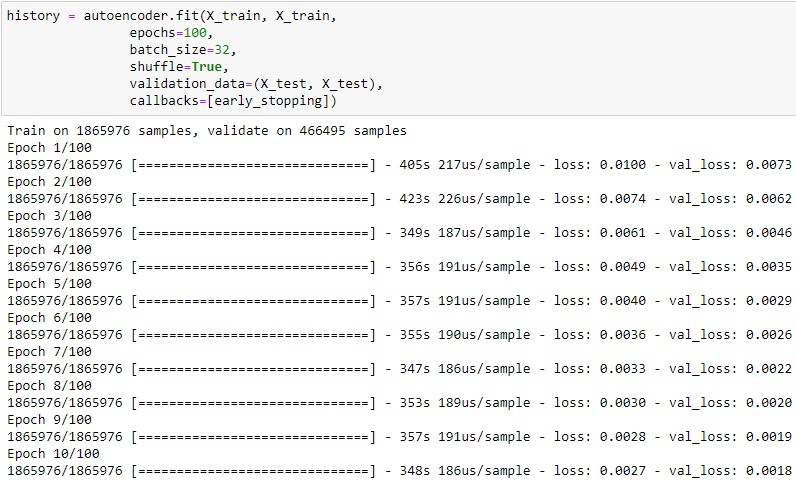
\includegraphics[width=\textwidth]{img/Entrenamiento autoencoder.jpg}        
    \end{minipage}

    \begin{minipage}[t]{0.9\textwidth}
        Fuente: Elaboración propia.
    \end{minipage}
\end{figure}

\subsection{Resultados y Evaluación}

El modelo final demostró una sólida capacidad de reconstrucción y no mostró signos de sobreajuste, como se evidencia en los gráficos de pérdida de entrenamiento. Este autoencoder está ahora listo para ser utilizado para transformar los datos en una representación de menor dimensión, lo cual facilitará la aplicación de técnicas de clustering para la segmentación de usuarios y la detección de patrones de comportamiento anómalos.

\begin{figure}[H]
    \begin{minipage}[t]{0.9\textwidth}
        \caption{Gráfico del entrenamiento del modelo autoencoder}
        \label{gráfico_autoencoder}        
    \end{minipage}

    \vspace{10pt}

    \begin{minipage}[b]{0.9\textwidth}
        \centering
        \includegraphics[width=\textwidth]{img/Gráfico entrenamiento autoencoder.png}        
    \end{minipage}

    \begin{minipage}[t]{0.9\textwidth}
        Fuente: Elaboración propia.
    \end{minipage}
\end{figure}

\subsection{Conclusión del Modelo de Autoencoder}

El autoencoder se diseñó para transformar datos de alta dimensión en una representación de menor dimensionalidad, lo cual es un paso fundamental en el pre-procesamiento para algoritmos de clustering.

Sin embargo, el propósito inicial del autoencoder no era predecir comportamientos futuros o tendencias, sino más bien identificar patrones intrínsecos y datos atípicos dentro del conjunto de datos existente. Dado que el objetivo central del proyecto es la predicción del comportamiento, se ha determinado que el autoencoder no cumple con los requisitos necesarios para avanzar hacia este nuevo objetivo.

Por tanto, hemos decidido no continuar con el desarrollo e implementación de este modelo en su forma actual. En cambio, nos enfocaremos en la búsqueda y aplicación de modelos predictivos más adecuados que estén alineados con las metas de pronosticar el comportamiento futuro y que puedan ofrecer insights más directos para la toma de decisiones y estrategias proactivas.

Este cambio de dirección subraya la importancia de una alineación clara entre las herramientas de modelado seleccionadas y los objetivos específicos del proyecto. Aunque el autoencoder es una herramienta poderosa para ciertas aplicaciones, en este caso, se ha reconocido que no es la solución óptima para las necesidades proyectadas.

Sin embargo, es importante destacar que el autoencoder es una herramienta extremadamente útil para identificar anomalías en patrones de comportamiento.


\section{Modelo de predicción secuencial}
Se implementó un modelo de clasificación con el propósito de predecir y comprender el comportamiento del usuario basándose en un conjunto de datos detallado y complejo.

\subsection{Preprocesamiento y Preparación de Datos}

Comenzamos con la importación de los datos desde un archivo CSV, seguida de un proceso de limpieza para asegurar la integridad de la información. En esta etapa, se filtraron registros específicos en la columna “método” y se descartaron aquellos casos donde la columna “canal” estaba vacía. Adicionalmente, las marcas temporales fueron convertidas al formato UTC para garantizar una estandarización completa a lo largo del conjunto de datos.

\subsection{Ordenamiento y Etiquetado}

Ordenamos el conjunto de datos cronológicamente por usuario y fecha de evento, para preservar la secuencia de acciones de cada usuario. Se generaron nuevas columnas que indican el siguiente método y canal utilizado por el usuario, sirviendo estas como etiquetas para el modelo de predicción que estamos diseñando.

\subsection{Identificación de Sesiones}

Calculamos el intervalo de tiempo entre eventos consecutivos para determinar el inicio de nuevas sesiones de usuario, basándonos en un umbral de tiempo preestablecido. Este umbral se seleccionó de acuerdo con la dinámica típica observada en el sitio web, considerando que una sesión representa un conjunto continuo de interacciones del usuario.

\subsection{Codificación de Categorías}

Dado que los métodos y canales son variables categóricas, los convertimos en representaciones numéricas utilizando diccionarios que asignan un valor entero único a cada categoría. Este paso es esencial para que los datos puedan ser interpretados y procesados por la red neuronal.

\subsection{Construcción de Secuencias}

Integramos las representaciones numéricas de los métodos y canales en secuencias de pares, correspondientes a cada sesión de usuario. Este enfoque nos permite modelar la secuencia de interacciones y la trayectoria de comportamiento de los usuarios.

\subsection{División de Datos}

Los datos fueron divididos en conjuntos de entrenamiento y prueba, lo que nos permite validar la capacidad del modelo de generalizar y realizar predicciones precisas en datos que no ha visto previamente.

\subsection{Construcción del Modelo}

Desarrollamos un modelo secuencial con la biblioteca Keras que incorpora capas de incrustación (Embedding) y LSTM. La capa de Embedding transforma nuestras representaciones numéricas en vectores de características densas, mientras que las capas LSTM se encargan de capturar las dependencias temporales y secuenciales presentes en los datos.


\begin{figure}[H]
    \begin{minipage}[t]{0.9\textwidth}
        \caption{Construccion del modelo de clasificación}
        \label{parquitectura_clasificación}        
    \end{minipage}

    \vspace{10pt}

    \begin{minipage}[b]{1\textwidth}
        \centering
        \includegraphics[width=\textwidth]{img/Arquitectura modelo clasificación.jpg}        
    \end{minipage}

    \begin{minipage}[t]{0.9\textwidth}
        Fuente: Elaboración propia.
    \end{minipage}
\end{figure}

\subsection{Regularización y Compilación}

Para combatir el sobreajuste, incluimos capas de Dropout después de cada capa LSTM, lo cual ayuda a que el modelo sea más robusto y menos propenso a memorizar los datos de entrenamiento. Posteriormente, compilamos el modelo con la función de pérdida de entropía cruzada categórica y el optimizador Adam para iniciar el proceso de aprendizaje.

\subsection{Entrenamiento del Modelo}

El modelo se entrenó utilizando tanto la precisión como la pérdida de validación como métricas clave para monitorear su rendimiento. Empleamos un callback de EarlyStopping que detiene el entrenamiento si no se observan mejoras en la pérdida de validación tras un cierto número de épocas. Además, este callback está configurado para restaurar los pesos del modelo al estado en que se obtuvo el mejor rendimiento en el conjunto de validación.

\subsection{Resultados del entrenamiento del modelo}

Después de completar el entrenamiento del modelo, evaluamos su rendimiento analizando las métricas de pérdida y precisión tanto en el conjunto de entrenamiento como en el de validación.

\begin{itemize}
    \item \textbf{Análisis de la Pérdida:} Los gráficos muestran que la pérdida de entrenamiento (Loss) y la pérdida de validación (Val\_Loss) disminuyen significativamente en las primeras épocas, lo que indica que el modelo está aprendiendo efectivamente de los datos. A medida que avanzan las épocas, ambas curvas de pérdida se estabilizan y convergen, lo que sugiere que el modelo ha alcanzado un punto donde realiza predicciones consistentes y fiables. La convergencia cercana de las dos líneas sugiere que el modelo no está sobreajustando, ya que la pérdida de validación no está aumentando ni divergiendo de la pérdida de entrenamiento.
    \item \textbf{Análisis de la Precisión:} En cuanto a la precisión, observamos que tanto la precisión de entrenamiento (Accuracy) como la precisión de validación (Val\_Accuracy) aumentan rápidamente y luego se estabilizan, manteniéndose muy cerca una de la otra. Esto indica un alto nivel de precisión en las predicciones del modelo y sugiere que el modelo generaliza bien a nuevos datos.
\end{itemize}

\begin{figure}[H]
    \begin{minipage}[t]{0.9\textwidth}
        \caption{Gráficos de análisis del modelo de clasificación}
        \label{gráfico_clasificación}        
    \end{minipage}

    \vspace{10pt}

    \begin{minipage}[b]{1\textwidth}
        \centering
        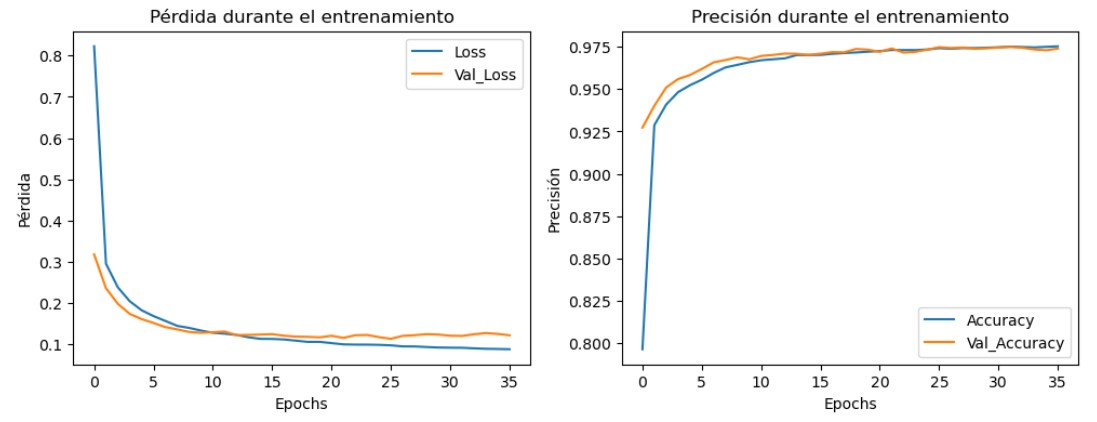
\includegraphics[width=\textwidth]{img/Gráfico modelo clasificación.jpg}        
    \end{minipage}

    \begin{minipage}[t]{0.9\textwidth}
        Fuente: Elaboración propia.
    \end{minipage}
\end{figure}

\subsection{Predicción del modelo}

Al realizar predicciones con el modelo, se utiliza una secuencia de acciones previas del usuario para predecir su siguiente acción. El modelo no solo proporciona la acción más probable sino también la confianza en su predicción, medida como una probabilidad.

Por ejemplo, si el modelo predice que el usuario seleccionará el método 'getDetails()' a continuación, también proporcionará la probabilidad asociada con esa predicción, por ejemplo, un 95\%. 

Otro ejemplo es con el método 'getAccounts()' el cual predice lo siguiente: El siguiente método predicho es: getSSContributionsCertificate() con una probabilidad del 78.76\%

\section{Tabla resumen métricas de los métodos aplicados}
\renewcommand{\tablename}{Tabla}


A continuación, se presenta una tabla que resume las distintas métricas ocupadas para conocer la precisión de los modelos aplicados.

Al tener 3 tipos de modelos distinos, las métricas varian entre cada uno de ellos, para el modelo arima las métricas representan el error que el modelo tiene al predecir una serie de tiempo, mientras más cercano a 0, mayor es su precisión y para el modelo secuencial las métricas representan la precisión de la predicción del modelo de clasificación.

\begin{center}
        \begin{tabular}{|c|c|c|c|c|c|c|}
            \multicolumn{7}{c}%
            {{\tablename\ Métricas.1 -- Tabla resumen métricas de métodos aplicados}} \\
            \hline
            \multirow{2}{*}{\textbf{Modelos aplicados}} &
                \multicolumn{6}{c|}{\textbf{Métricas}} \\
            \cline{2-7}
            & Precission & Recall & F1 Score & MAE & MSE & RMSE\\
            \hline
            Modelo ARIMA & - & - & - & 17.87 & 372.87 & 19.31 \\
            \hline
            Modelo Secuencial & 57.94\% & 54.87\% & 53.66\% & - & -& - \\
            \hline
        \end{tabular}
\end{center}

A raíz de nuestra decisión de no continuar con el desarrollo del modelo de autoencoders, nos encontramos en la situación de no contar con métricas de desempeño para este modelo en nuestro proyecto. Esta decisión se basa en el reconocimiento de que el autoencoder, aunque eficaz en la identificación de patrones y anomalías dentro de datos de alta dimensión, no se alinea con nuestra necesidad de predecir comportamientos y tendencias futuras. Dado que las métricas de desempeño para autoencoders están diseñadas principalmente para evaluar la precisión en la reconstrucción de datos y no para medir la efectividad en la predicción de eventos futuros, estas métricas resultan irrelevantes para nuestros objetivos. Por ende, al descartar el uso del autoencoder, también descartamos la aplicación de sus métricas asociadas, orientándonos ahora hacia la búsqueda de otros modelos predictivos que posean métricas de desempeño alineadas con nuestra meta de anticipar y actuar sobre futuros comportamientos y tendencias.

\chapter{Api y modelo implementado}
\input{Api y modelo/Descripción componentes.tex}

\section{Desarrollo e Implementación de la API}
\input{Api y modelo/Implementación API.tex}

\section{Dockerización de la Api}
\input{Api y modelo/Dockerización API.tex}

\chapter{Conclusión y Recomendación}
\subsection{Conclusión}

El desarrollo de este proyecto de tesis ha abarcado una gama integral de procesos y análisis, comenzando con un estudio bibliométrico y extendiéndose a través del proceso ETL (Extracción, Transformación y Carga), el Análisis Exploratorio de Datos (EDA) y la implementación y evaluación de modelos predictivos.

El estudio bibliométrico proporcionó una base sólida y rigurosa, permitiendo una comprensión profunda del estado actual del campo, identificando las tendencias predominantes y las áreas menos exploradas en la literatura. Este análisis ayudó a orientar el enfoque del proyecto hacia áreas de investigación que son tanto innovadoras como de relevancia práctica.

En la fase de ETL, se trabajó meticulosamente para asegurar la calidad y la integridad de los datos. Este proceso fue crucial para preparar un conjunto de datos coherente y fiable, lo que sentó las bases para un análisis más detallado y preciso. La limpieza, transformación y enriquecimiento de los datos fueron pasos fundamentales que garantizaron la confiabilidad de las conclusiones y recomendaciones posteriores.

El Análisis Exploratorio de Datos (EDA) permitió una comprensión más profunda de los datos a mano. A través de este análisis, se identificaron patrones, anomalías y relaciones clave que influyeron significativamente en la selección y el ajuste de los modelos predictivos. Esta fase fue vital para la comprensión de las dinámicas subyacentes de los datos y para formular hipótesis informadas para la modelización.

Finalmente, la fase de modelado y pruebas fue el núcleo del proyecto. La aplicación de modelos predictivos, ajustados y evaluados cuidadosamente, proporcionó insights valiosos y respuestas a las preguntas de investigación planteadas. La evaluación de estos modelos, utilizando métricas como la precisión, el recall y la puntuación F1, reveló un rendimiento moderado, indicando áreas para futuras mejoras y ajustes. Esta fase no solo validó el enfoque metodológico empleado, sino que también abrió caminos para futuras investigaciones y desarrollos.

En conjunto, este proyecto ha demostrado la importancia de un enfoque metódico y bien estructurado en la investigación. Desde la recopilación inicial de datos hasta el análisis final y la interpretación de los resultados, cada etapa ha sido crucial para construir un entendimiento completo del tema en cuestión. Las lecciones aprendidas y los conocimientos adquiridos durante este proyecto no solo son valiosos para este campo de estudio, sino que también proporcionan un marco para futuras investigaciones y desarrollos en áreas relacionadas.


\subsection{Recomendaciones}

A través del desarrollo de este proyecto, se han identificado varias áreas clave en las que se pueden realizar mejoras y avances. Estas recomendaciones están orientadas a optimizar el modelo actual y a expandir el alcance de la investigación futura:

\subsubsection{Optimización del Modelo Actual:}
\begin{itemize}
    \item \textbf{Aumentar el Conjunto de Datos:} Un mayor volumen de datos puede mejorar la capacidad del modelo para aprender y generalizar. Esto es especialmente relevante en modelos basados en aprendizaje profundo que requieren grandes cantidades de datos para un rendimiento óptimo.
    \item \textbf{Exploración de Hiperparámetros:} Ajustar los hiperparámetros del modelo, como la tasa de aprendizaje, el número de capas ocultas y la cantidad de nodos en cada capa, puede resultar en mejoras significativas en el rendimiento.
    \item \textbf{Incorporación de Regularización:} Implementar técnicas de regularización como Dropout o L1/L2 puede ayudar a prevenir el sobreajuste y mejorar la generalización del modelo en datos no vistos.
\end{itemize}

\subsubsection{Experimentación con Diferentes Arquitecturas de Modelos:}
\begin{itemize}
    \item \textbf{Modelos de Aprendizaje Profundo Avanzados:} Probar con arquitecturas más complejas, como Redes Neuronales Recurrentes (RNN), Transformers o modelos basados en atención, podría capturar mejor las relaciones temporales y contextuales en los datos.
    \item \textbf{Enfoque Híbrido:} Combinar modelos de aprendizaje automático tradicionales con técnicas de aprendizaje profundo puede proporcionar una visión más holística y mejorar la precisión de las predicciones.
\end{itemize}

\subsubsection{Análisis de Características Adicionales:}
\begin{itemize}
    \item \textbf{Ingeniería de Características:} Explorar nuevas características derivadas de los datos existentes puede revelar patrones ocultos y mejorar la capacidad predictiva del modelo.
    \item \textbf{Integración de Datos Externos:} Incorporar datos externos, como tendencias de mercado o indicadores económicos, podría proporcionar contextos adicionales que mejoren la precisión predictiva.
\end{itemize}

\subsubsection{Evaluación Continuada y Ajuste del Modelo:}
\begin{itemize}
    \item \textbf{Monitoreo de Desempeño en Tiempo Real:} Establecer un sistema de monitoreo para evaluar el desempeño del modelo en tiempo real puede ayudar a identificar rápidamente áreas de mejora y ajustar el modelo de manera proactiva.
    \item \textbf{Actualización de Datos y Modelos:} Regularmente actualizar el modelo con nuevos datos para mantener su relevancia y precisión frente a patrones cambiantes y tendencias emergentes.
\end{itemize}

\subsubsection{Investigaciones Futuras:}
\begin{itemize}
    \item \textbf{Estudio de Casos Específicos:} Investigar en profundidad casos específicos donde el modelo no se desempeñó según lo esperado puede proporcionar insights valiosos para futuras mejoras.
    \item \textbf{Expansión a Nuevos Dominios:} Aplicar el modelo a diferentes conjuntos de datos o en distintos contextos podría ayudar a evaluar su robustez y adaptabilidad.
\end{itemize}

Estas recomendaciones están destinadas a guiar los esfuerzos futuros hacia la mejora continua del modelo y la expansión del conocimiento en este campo de estudio. La implementación exitosa de estas sugerencias requiere un enfoque iterativo y adaptable, asegurando que el modelo se mantenga relevante y efectivo frente a las cambiantes dinámicas de datos y requerimientos del mundo real.

\begin{doublespace}
  \bibliographystyle{apacite}
  \bibliography{Bibliografia}
\end{doublespace}

\chapter*{Anexos}
\addcontentsline{toc}{chapter}{Anexos}
\section*{Anexo 1. Listado de métodos en la plataforma}
\addcontentsline{toc}{section}{Anexo 1. Listado de métodos en la plataforma}
\begin{tabular}{|p{6cm}|p{8cm}|}
    \hline
    \multicolumn{1}{|c|}{\textbf{Método}} & \multicolumn{1}{c|}{\textbf{Descripción}} \\
    \hline
    login() & Login a app o web \\
    getMensualpdf() &	Obtiene cartola mensual \\
    getAccountWithdrawal() &	Obtiene Cuentas para realizar giros APV y CAV \\
    getAccounts() &	Obtiene Cuentas del Cliente \\
    getProfitabilityVSContributions() &	Información de Aportes Versus Rentabilidad \\
    getProfitabilityAccountByPeriod() &	Información de Rentabilitad por Periodo asociada a CArtola Mensual \\
    getApplications() &	Lista solicitudes de cambio y distribución de fondos \\
    getSocialSecurityContribution() &	Obtiene Cotizaciones por producto de los clientes \\
    getAccountsConditions() &	Obtiene precondiciones para realizar Cambio/Distribución de Fondos \\
    getRecognitionBonds() &	Obtiene bono de reconocimiento \\
    getShareValues() &	Obtiene valores cuota \\
    obtenerSaldos() &	Obtiene saldos del cliente \\
    obtenerBeneficiarios() &	Obtiene beneficiarios registrados por el cliente \\
    datosPersonales() &	Obtiene datos personales del cliente \\
    getBankAccount() &	Obtiene lista de bancos \\
    getDatosPersonales() &	Obtiene información personal del cliente \\
    getDatosRegiones() &	Obtiene listadod e regiones \\
    getDatosPaises() &	Obtiene listado de paises \\
    getDatosComunas() &	Obtiene el listado de comunas \\
    validateSecurityKey() &	Valida la clave de seguridad de previred \\
    getCuentas() &	Obtiene lista de cuentas del cliente \\
    conditionSecurityKey() &	Obtiene el estado de actual de la clave de seguridad \\
    getMensual() &	Obtiene información de la cartola mensual \\
    getCertificadoCotizaciones() &	Genera el PDF del certificado de cotización según el rango de fechas \\
    getPeriodosCuatrimestral() & Lista de periodos de consulta de la cartola cuatrimestral \\
    getProfitability() & Consulta colección de firebase de configuraciones el documento del listado de validaciones de seguridad \\
    getEnviarCuatrimestral() & Obtiene la cartola cuatrimestral \\
    getCertificadoAfiliacion() & Obtiene certificado de afiliación \\
    getCertificadoRemuneraciones() & Obtiene certificado de remuneraciones \\
    omnichannelLogin() & Autentifica Capa Omnicanal AFP \\
    RestructureFundsBusiness.restructureFunds() & Obtiene Comprobante en PDF de Cambio/Distribucion de Fondos \\
    restructureFunds() & Graba Cambio/Distribución de Fondos \\
    getCertificadoResidencia() & Obtiene certificado de residencia \\
    saveSurvey() & Guarda encuesta \\
    validateTemporalPassword() & Valida Clave Dinámica \\
    generateTemporalPassword() & Solicita Clave Dinámica \\
    getCertificadoAntecedentes() & Obtener Certificado Antecedentes Previsionales \\
    getCertificadoVacaciones() & Obtener Certificado Vacaciones Progresivas \\
    getCertificadoTrabajosPesados() & Obtener Certificado Trabajos Pesados \\
    generarContacto() & Enviar Formulario de Contacto a Ejecutivos \\
    editarDatosPersonales() & Actualizar Datos Personales \\
    sendSms() & Enviar SMS \\
    getCertificadoComprobante() & Obtener Certificado Comprobante de Pago Pensión \\
    getCertificadoPensionadosPagados() & Obtener Certificado de Pensiones Pagadas \\
    withdrawalRequest() & Grabar Giro APV/CAV Cliente \\
    getBankAccounts() & Obtener Cuentas Bancarias \\
    validarDatosContacto() & Validar DAtos de Contacto(Si están duplicados) \\
    validarListaNegra() & Validar Listado de Cuentas Email/Celular no Validas(Email y Celular) \\
    addBankAccount() & Agregar cuenta Bancaria de Cliente \\
    obtenerEstadoCuentaCorriente() & Obtener Estado de Cuenta Corriente(Banco Santander) \\
    validarCuentasDigitales() & Validar Cuentas Digitales \\
    getTypesBanksAccounts() & Obtener Tipos de Cuentas Bancarias \\
    sendEmail() & Enviar Email \\
    getCertificadoNoCotizados() & Obtener Certificado de Periodos No Cotizados \\
    deleteBankAccount() & Eliminar Cuenta Bancaria de Cliente \\
    addBeneficiarios() & Agrega beneficiarios de pensión del cliente \\
    changePassword() & Cambia la clave de seguridad \\
    getAttentionVideo() & Obtiene el agendamiento de video atención \\ 
    getCertificadoIngresoBase() & Obtiene el certificado de Ingreso Base para pensionados \\
    getChangesAndDistributionsOfFunds() &	Obtiene los cambios y distribuciones de fondos realizados \\
    getDetailRequestStateChangeFunds() &	Detalle estado de solicitudes de Cambio y Distribución de fondos \\
    getPensionBackgroundCert() &	Certificado de antecedentes previsionales para la APP \\
    getPensionsCertificate() &	Obtiene el certificado de pensiones \\
    getRemunerationsCert() &	Obtiene el certificado de remuneraciones imponibles \\
    getSSContributionsCertificate() &	Obtiene el certificado de cotizaciones \\
    getSimulationWithdrawalCAV() &	Realizar la simulación del giro de Cuenta 2 \\
    getWithdrawsAPV() &	Resumen de estado de solicitudes APV \\
    obtenerCodigoParentesco() &	Obtiene los códigos de parentesco para el ingreso de beneficiarios \\
    obtenerFichaCalculo() &	Obtiene el certificado de ficha de cálculo \\
    obtenerSaldos() &	Obtiene los saldos del cliente \\
    requestAfpPassword() &	Solicitud cambio de password \\
    sendComplaintForm() &	Envío de reclamo \\
    basicLogin() &	Datos básicos del cliente \\
    crearClave() &	Crea la clave de acceso \\
    getBeneficiarios() &	Obtiene los beneficiarios ingresados por el cliente \\
    getCertificadoTributario() &	Obtiene los certificados tributarios \\
    getContactCategories() &	Obtiene las categorías del formulario de contacto \\
    getMembershipCert() &	Obtiene el certificado de afiliación \\
    getPensionTramite() &	Obtiene el certificado de pensión en trámite \\
    getPersonStatus() &	Indica si es cliente nuevo y/o activo, si tiene password de 4 o 6 digitos \\
    getRetireeQualityCertificate() &	Certificado de calidad de pensionado en la APP \\
    getSimulationWithdrawalAPV() &	Realizar la simulación del giro de APV \\
    getVacationsCert() &	Obtiene el certificado de vacaciones progresivas \\
    getWithdrawsCAV() &	Resumen de estado de solicitudes Cuenta dos \\
    obtenerEstadoClave() &	Obtiene el estado de la clave de seguridad \\
    obtenerListaParentescoFormulario() &	Obtiene la lista de parentescos del formulario de beneficiarios \\
    reCaptcha() &	Ejecuta el recaptcha de google \\
    sendComplaintFile() &	Adjunta documentos al formulario de reclamo desde el front \\
    sendContactCases() &	Solicitud de contacto \\
    cambiarClaveAcceso() &	Cambia la clave de 6 dígitos del cliente \\
    existeFichaCalculo() &	Busca si existe la ficha de cálculo \\
    getRegiones() &	Obtiene la lista de regiones \\
    loginApplication() &	Recupera token de sesion de apiconnect \\
    recuperarClave() &	Recupera la clave de seguridad \\
    sendEmailPubsub() &	Envío de email \\    
    \hline
\end{tabular}

\end{document}